\documentclass[12pt]{book}
\usepackage[pages=some]{background}
\usepackage[default]{lato}
\usepackage[spanish]{babel}
\usepackage[square,sort,comma,numbers]{natbib}
\usepackage{url}
\usepackage[utf8x]{inputenc}
\usepackage{amsmath}
\usepackage{graphicx}
\graphicspath{{images/}}
\usepackage{parskip}
\usepackage{fancyhdr}
\usepackage{vmargin}
\usepackage{xcolor}
\usepackage{sectsty}
\usepackage{titlesec}
\usepackage{hyperref}
\usepackage{enumerate}
\usepackage{etoolbox}

\definecolor{uca-blue}{HTML}{0e617f}
\definecolor{uca-orange}{HTML}{df872e}

%chapterfont{\color{blue}}  
\sectionfont{\color{uca-orange}}
\subsectionfont{\color{uca-blue}}

\titleformat{\subsubsection}
  {\color{uca-blue}\normalfont\fontfamily{lato}\fontsize{14}{17}\selectfont}{\thesubsubsection}{0.75em}{}
  
\makeatletter
\patchcmd{\f@nch@head}{\rlap}{\color{uca-orange}\rlap}{}{}
\patchcmd{\headrule}{\hrule}{\color{uca-orange}\hrule}{}{}
\makeatother
  

\backgroundsetup{
scale=1,
color=black,
opacity=0.9,
angle=0,
vshift=150mm,
contents={%
  
\includegraphics[width=2\paperwidth,height=0.75\paperheight]{images/portada.jpg}
  }%
}
\setmarginsrb{3 cm}{2.5 cm}{3 cm}{2.5 cm}{1 cm}{1.5 cm}{1 cm}{1.5 cm}


\pagestyle{fancy}
\fancyhf{}
\lhead{Seguridad en los Sistemas Informáticos}
\rhead{Grupo 9, Prácticas 3 y 4}


\cfoot{\thepage}

\begin{document}

%%%%%%%%%%%%%%%%%%%%%%%%%%%%%%%%%%%%%%%%%%%%%%%%%%%%%%%%%%%%%%%%%%%%%%%%%%%%%%%%%%%%%%%%% 

\begin{titlepage}
    \BgThispage

    \vspace*{\fill}
    %Se deberá introducir el número y título de la práctica. Si queda demasiado grande, puedes sustituir la etiqueta \Huge por \Large, o directamente eliminarla según tus necesidades.
    {\Huge\color{uca-blue}{Práctica 3: \textit{Recolección de información en fuentes abiertas I y II}} \par} %Sustituir por el número y nombre de la práctica
    {\Huge\color{uca-blue}{Práctica 4: \textit{Escaneo y enumeración de activos}} \par} %Sustituir por el número y nombre de la práctica
    {\Large\color{uca-blue}{Seguridad en los Sistemas Informáticos} \par}
    {\color{uca-blue}{Grupo 9} \par} %Sustituir por el número de grupo que realiza la práctica
    {\color{uca-orange}{Juan Antonio Pozo Orozco\\ %Introducir nombres completos.
                        José Manuel Gallardo del Águila\\
                        Jose Luis Venega Sánchez} 
                        \par}
    {\Large\color{uca-blue}{\textbf{CURSO 2024/25}} \par}
    %En el caso de haber menos integrantes, basta con eliminarlo de la lista.
    %Las dos líneas '\\' representan un salto de línea.
\end{titlepage}

%%%%%%%%%%%%%%%%%%%%%%%%%%%%%%%%%%%%%%%%%%%%%%%%%%%%%%%%%%%%%%%%%%%%%%%%%%%%%%%%%%%%%%%%%
%NO MODIFICAR: ESTO AUTOGENERARÁ EL ÍNDICE DEL DOCUMENTO
\tableofcontents
\pagebreak

%%%%%%%%%%%%%%%%%%%%%%%%%%%%%%%%%%%%%%%%%%%%%%%%%%%%%%%%%%%%%%%%%%%%%%%%%%%%%%%%%%%%%%%%%

\chapter{Práctica 3.1: Recolección de información en fuentes abiertas I}

\section{Ejercicio 1}
\textit{Accederemos al enlace cuya dirección es:\\ \url{http://www.cs.fsu.edu/~langley/CIS4385-2015-1/2015-01-logs-test/auth.log}.}

\textit{Conteste a las siguientes preguntas:}

\begin{itemize}
    \item \textit{¿A qué tipo de archivo estamos accediendo, y para qué sirve en los sistemas?}
    \newline
    Estamos accediendo a un fichero '.log' de una base de datos MySQL.
    \begin{figure}[h]
        \centering
        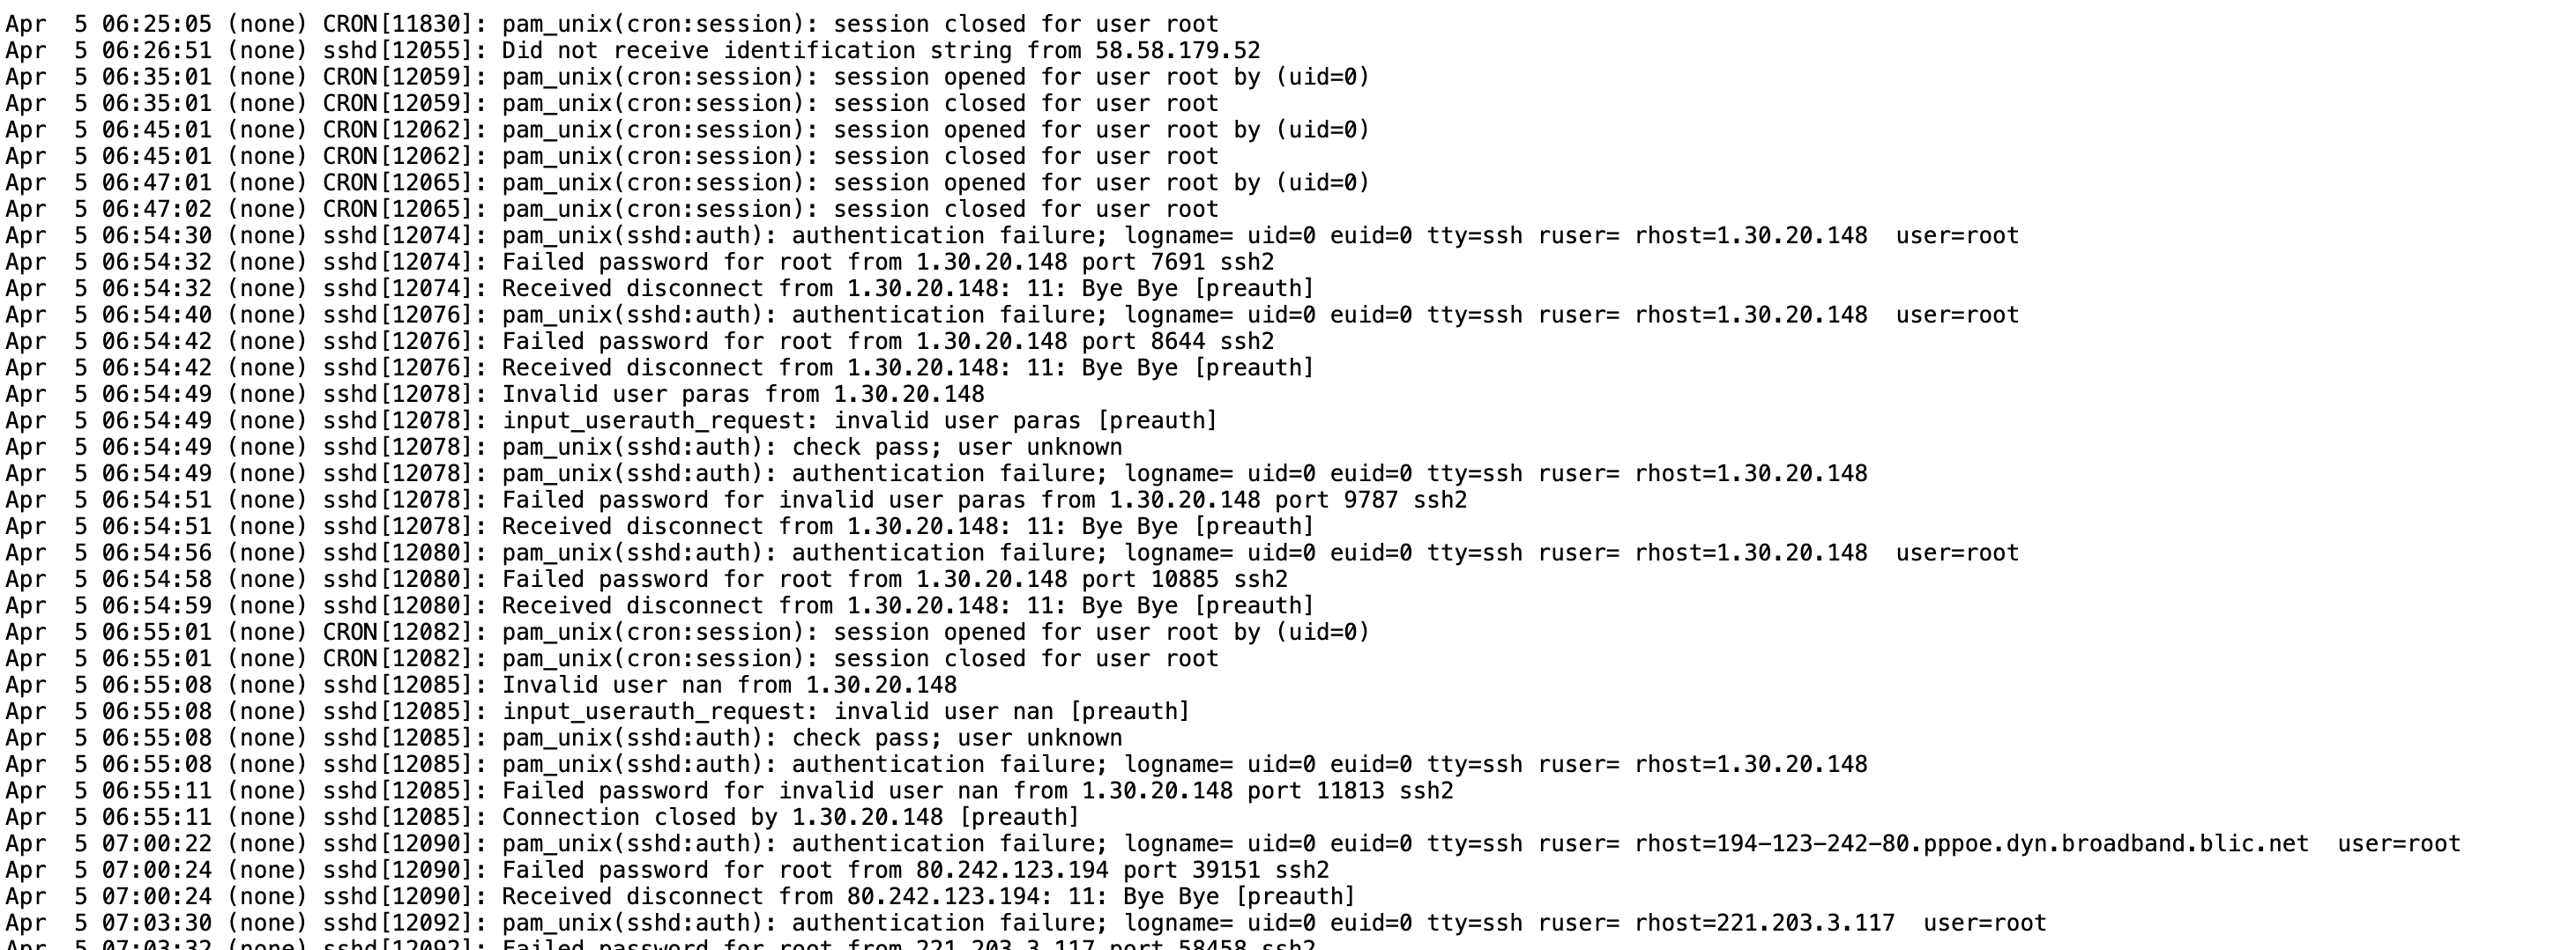
\includegraphics[width=\linewidth]{Practica 3y4/images/Screenshot 2024-10-24 at 09.15.20.png}
        \caption{Fragmento del contenido del archivo.log}
        \label{fig:enter-label}
    \end{figure}
    \item \textit{¿Qué información útil podríamos obtener de este archivo si nuestra finalidad fuera maliciosa?}
    \newline
    Podríamos obtener credenciales de usuarios o direcciones IPs que podamos encontrar en el propio fichero.
\end{itemize}

\textit{Ahora, accederemos al enlace \url{http://ftp.rinotel.com/Software/Linux/proftpd.conf}.}

\textit{Conteste a las siguientes preguntas:}

\begin{itemize}
    \item \textit{¿A qué tipo de archivo estamos accediendo, y para qué sirve en los sistemas?}
    \newline
    Estamos accediendo a un fichero de configuración ".conf", ya que en el dork estamos haciendo uso del parámetro \textbf{filetype .conf}.

    \begin{figure}[h]
        \centering
        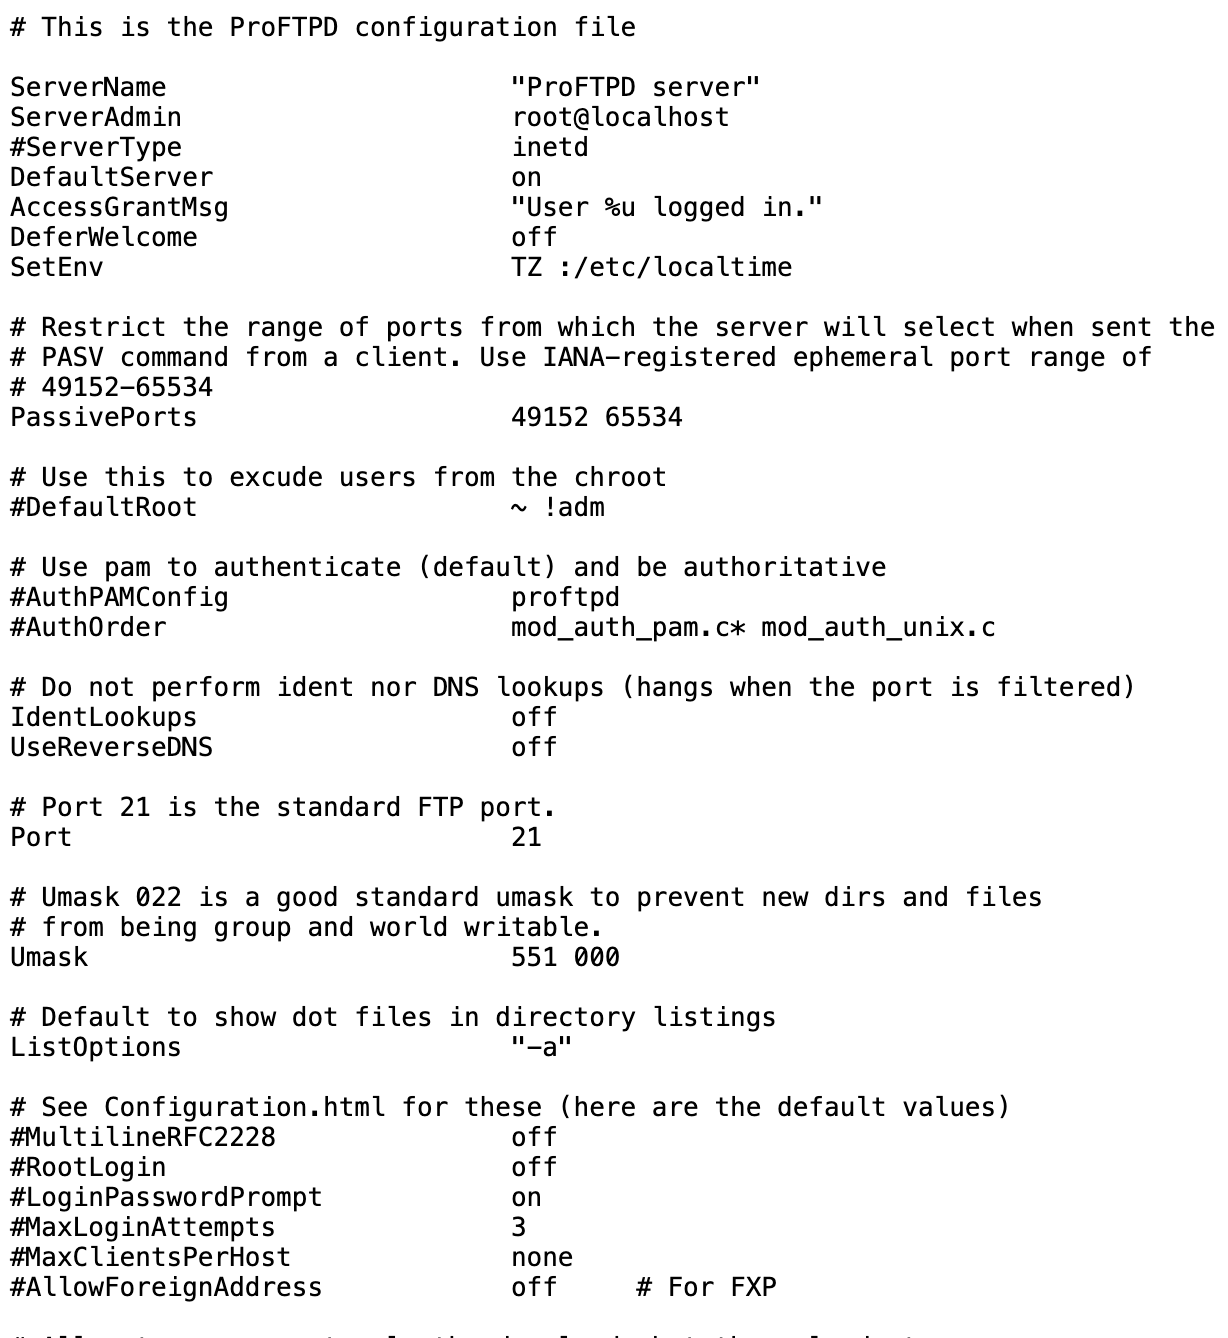
\includegraphics[width=.75\linewidth]{Practica 3y4/images/Screenshot 2024-10-24 at 09.37.30.png}
        \caption{Contenido del fichero.conf}
        \label{fig:enter-label}
    \end{figure}
    
    \item \textit{¿Qué información útil podríamos obtener de este archivo si nuestra finalidad fuera maliciosa?}
    \newline
    Tenemos un archivo de configuración '.conf' de un servicio \textit{PROFTPD}, el cual corre bajo el protocolo \textit{FTP}, por lo que podemos encontrar información sobre si la TLS está activada o no, o si podemos iniciar sesion con una conexión anónima.
\end{itemize}

\textit{Por último, accedemos al dork con título: filetype
username putty. Haremos clic en el enlace que aparece, cuya URL es \url{http://asanovich.free.fr/COMPASS/4-1.log}.}

\textit{Conteste a las siguientes preguntas:}

\begin{itemize}
    \item \textit{¿A qué tipo de archivo estamos accediendo, y para qué sirve en los sistemas?}
    \newline
    Estamos accediendo a un fichero de configuración de un dispositivo de red, el cual probablemente sea un switch.

\begin{figure}[h]
    \centering
    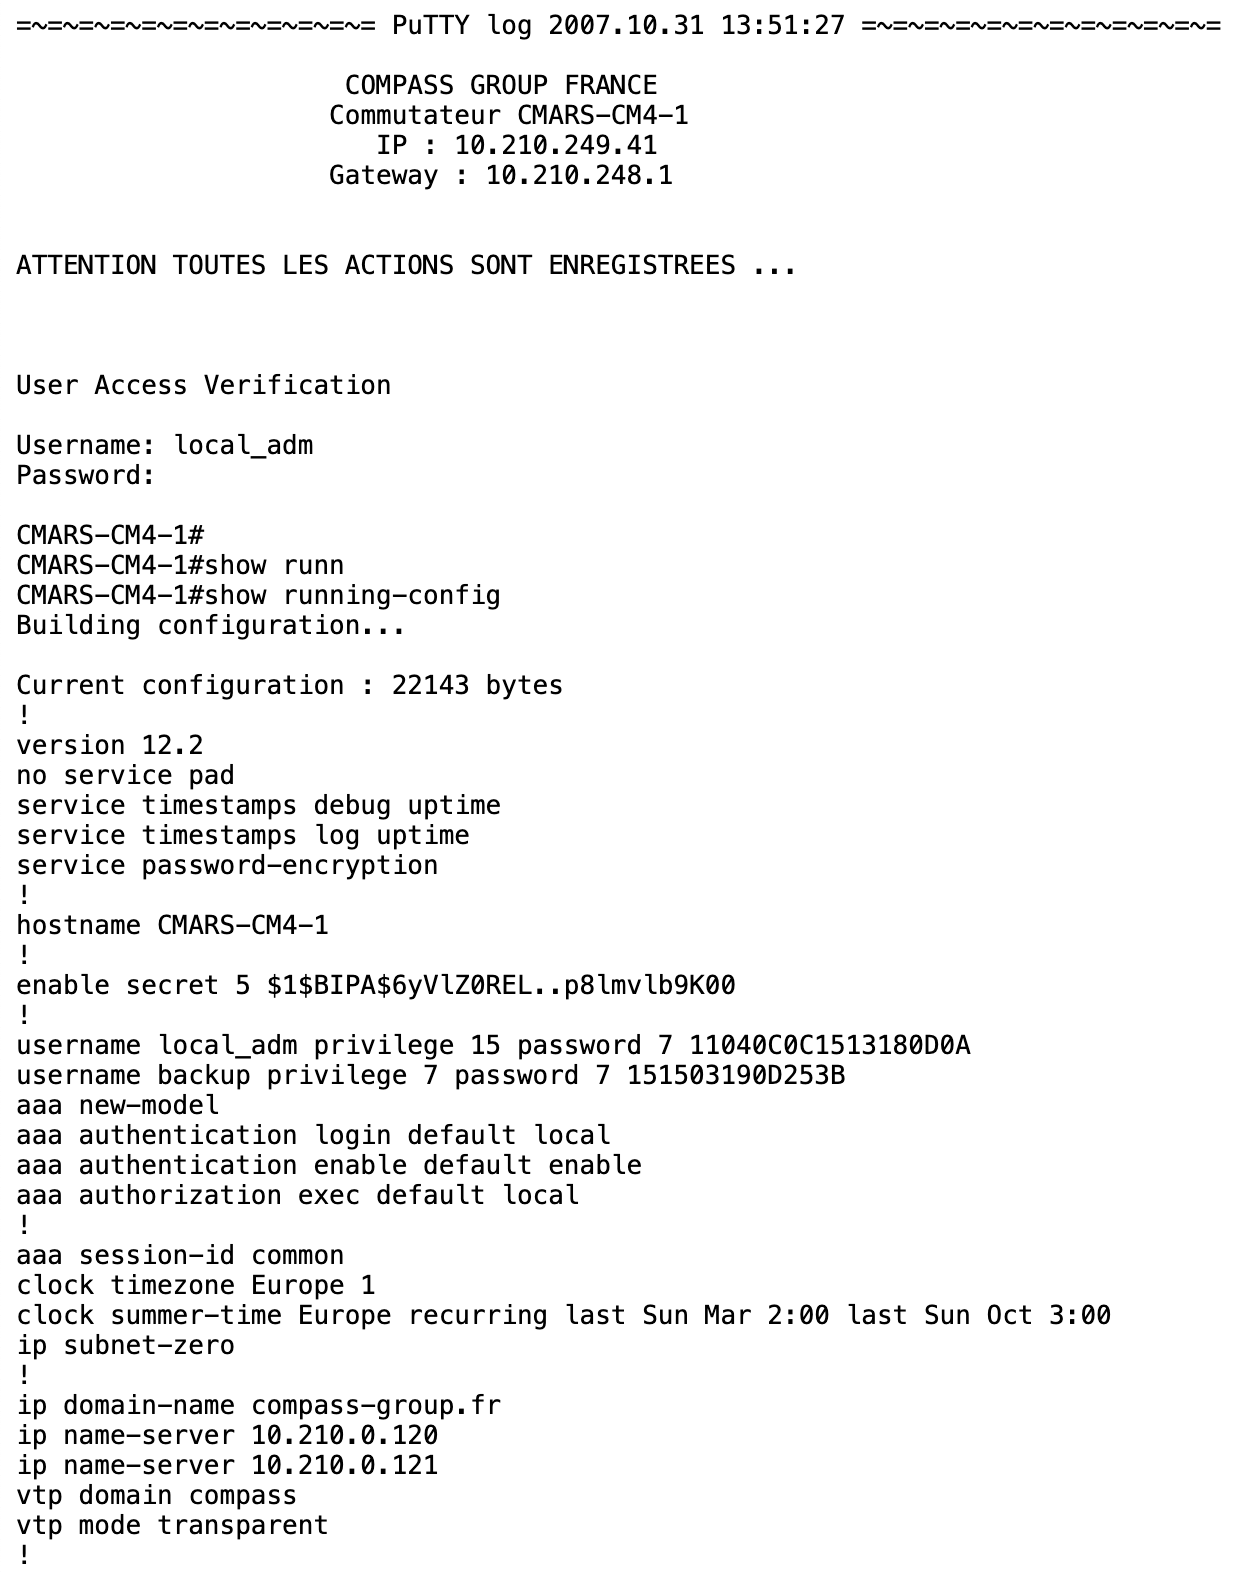
\includegraphics[width=0.5\linewidth]{Practica 3y4/images/Screenshot 2024-10-24 at 09.47.24.png}
    \caption{Parte del contenido de la configuración de un switch}
    \label{fig:enter-label}
\end{figure}
    \item \textit{¿Qué información útil podríamos obtener de este archivo si nuestra finalidad fuera maliciosa?}
    \newline
    Podemos encontrar version del software del propio switch, configuraciones y autenticación de usuarios, entre otros.
\end{itemize}

%%%%%%%%%%%%%%%%%%%%%%%%%%%%%%%%%%%%%%%%%%%%%%%%%%%%%%%%%%%%%%%%%%%%%%%%%%%%%%%%%%%%%%%%%

\section{Ejercicio 2}

\textit{Accedemos a la siguente URL \url{https://open-bitbucket.nrao.edu/projects/CASA/repos/casa-pkg/browse/configuration/jenkins/warp/users/ville/config.xml?at=67d6e09964459b6f0d7004b36efbaedcee575b3f}}

\begin{itemize}
    \item \textit{¿Qué tipo de archivo nos devuelve el uso de este dork?}
    \newline
    Nos devuelve archivos de tipo XML (observable en filetype:xml)
    \begin{figure}[h]
        \centering
        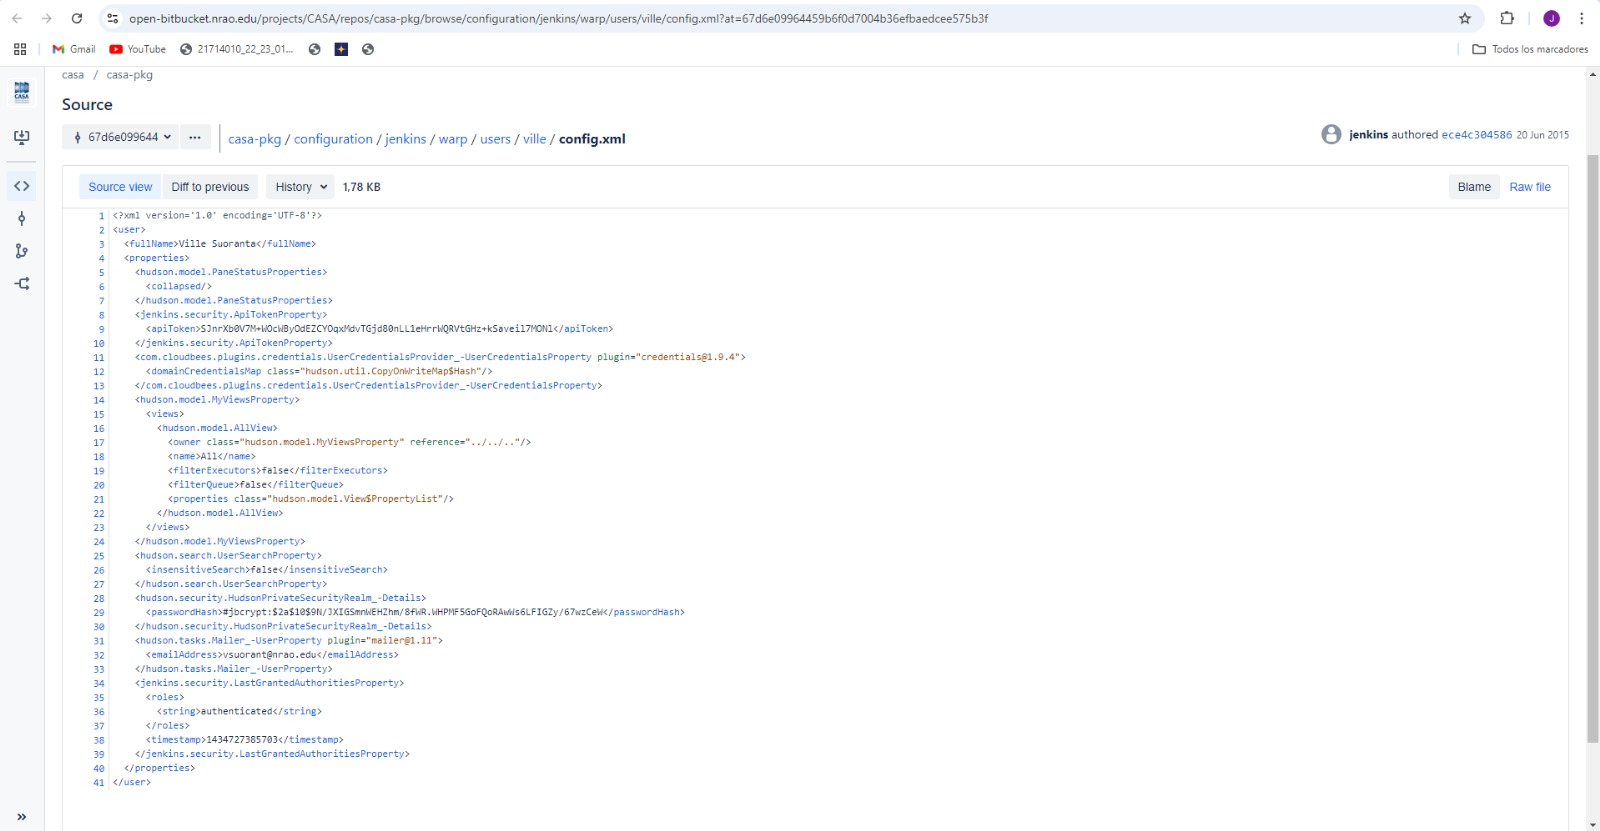
\includegraphics[width=\linewidth]{Practica 3y4/images/WhatsApp Image 2024-10-24 at 09.37.38.jpeg}
        \caption{Contenido del archivo XML.}
        \label{fig:enter-label}
    \end{figure}
    
    \item \textit{¿Qué información útil podríamos obtener de este archivo si nuestra finalidad fuera maliciosa}
    \newline
    Si un atacante accediera a este archivo tendría todo la información relacionada con el email y contraseña (mediante su hash) del usuario Ville Suoranta (líneas 29 y 32).
   
\end{itemize}

\textit{Ahora, accedemos a\\ \url{https://github.com/aptorres27/AnnalizaTorresPersonalWebsite/blob/master/proftpdpasswd}}
\begin{itemize}
    \item \textit{¿Qué información contienen estos archivos y para qué podría sernos útil dicha información si tuviéramos una intención maliciosa?}
    \newline
    Estos archivos pueden contener información sensible, como nombres de usuarios y contraseñas (hasheadas) como podemos ver en la \textit{Figura 1.4}.
\end{itemize}

%%%%%%%%%%%%%%%%%%%%%%%%%%%%%%%%%%%%%%%%%%%%%%%%%%%%%%%%%%%%%%%%%%%%%%%%%%%%%%%%%%%%%%%%%
\section{Ejercicio 3}
\textit{Seleccionamos la categoría “Web Server Detection” en Google Hacking Database, y buscamos el dork cuyo título es intext:"Powered by phpSQLiteCMS" | intitle:"phpSQLiteCMS - A simple \& lightweight CMS".
Al hacer esto llegaremos a un resultado de Google y accedemos a varios enlaces
devueltos por la búsqueda para detectar qu´e tipo de información nos devuelve la
búsqueda realizada.
Conteste a las siguientes preguntas:}
\begin{figure}[h]
    \centering
    \begin{minipage}{0.45\textwidth}
        \centering
        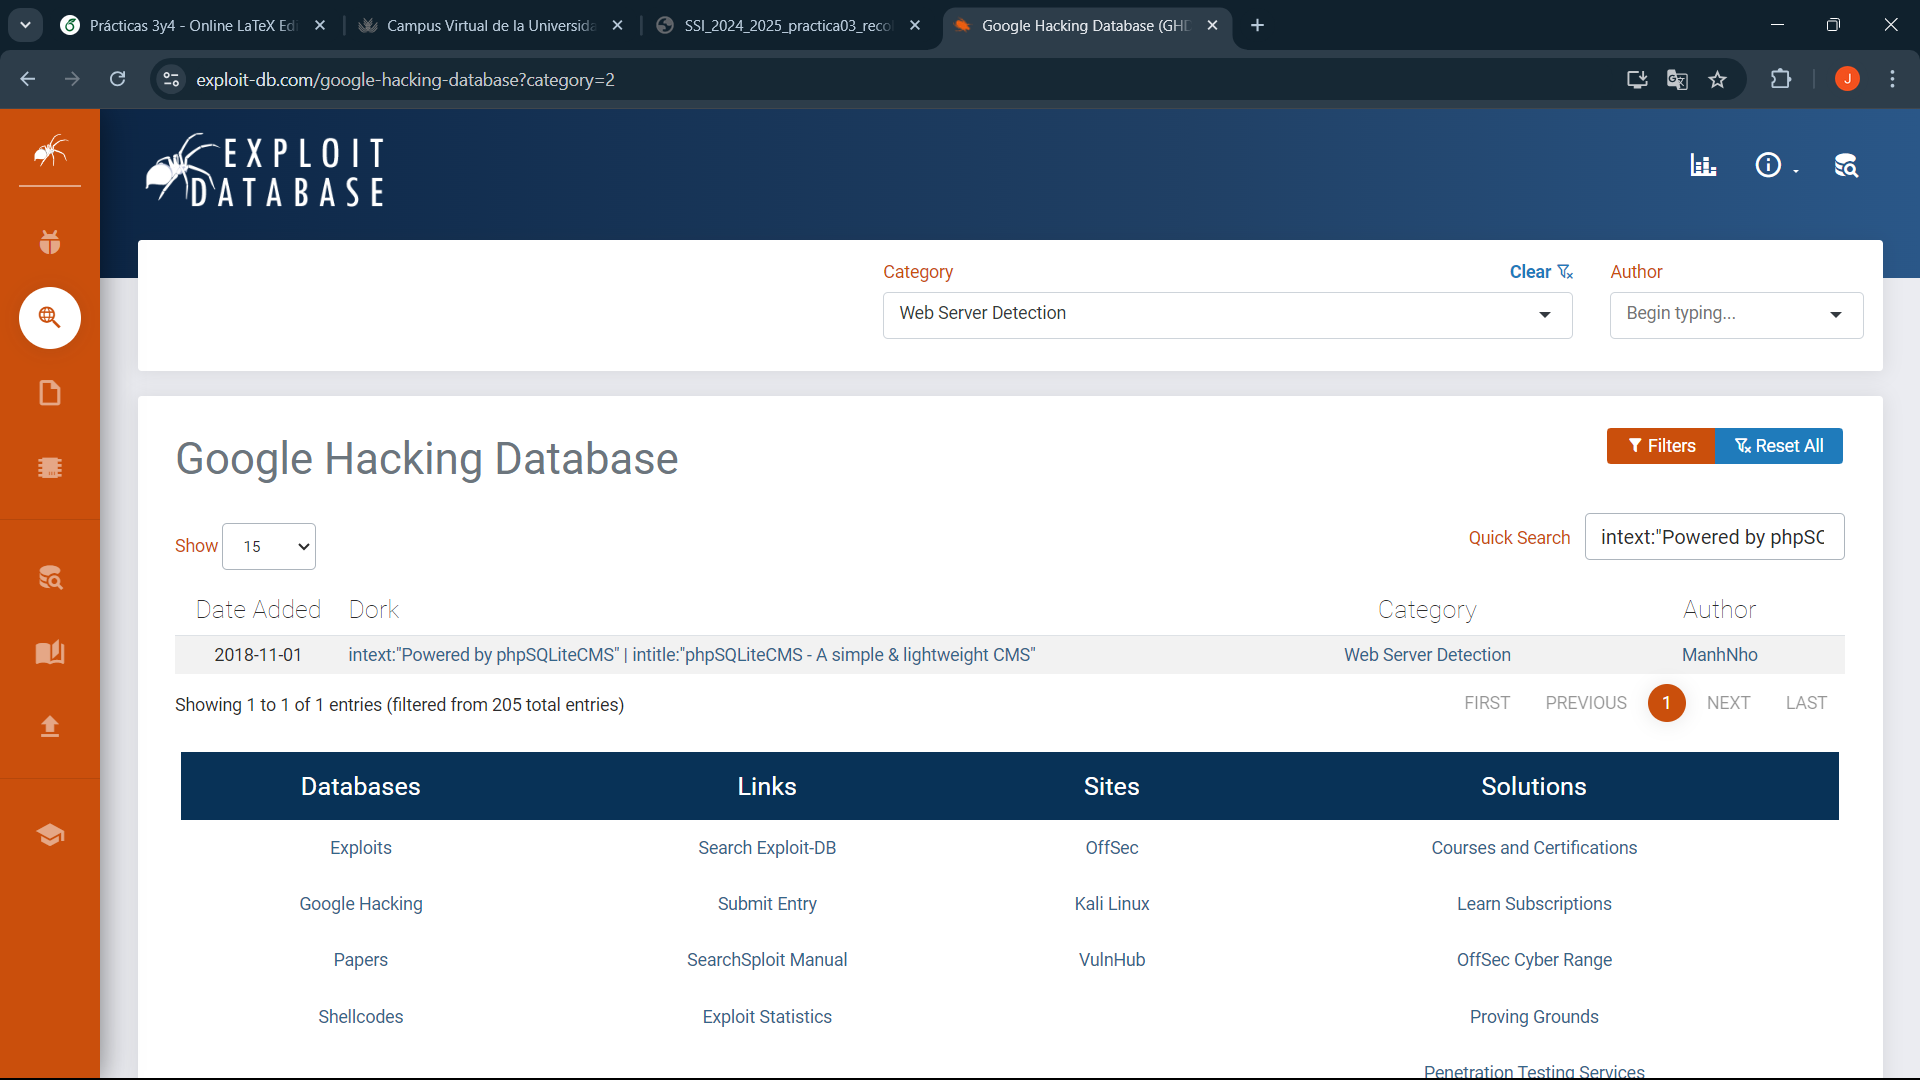
\includegraphics[width=\textwidth]{Practica 3y4/images/Captura de pantalla (80).png}
    \end{minipage}\hfill
    \begin{minipage}{0.45\textwidth}
        \centering
        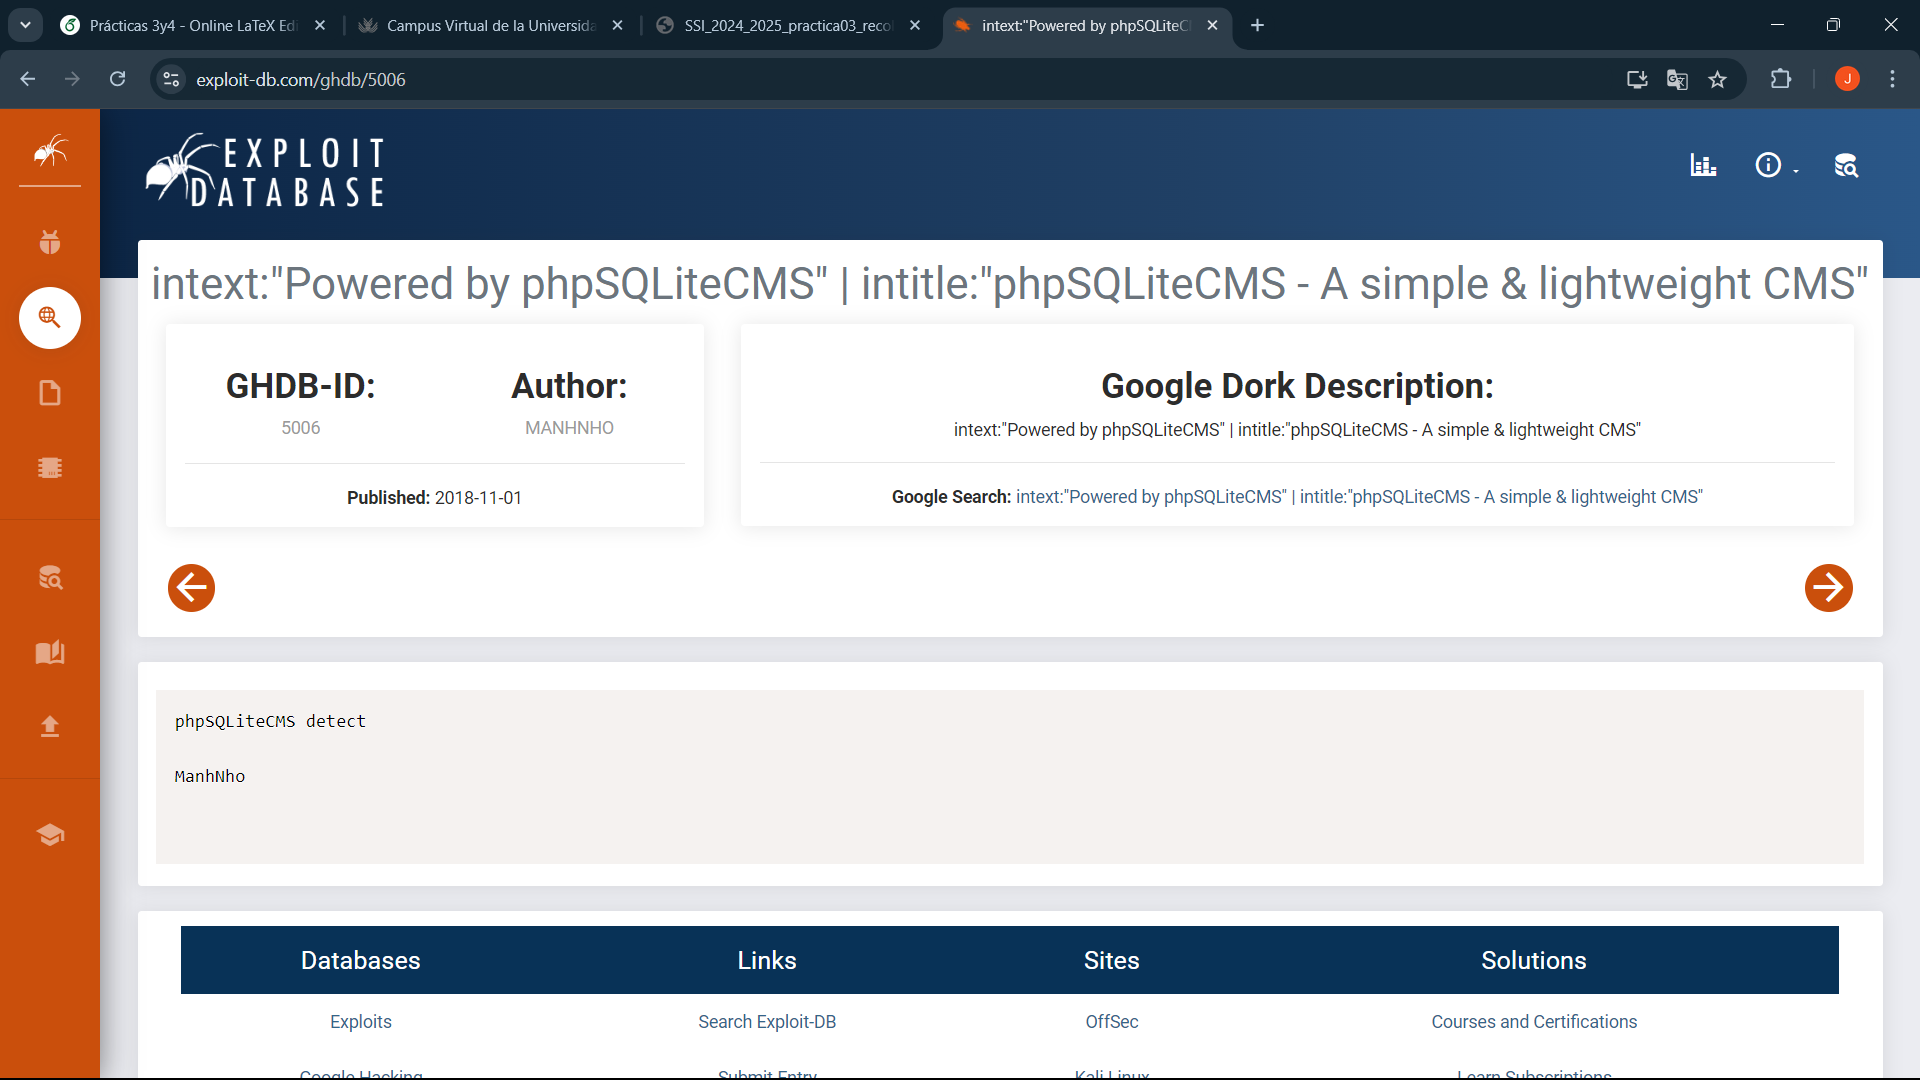
\includegraphics[width=\textwidth]{Practica 3y4/images/Captura de pantalla (81).png}
    \end{minipage}
    \caption{Búsqueda en Google Hacking Database}
\end{figure}
\begin{figure}[h]
    \centering
    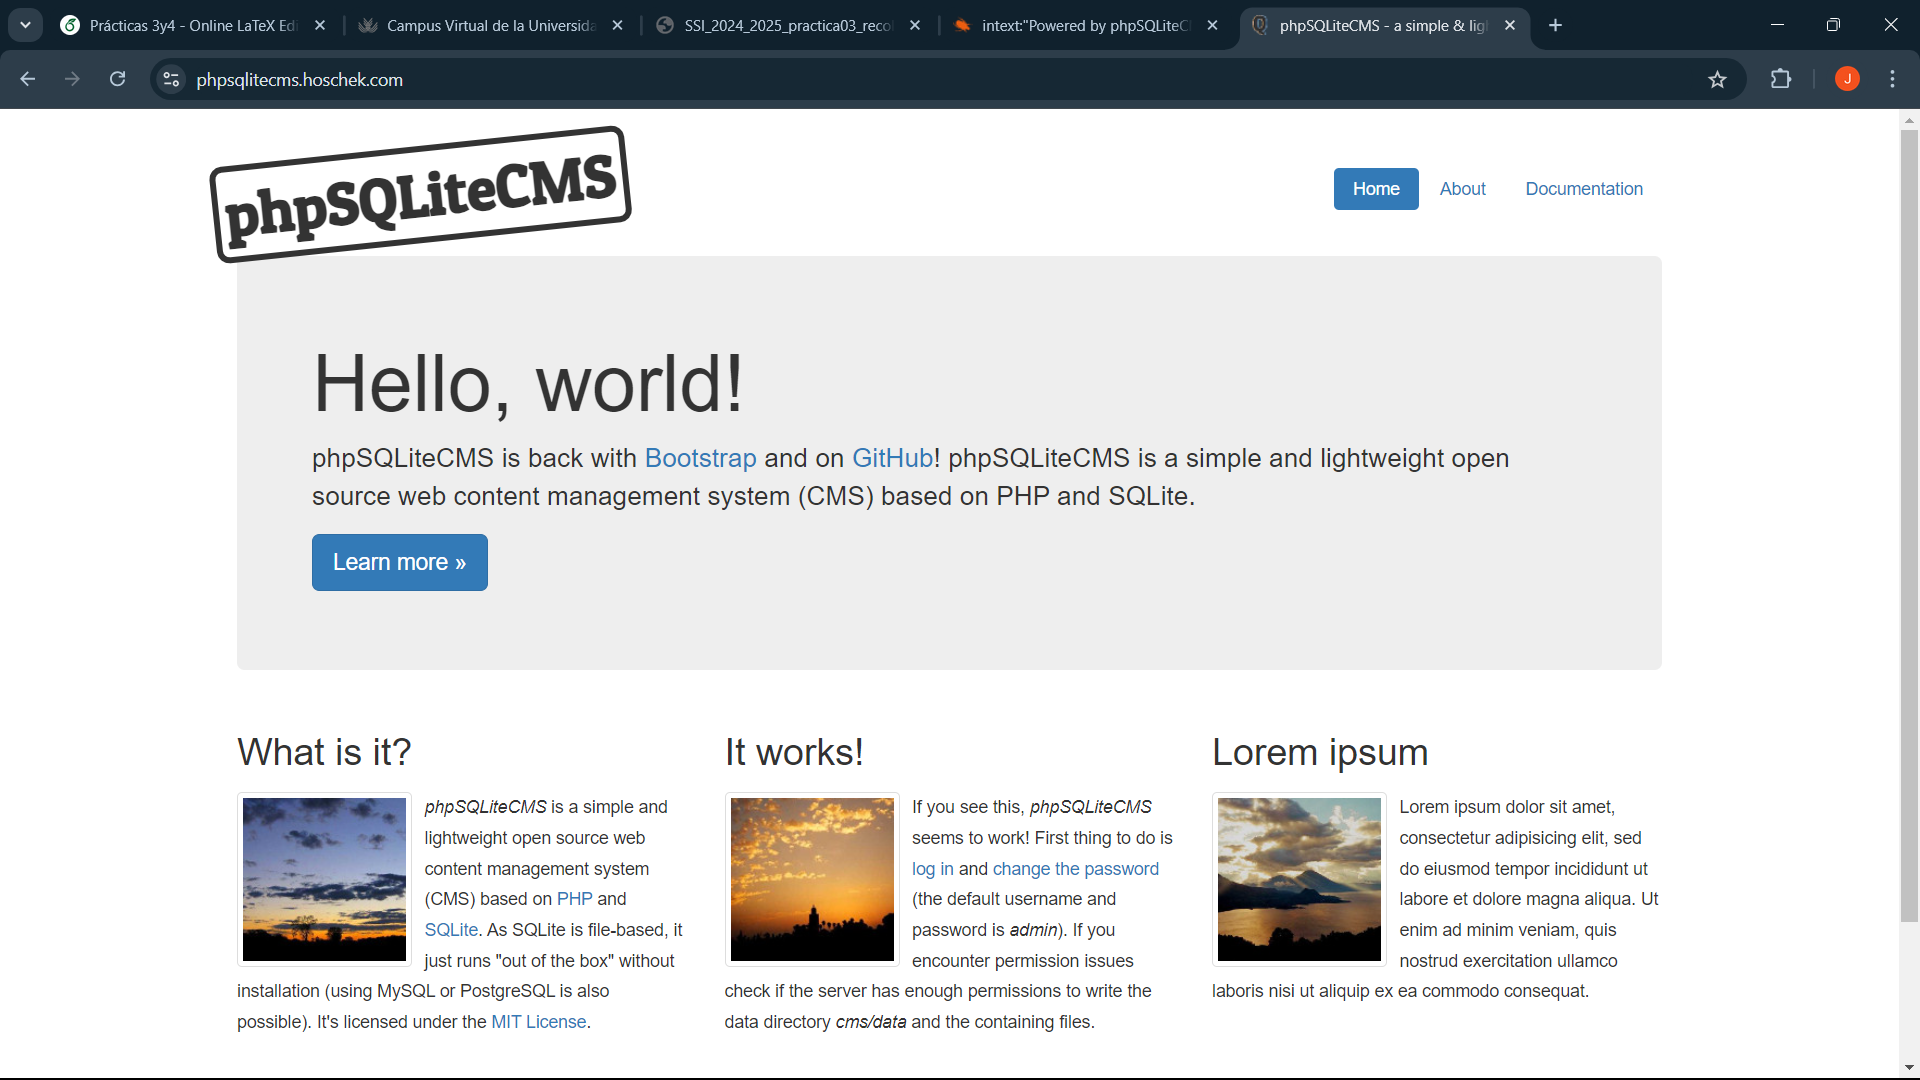
\includegraphics[width=0.5\linewidth]{Practica 3y4/images/Captura de pantalla (83).png}
    \caption{Acceso a uno de los sitios webs}
    \label{fig:enter-label}
\end{figure}
\begin{itemize}
    \item\textit{¿Qué información importante estamos obteniendo a raíz del uso de este dork?}
    Estamos obteniendo distintos sitios webs que usan phpSQLiteCM. phpSQLiteCMS es de código abierto y por tanto, esto permite encontrar algunas vulnerabilidades con mayor facilidad.
\end{itemize}
\newpage
\textit{A continuación, usaremos el dork con título "PHP Credits" "Configuration" "PHP Core" ext:php inurl:info. Haremos clic sobre el enlace con dirección http://61.216.3.97/info.php.
Conteste a las siguientes preguntas:}
\begin{figure}[h]
    \centering
    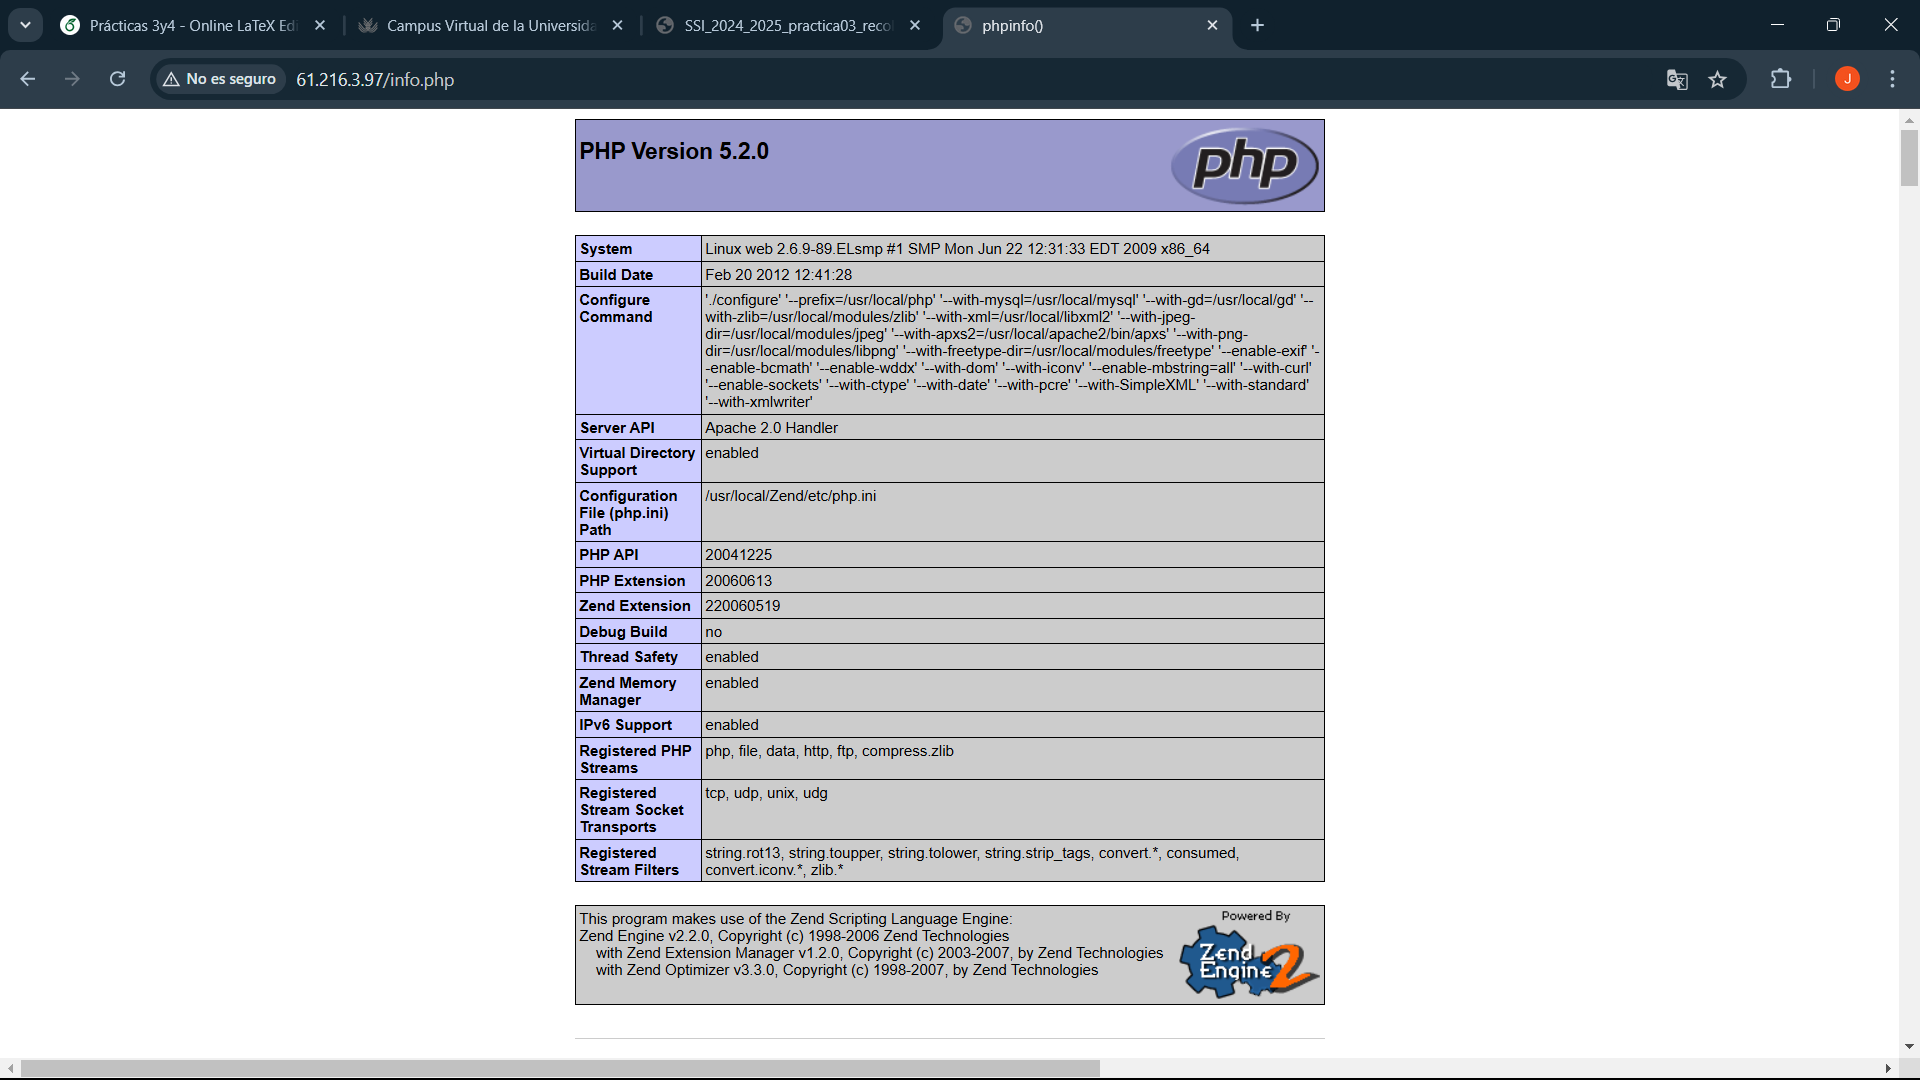
\includegraphics[width=0.5\linewidth]{Practica 3y4/images/Captura de pantalla (84).png}
    \caption{Acceso al sitio web}
    \label{fig:enter-label}
\end{figure}
\begin{itemize}
    \item\textit{¿A qué estamos accediendo exactamente?}\\
    Estamos accediendo a la configurador del servidor PHP 61.216.3.97.
    \item\textit{¿Qué información útil podemos obtener de aquí si nuestras intenciones fueran maliciosas?}\\
    Obtenemos mucha información que podría ser útil desde un punto de vista malicioso, como versión de PHP, esto nos permite buscar las vulnerabilidades conocidas para dicha versión, información acerca del sistema operativo, que igualmente nos ayudaría a encontrar vulnerabilidades para dicha versión de SO, se pueden ver las extensiones de PHP habilitadas (curl, MySQL, etc.), se muestra también la ruta del fichero de configuración inicial (php.ini) y algunas más.\\
    En definitiva al disponer de tanta información sobre la implementación de este servidor, cualquier atacante podría intentar encontrar vulnerabilidades.
\end{itemize}
\newpage
\textit{Finalmente, usaremos el dork cuyo título es: inurl:phpsysinfo/index.php?disp=dynamic. Esto nos devolverá un resultado y accederemos al enlace:\\
http://phpsysinfo.sourceforge.net/phpsysinfo/index. php?disp=dynamic.
Conteste a las siguientes preguntas:}
\begin{figure}[h]
    \centering
    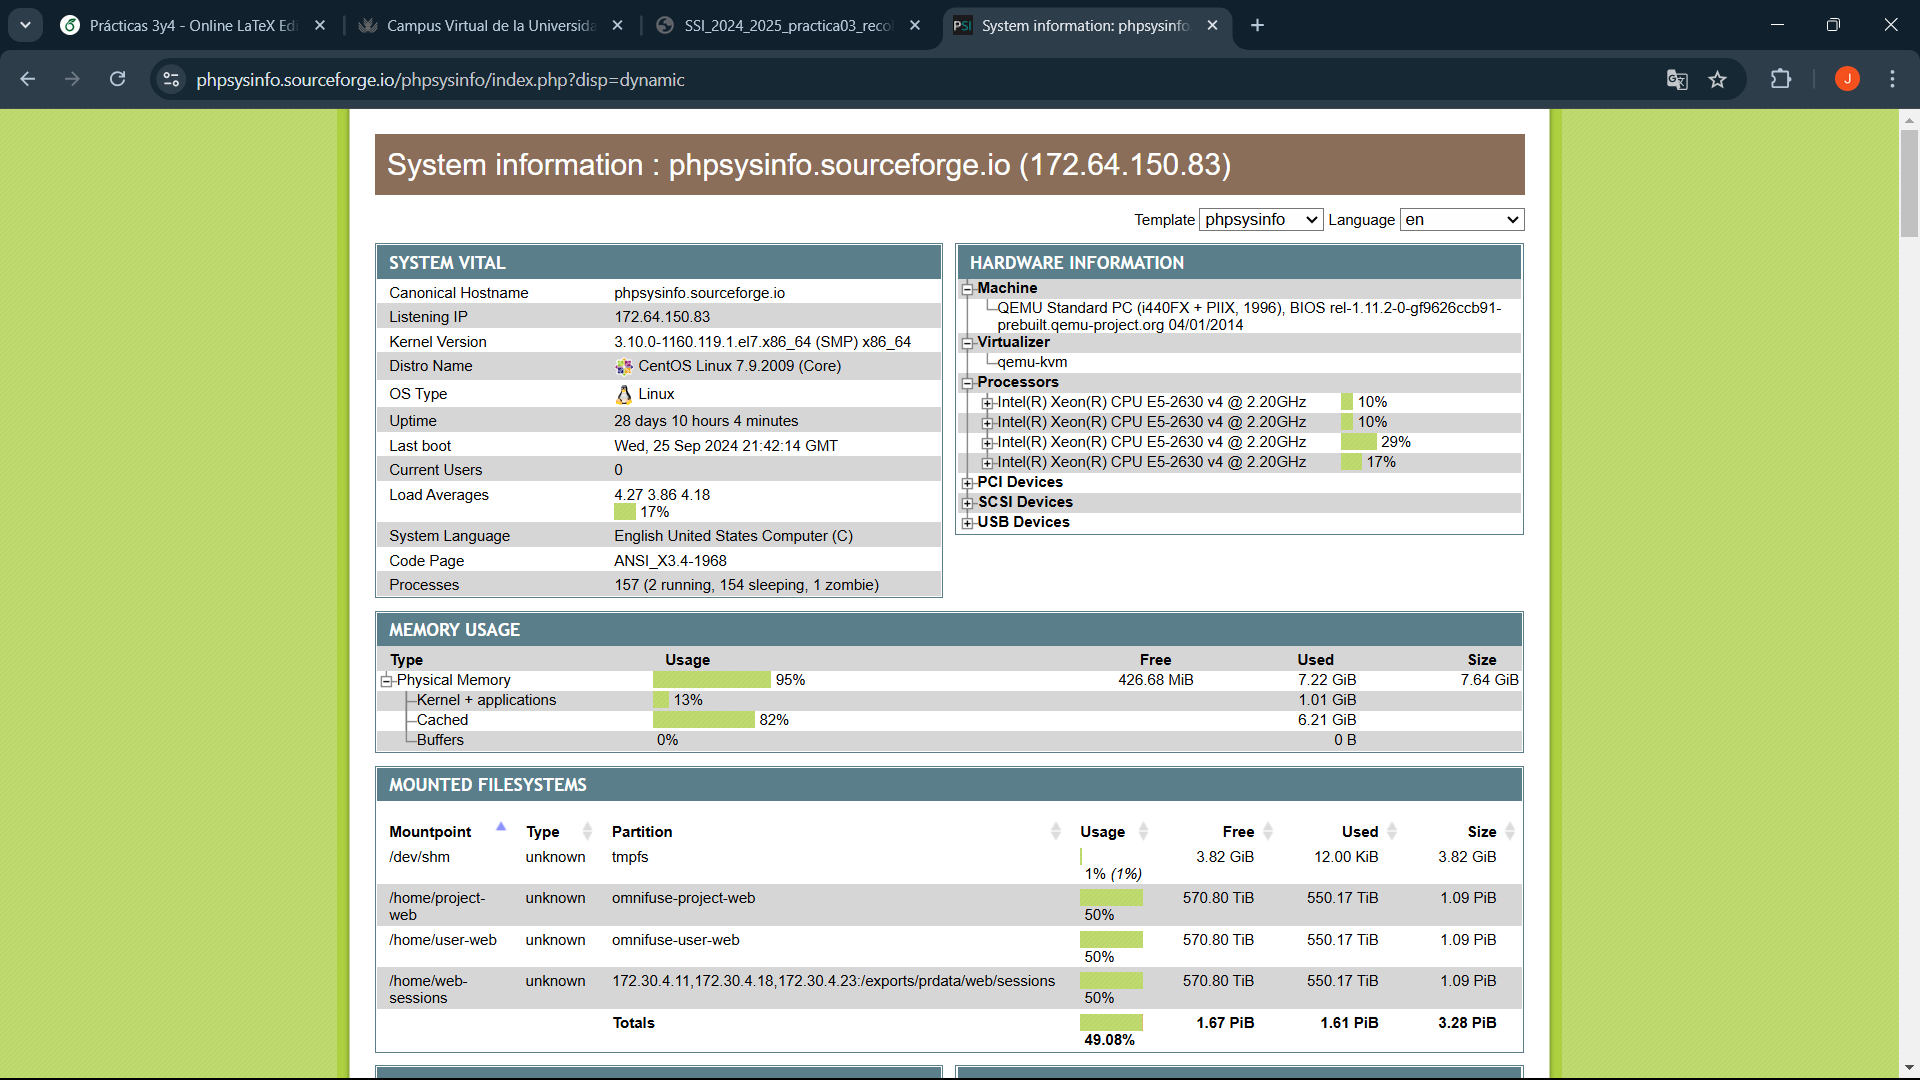
\includegraphics[width=0.5\linewidth]{Practica 3y4/images/Captura de pantalla (85).png}
    \caption{Acceso al sitio web}
    \label{fig:enter-label}
\end{figure}
\begin{itemize}
    \item\textit{¿A qué estamos accediendo exactamente?}\\
    Estamos accediendo a la información del sistema que aloja dicha dirección.
    \item\textit{¿Qué información útil podemos obtener de aquí si nuestras intenciones fueran maliciosas?}\\
    Desde un punto de vista malicioso podemos rescatar bastante información útil, por ejemplo, podemos ver la dirección IP del servidor, información acerca del sistema como el kernel o el SO, el tiempo de actividad (el tiempo que no ha sido reiniciado), procesadores, información acerca de la memoria, entre otras.
    Como en el caso anterior, en definitiva, se muestra demasiada información que puede ser utilizada desde un punto de vista atacante para buscar y explotar vulnerabilidades del sistema.
\end{itemize}

%%%%%%%%%%%%%%%%%%%%%%%%%%%%%%%%%%%%%%%%%%%%%%%%%%%%%%%%%%%%%%%%%%%%%%%%%%%%%%%%%%%%%%%%%
\section{Ejercicio 4}

\textit{Accederemos al enlace cuya URL \url{https://uftm.edu.br/proplan/index.php?option=com_content&view=article&id=110:gtm1-divulgacao-da-uftm&catid=16:cev}.}

\begin{itemize}
    \item \textit{A qué tipo de información estamos accediendo?}
    \newline
    Estamos accediendo a un mensaje de error 'RuntimeException' de una aplicación Joomla.
    \begin{figure}[h]
        \centering
        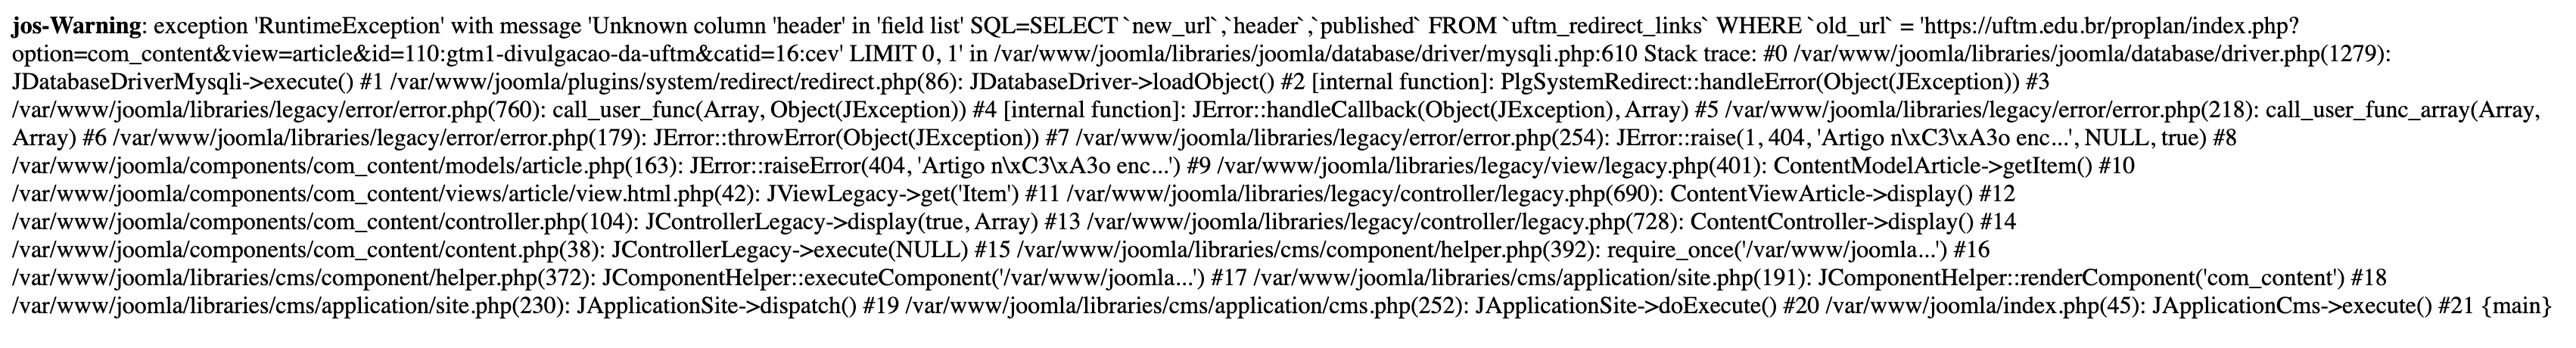
\includegraphics[width=\linewidth]{Practica 3y4/images/Screenshot 2024-10-24 at 10.06.47.png}
        \caption{Código de error al que accedemos.}
        \label{fig:enter-label}
    \end{figure}
    \item \textit{¿Qué información importante obtendríamos de este resultado, si nuestra intención fuera maliciosa?}
    \newline
    Podemos hacer uso de esto para conocer detalles de la base de datos, como por ejemplo, las tablas de la misma, con el fin de conocer la propia estructura de la base de datos y relizar consultas para obtener información sensible.
\end{itemize}

\textit{Ahora, accederemos al enlace con
URL \url{https://eportal.pwc.ca/siteminderagent/forms/smpwservices.fcc.}}
\begin{itemize}
    \item \textit{¿A qué tipo de información estamos accediendo?}
    \newline
    Como podemos ver, estamos accediendo a un panel de información de como deben de ser las contraseñas de ese sitio web.
    \begin{figure}[h]
        \centering
        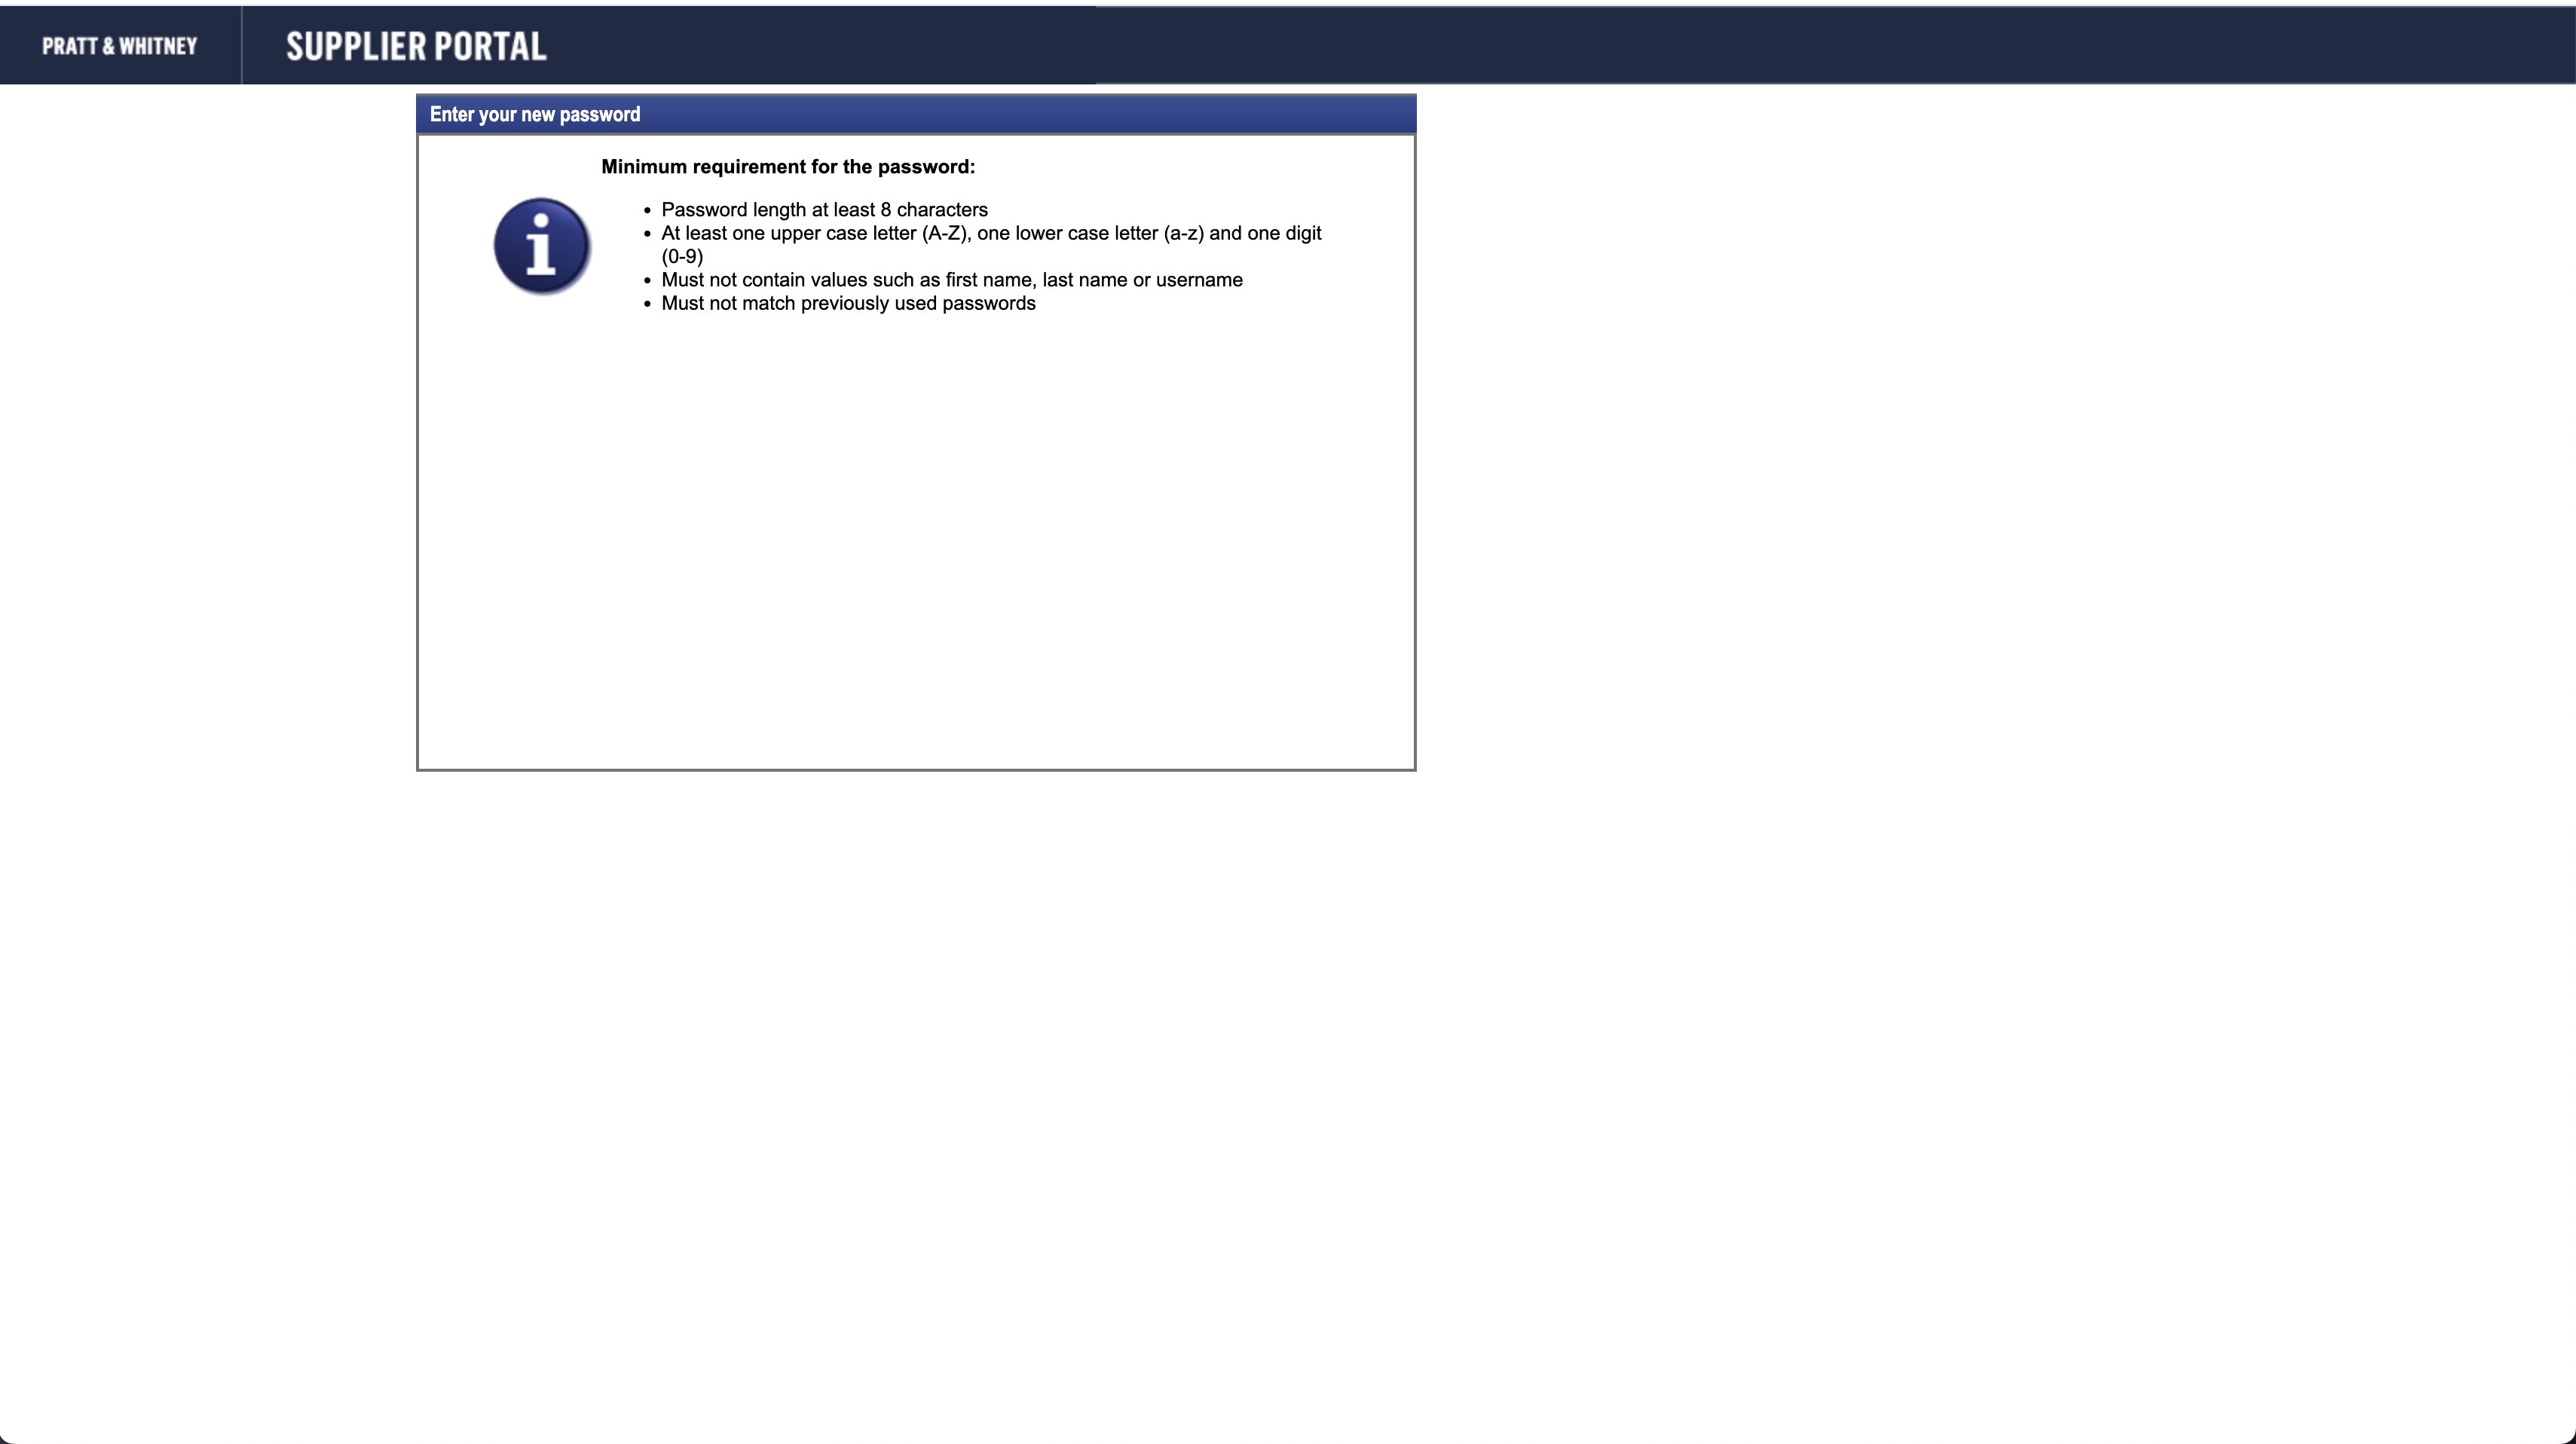
\includegraphics[width=\linewidth]{Practica 3y4/images/Screenshot 2024-10-24 at 10.12.21.png}
        \caption{Panel con información de como debe de ser las contraseñas}
        \label{fig:enter-label}
    \end{figure}
    \item \textit{¿Qué información importante obtendríamos de este resultado, si nuestra intención fuera maliciosa?}
    Podemos saber la composición de las contraseñas de la web, podemos hacer esto para poder filtrar las potenciales contraseñas para realizar un ataque de fuerza bruta y acceder al servicio web.
    \newline
\end{itemize}
%%%%%%%%%%%%%%%%%%%%%%%%%%%%%%%%%%%%%%%%%%%%%%%%%%%%%%%%%%%%%%%%%%%%%%%%%%%%%%%%%%%%%%%%%
\section{Ejercicio 5}

\textit{Vamos a la URL\\ \url{https://www.jeeptelevision.com/fotoeventi/index.php?folder=c2ljaWxpYQ==}}

\begin{itemize}
    \item \textit{¿A qué nos da acceso dicho enlace?}
    \newline
    Al sistema de ficheros de una máquina (directorio /home).
    \begin{figure}[h]
        \centering
        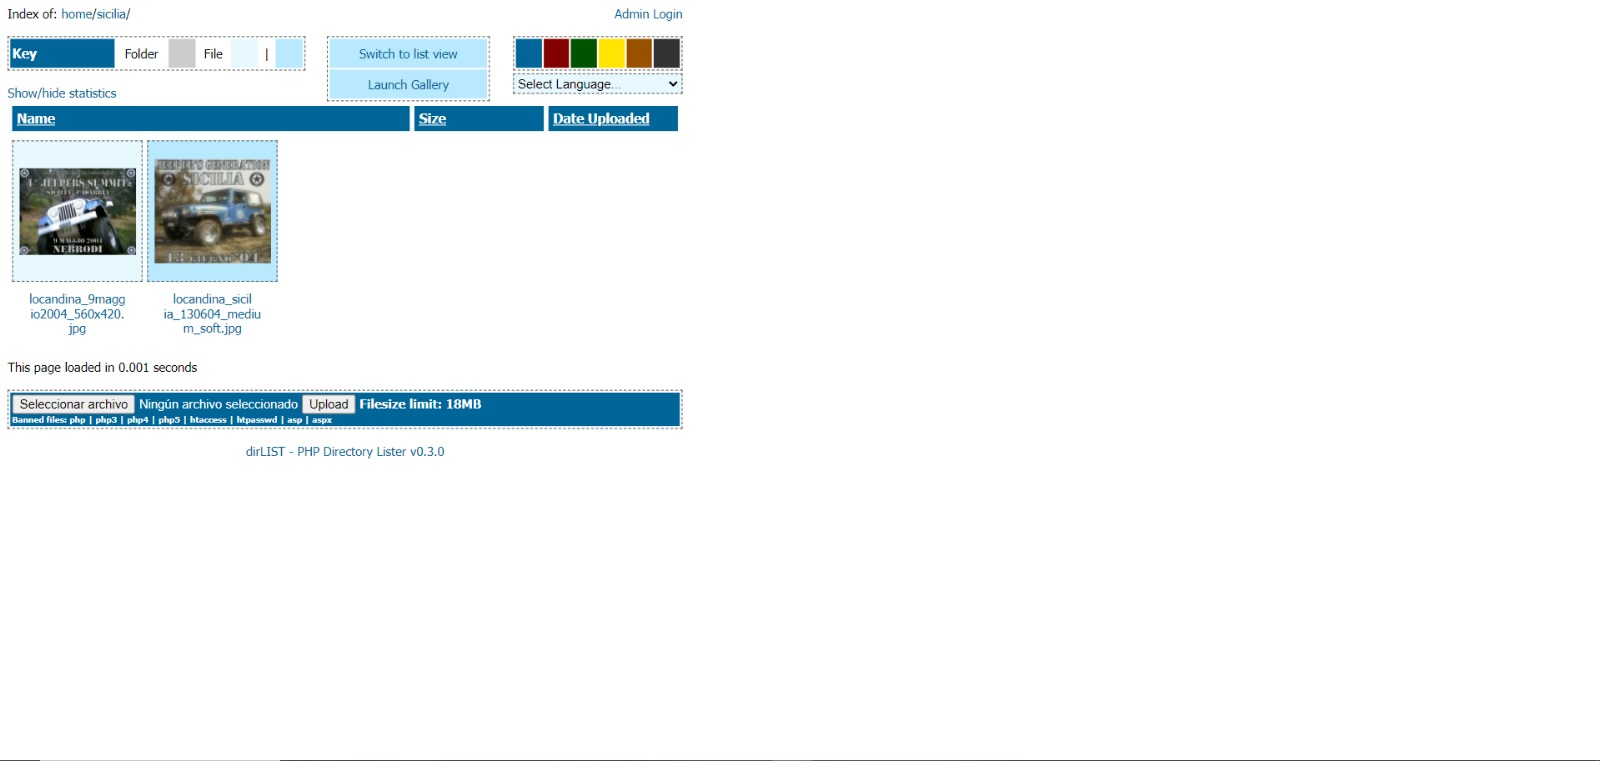
\includegraphics[width=\linewidth]{Practica 3y4/images/WhatsApp Image 2024-10-24 at 10.19.57.jpeg}
        \caption{Directorio /home de un servidor.}
        \label{fig:enter-label}
    \end{figure}
    \item \textit{¿Qué acciones podemos realizar usando este enlace?}
    \newline
    Tener acceso a la información del sistema, modificar y subir archivos.
    \begin{figure}[h]
        \centering
        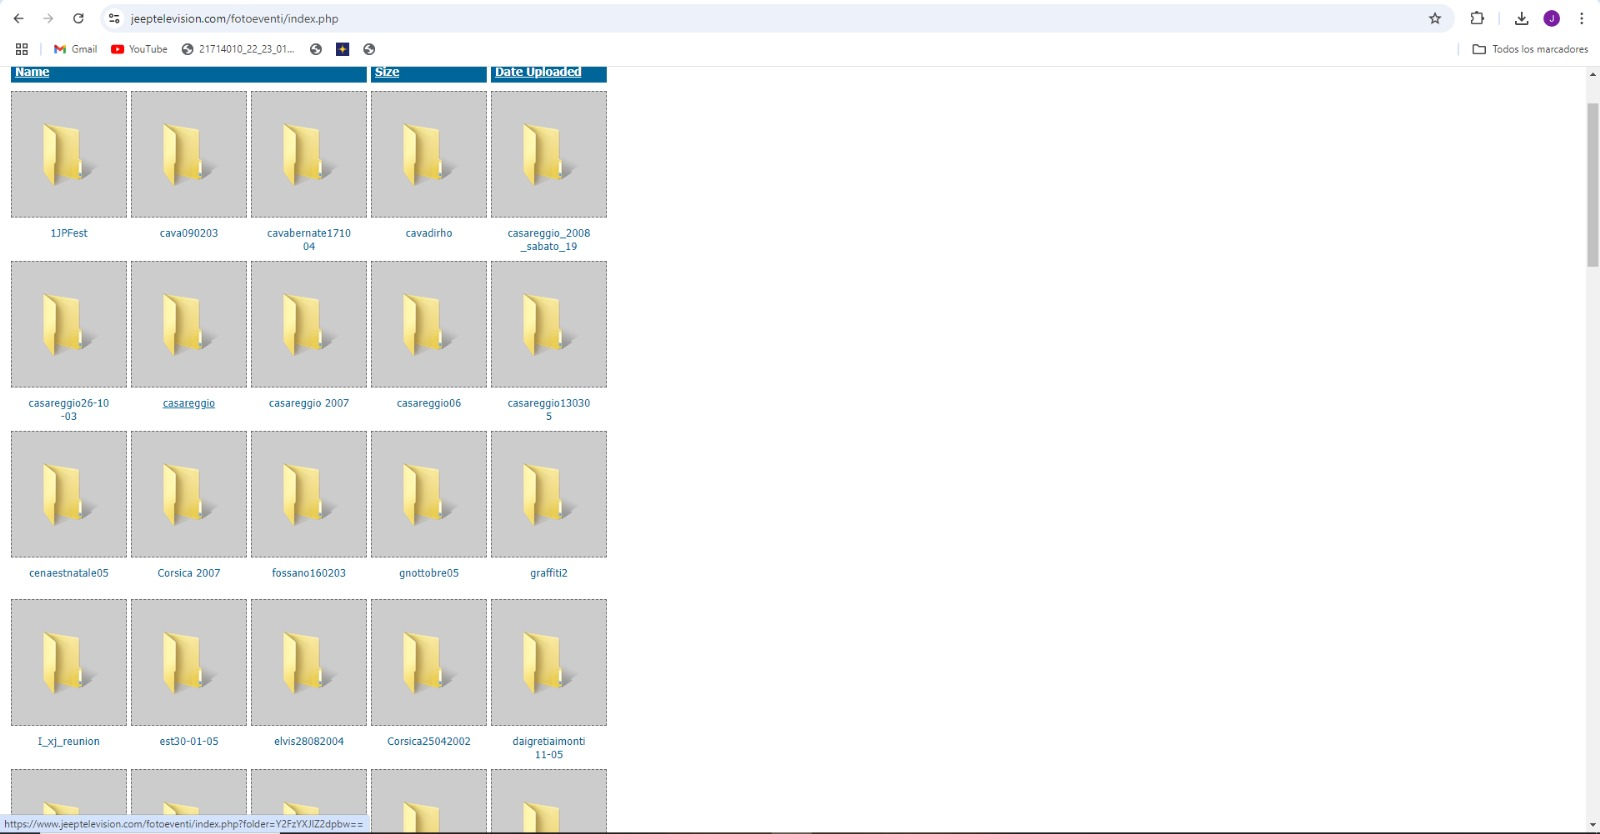
\includegraphics[width=0.5\linewidth]{Practica 3y4/images/WhatsApp Image 2024-10-24 at 10.20.22.jpeg}
        \caption{Caption}
        \label{fig:enter-label}
    \end{figure}
    \item \textit{Desde el punto de vista de un ataque malicioso, ¿cómo podríamos sacar partido de este enlace?}
    \newline
    El simple hecho de tener acceso a los archivos puede resultar un ataque si se tratase de información confidencial, también podríamos modificar los archivos sin estar autorizados e incluso subir archivos maliciosos al sistema.    
\end{itemize}

%%%%%%%%%%%%%%%%%%%%%%%%%%%%%%%%%%%%%%%%%%%%%%%%%%%%%%%%%%%%%%%%%%%%%%%%%%%%%%%%%%%%%%%%%
\section{Ejercicio 6}
\textit{
De los dorks que encontramos en el enlace usaremos dos, el primero será el que tiene como título allinurl: drive.Google.com/open?id=.Con este tipo de dork podríamos acceder, por ejemplo, al enlace
con URL:\\
https://drive.google.com/file/d/0ByO02CwASGN0d0hNbWM4OEc5ZmM/view?resourcekey=0-OrCfpNOoo9q7fbXmsMIHQQ.\\
Conteste a las siguientes preguntas:
}
 \begin{figure}[h]
        \centering
        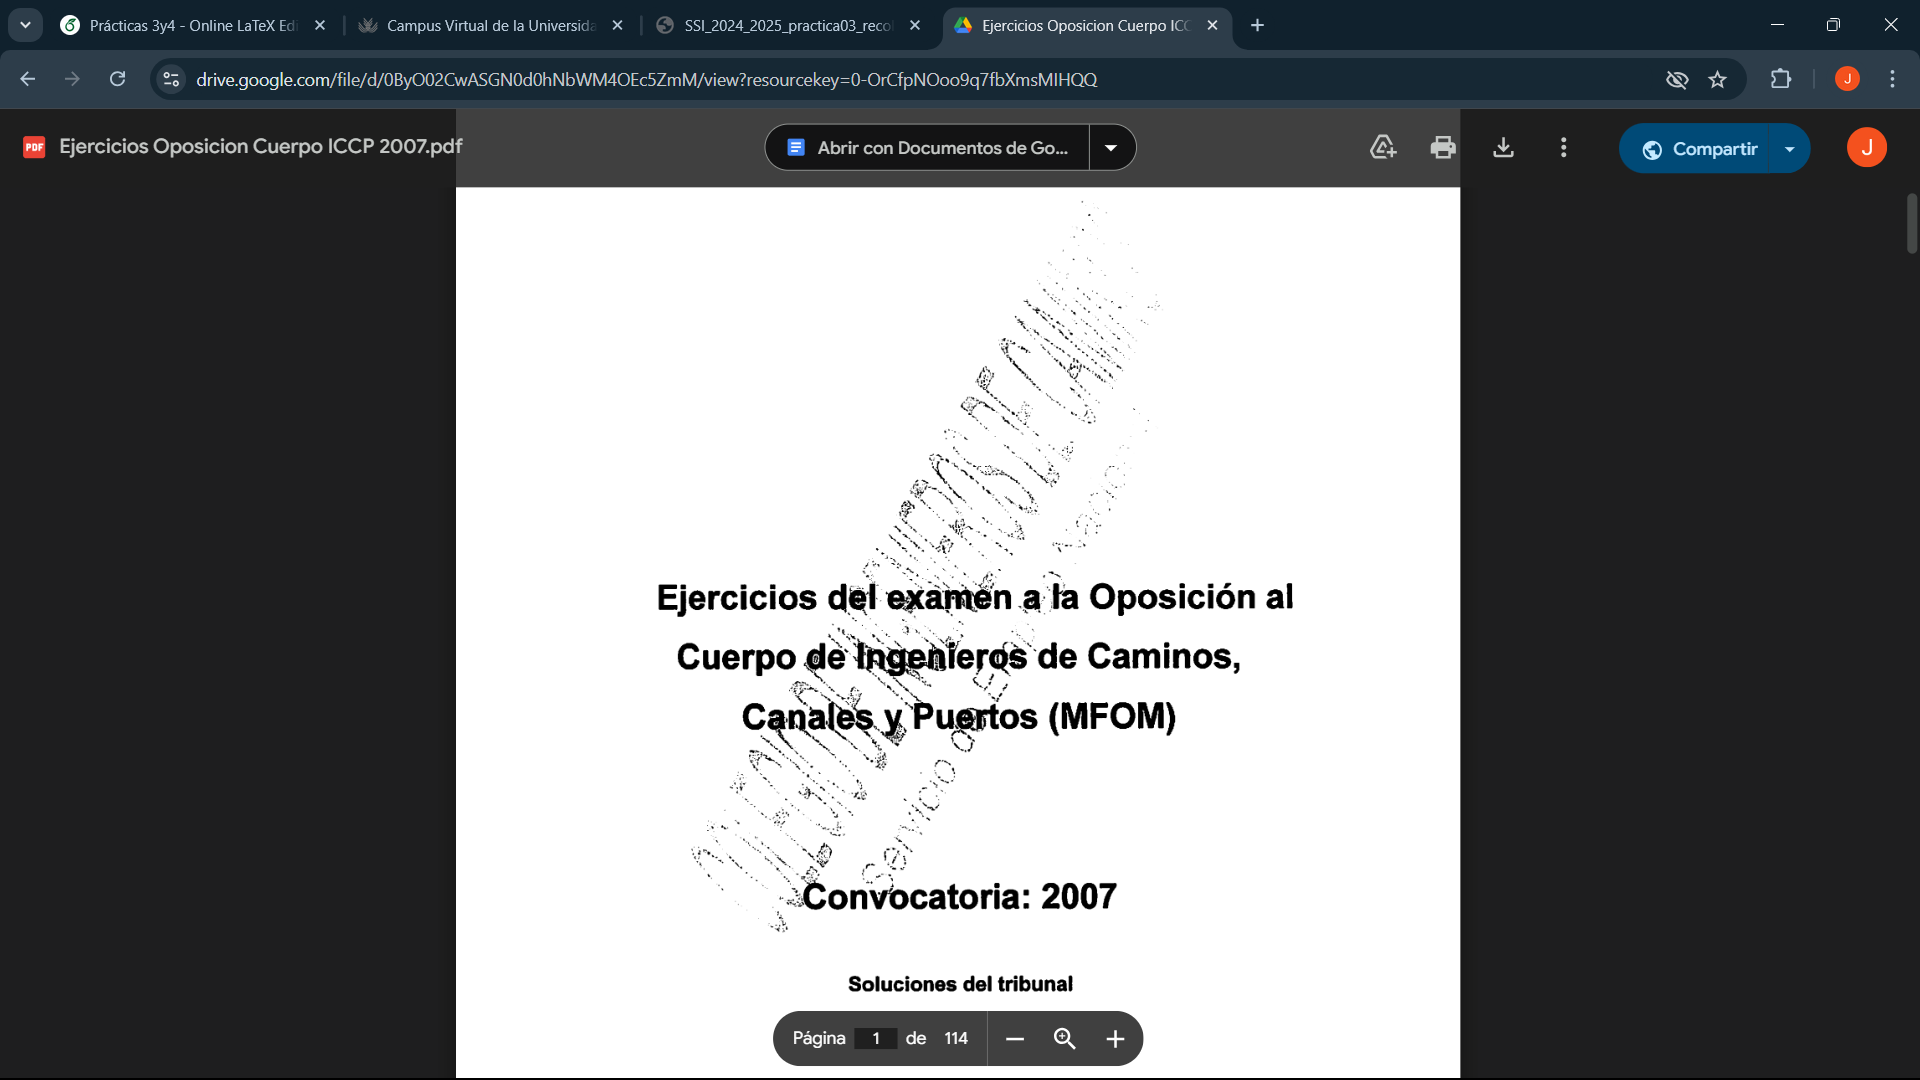
\includegraphics[width=0.5\linewidth]{Practica 3y4/images/Captura de pantalla (86).png}
        \caption{Captura del sitio encontrado}
        \label{fig:enter-label}
\end{figure}
\begin{itemize}
    \item \textit{Exactamente, ¿a qué estamos accediendo?}\\
        Como podemos observar estamos accediendo al solucionario del examen de oposición del Cuerpo de Ingenieros de Caminos, Canales y Puertos de 2007.
    \item \textit{¿Qué utilidad podemos encontrarle a este dork?}\\
        Podemos encontrar ejercicios resueltos para estudiar para una convocatoria actual, o tratar de buscar otros exámenes más recientes de la misma manera que hemos encontrado este.
\end{itemize}
\newpage
\textit{A continuación, usaremos el dork cuyo título es filetype:txt ‘‘gmail’’ | ‘‘hotmail’’ | ‘‘yahoo’’ -robots site:gov | site:us. Accederemos al enlace:\\
https://www.sec.gov/Archives/edgar/data/921669/000092847508000248/dfan14a070708.
txt.\\
Conteste a las siguientes preguntas:}\\

\begin{figure}[h]
    \centering
    \begin{minipage}{0.45\textwidth}
        \centering
        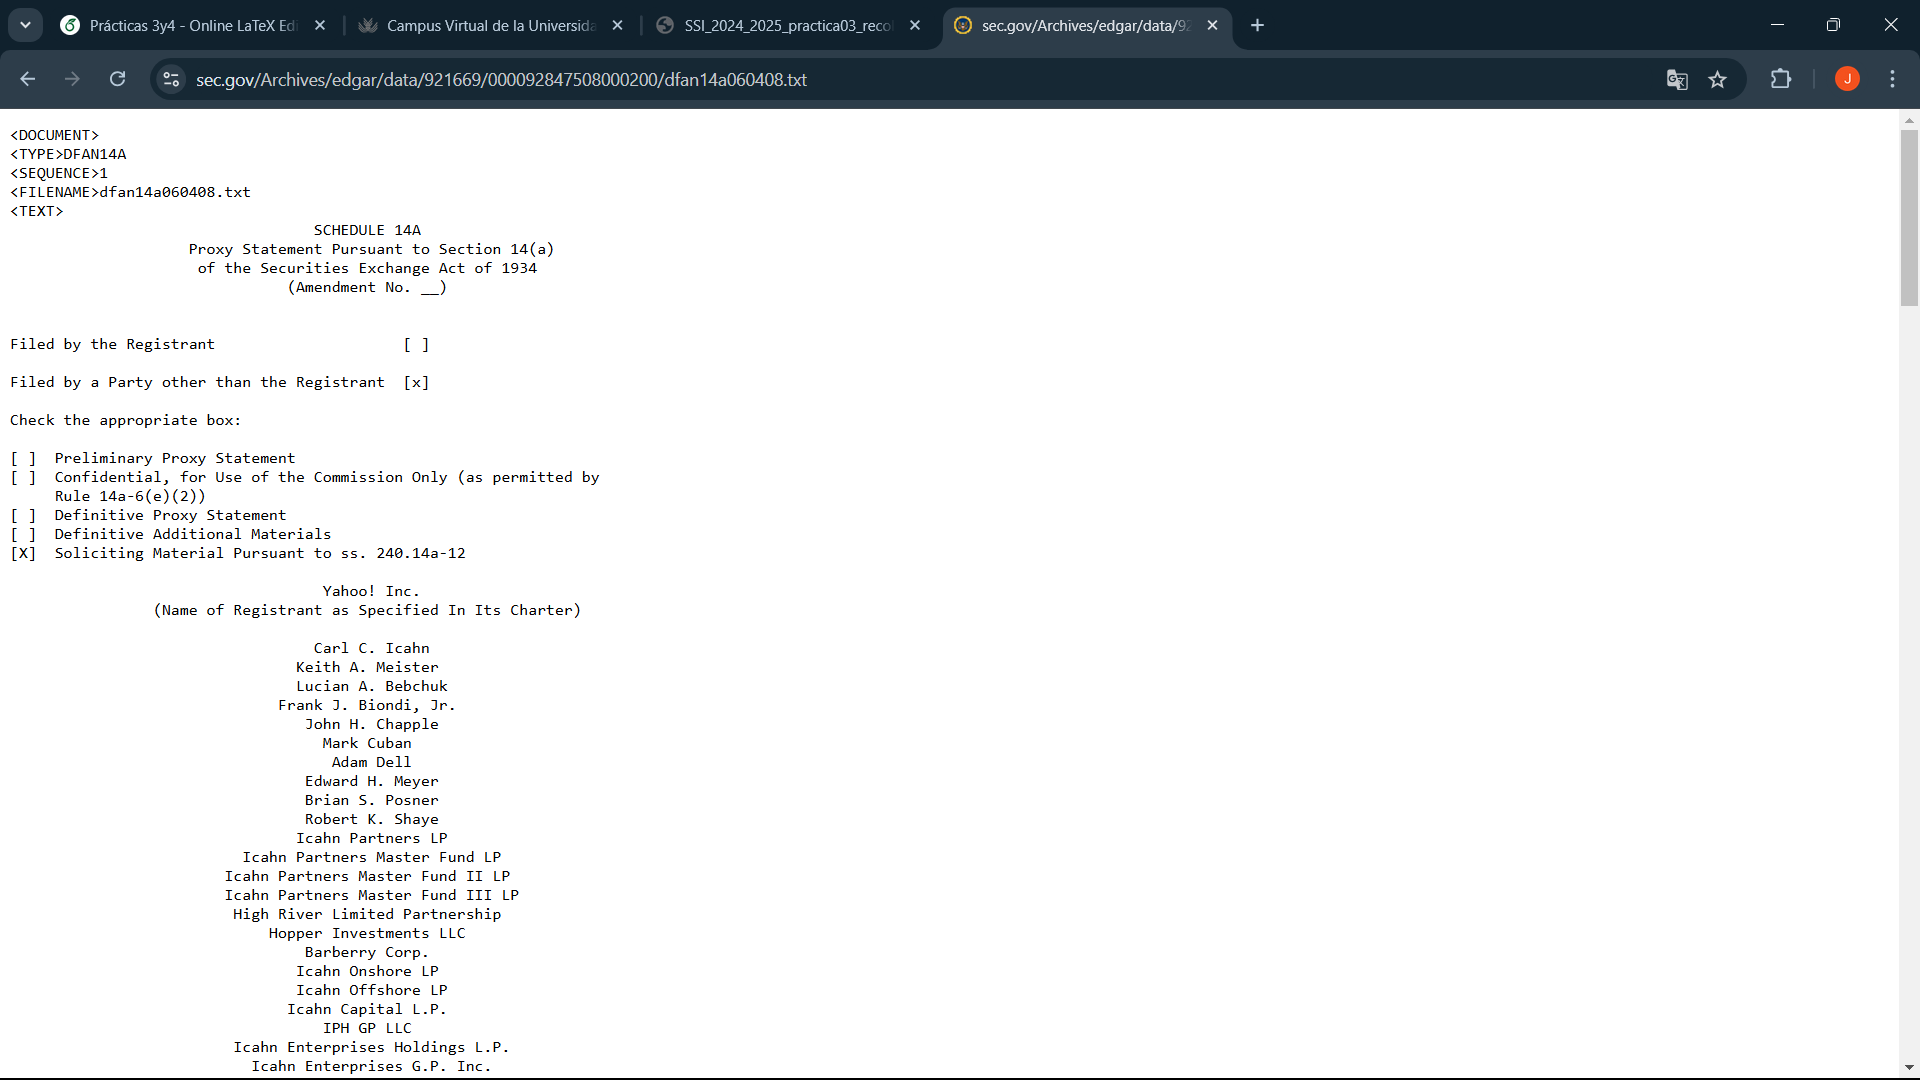
\includegraphics[width=\textwidth]{Practica 3y4/images/Captura de pantalla (87).png}
    \end{minipage}\hfill
    \begin{minipage}{0.45\textwidth}
        \centering
        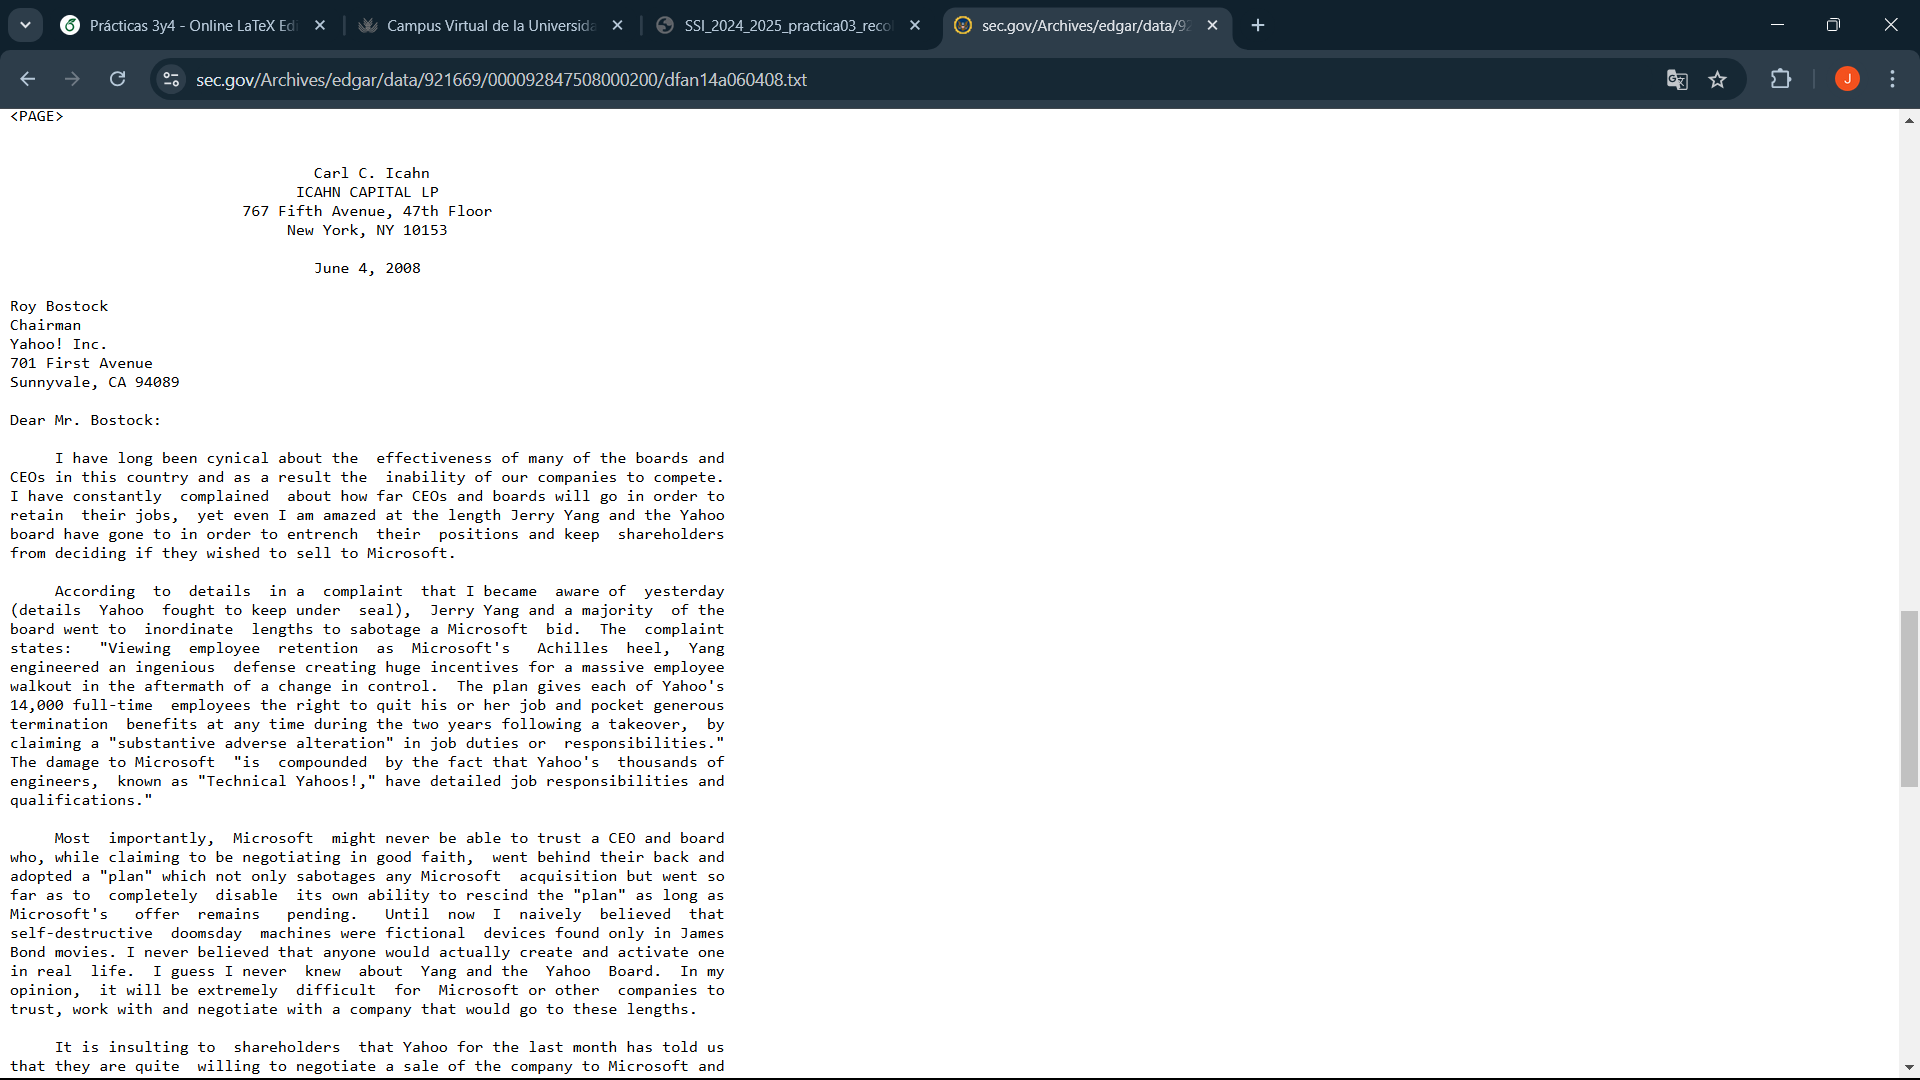
\includegraphics[width=\textwidth]{Practica 3y4/images/Captura de pantalla (90).png}
    \end{minipage}
    \caption{Imágenes del proxy statement}
\end{figure}

\begin{itemize}
    \item \textit{¿Qué estamos viendo?}\\
        Estamos viendo un \textit{"proxy statement"}~\cite{ProxyStatement} de Carl C.Icahn, en este Carl C.Icahn discute por cambios en la junta directiva de \textit{"Yahoo!"}
        
    \item \textit{¿Qué información útil podemos obtener de este enlace?}\\
        Podemos sacar información interna de la organización y las estrategias que se van a seguir.
    \item \textit{¿Por qué podríamos considerar esta información sensible?}\\
        Por el mismo motivo que en la pregunta anterior, se puede sacar información interna la cual puede afectar negativamente a la empresa ya sea por revelación de decisiones privadas, pérdida de la confianza en dicha empresa, etc. estas acciones pueden hacer que el valor de la empresa disminuya gravemente. También otras empresas competidoras con dicha información pueden aprovecharla para fortalecerse y superar a \textit{Yahoo!}.        
\end{itemize}
%%%%%%%%%%%%%%%%%%%%%%%%%%%%%%%%%%%%%%%%%%%%%%%%%%%%%%%%%%%%%%%%%%%%%%%%%%%%%%%%%%%%%%%%%
\newpage
\section{Ejercicio 7}
\textit{Haciendo uso de dorks de Shodan, encuentre las IP correspondientes a 2 equipos con servicio MQTT (Message Queuing Telemetry Transport) en la ciudad de Logroño de la organización “arsys.es”.}

Hacemos uso de los parámetros: \textbf{org}, \textbf{country}, \textbf{city}, para especificar la empresa, el país y la ciudad a donde buscar, respectivamente.
\begin{figure}[h]
    \centering
    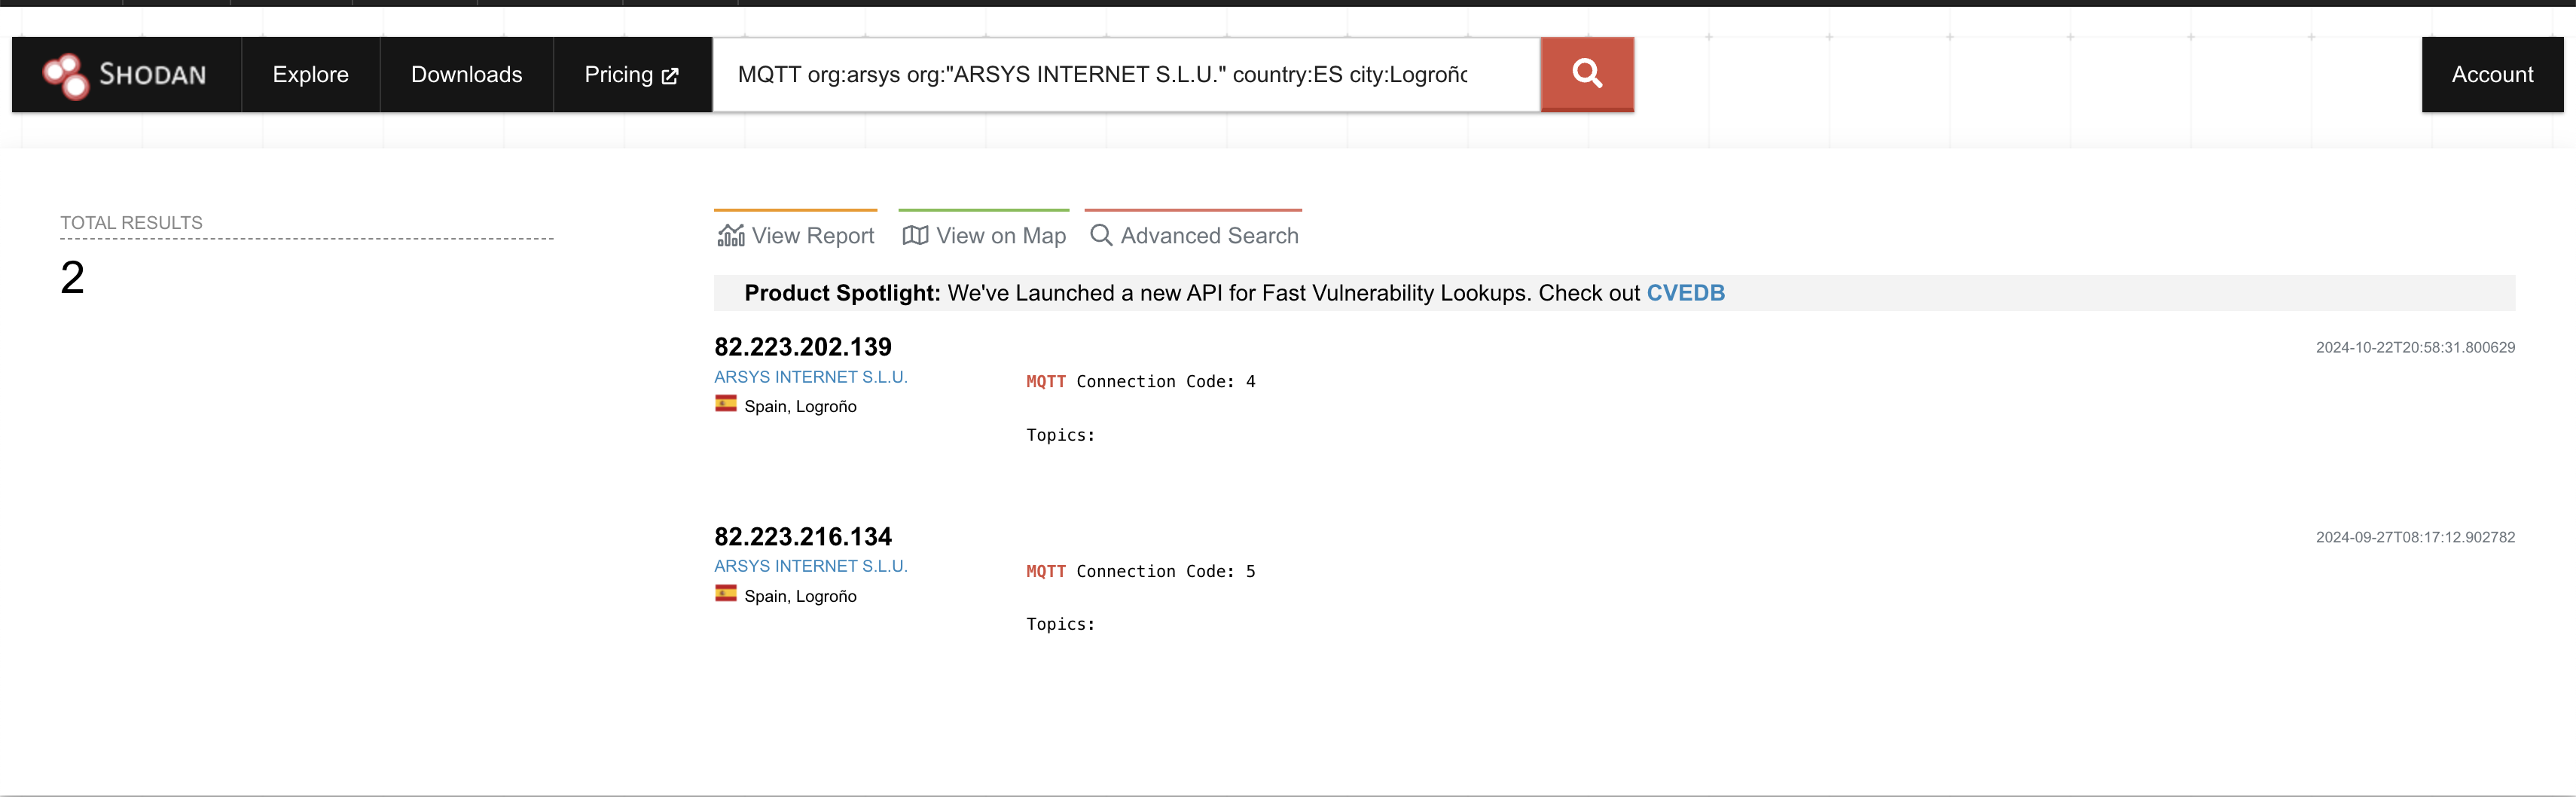
\includegraphics[width=\linewidth]{Practica 3y4/images/Screenshot 2024-10-24 at 10.28.43.png}
    \caption{Búsqueda en Shodan.}
    \label{fig:enter-label}
\end{figure}
%%%%%%%%%%%%%%%%%%%%%%%%%%%%%%%%%%%%%%%%%%%%%%%%%%%%%%%%%%%%%%%%%%%%%%%%%%%%%%%%%%%%%%%%%
\newpage
\section{Ejercicio 8}
\textit{Haciendo uso de Shodan, encuentre el número de equipos del Nuclear Physics Institute de Moscu con el puerto Telnet a la escucha.}
\begin{figure}[h]
    \centering
    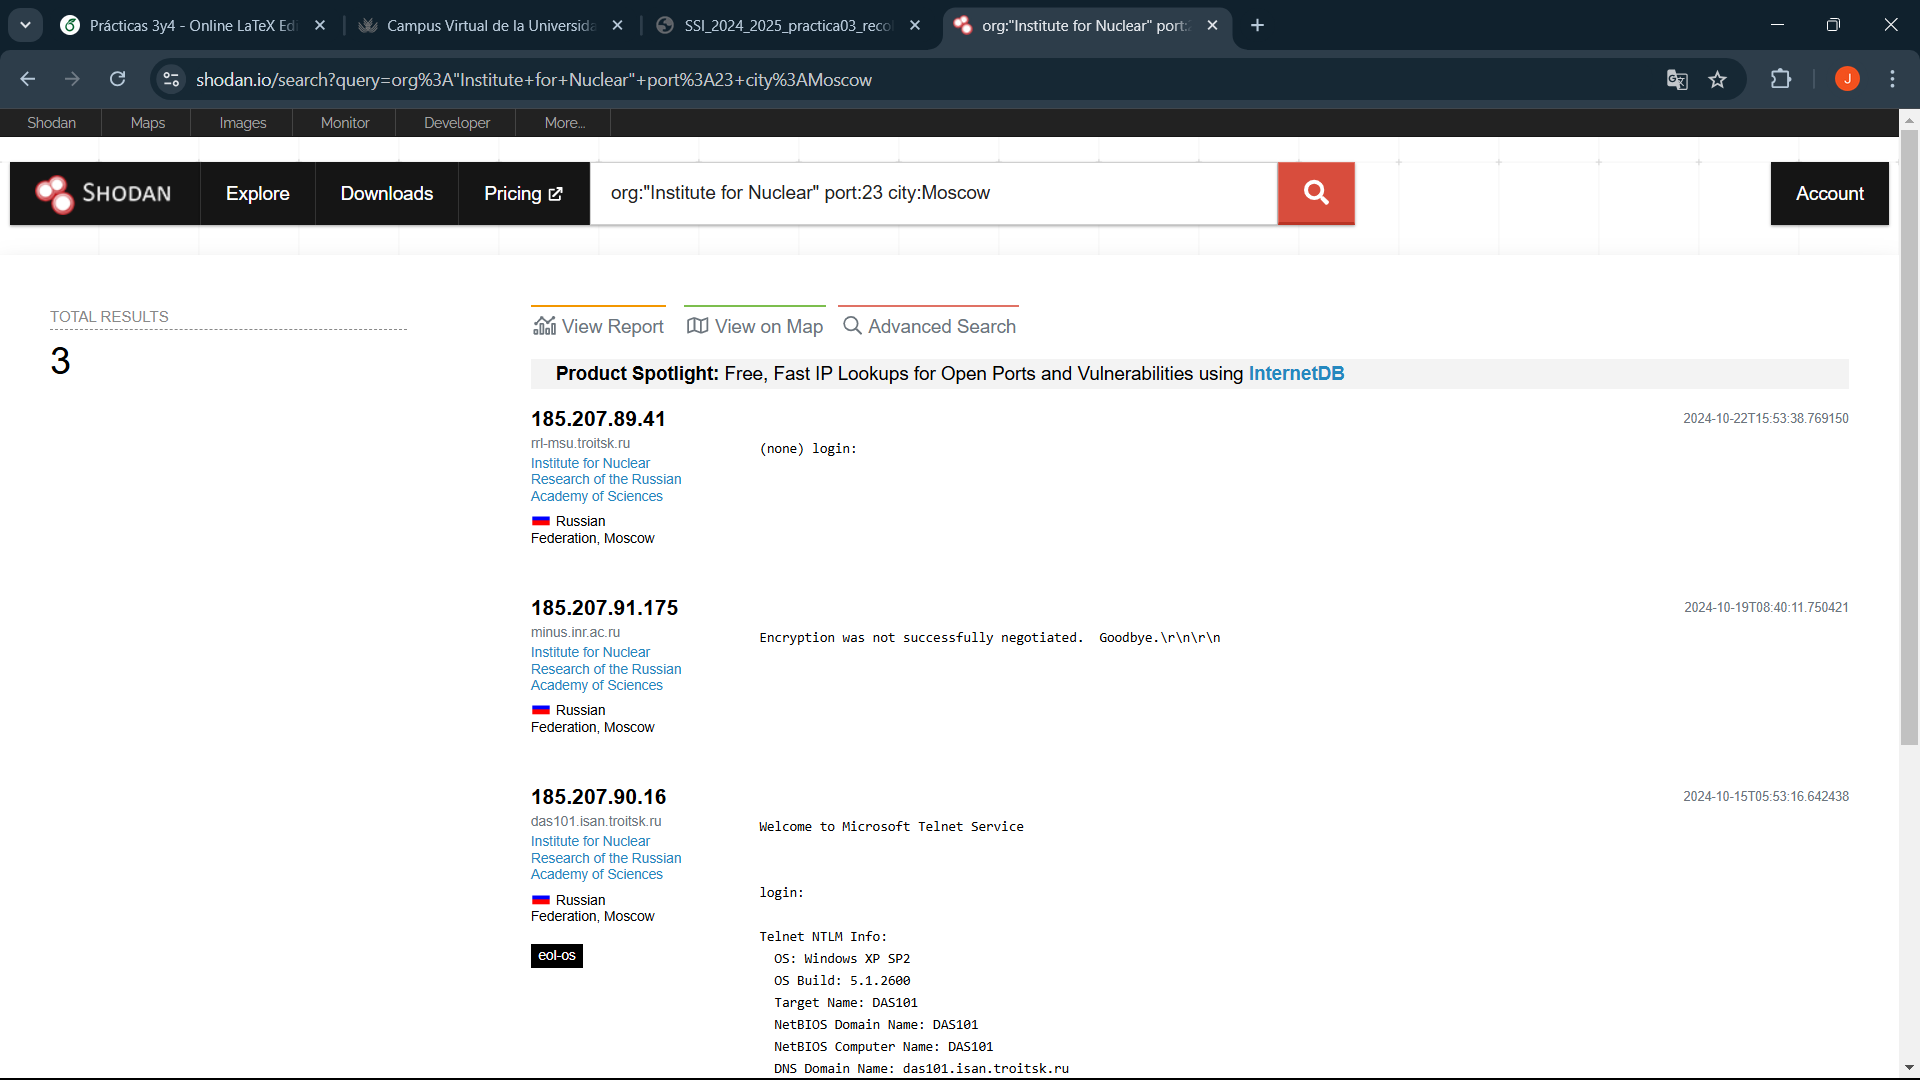
\includegraphics[width=\linewidth]{Practica 3y4/images/Captura de pantalla (93).png}
    \caption{Búsqueda del Institute for Nuclear Research de Moscú con el puerto Telnet a la escucha}
    \label{fig:enter-label}
\end{figure}

%%%%%%%%%%%%%%%%%%%%%%%%%%%%%%%%%%%%%%%%%%%%%%%%%%%%%%%%%%%%%%%%%%%%%%%%%%%%%%%%%%%%%%%%%
\section{Ejercicio 9}
\textit{Haciendo uso de Shodan, encuentre el nombre de la organización que más servidores de Minecraft hostea en la actualidad. Una vez hecho esto encuentre la IP de los servidores de este conocido juego en la provincia de Sevilla.}
\newline
El nombre de la organización que más servidores de Minecraft hostea es BisectHosting con un total de 11500 servidores.
\begin{figure}[h]
    \centering
    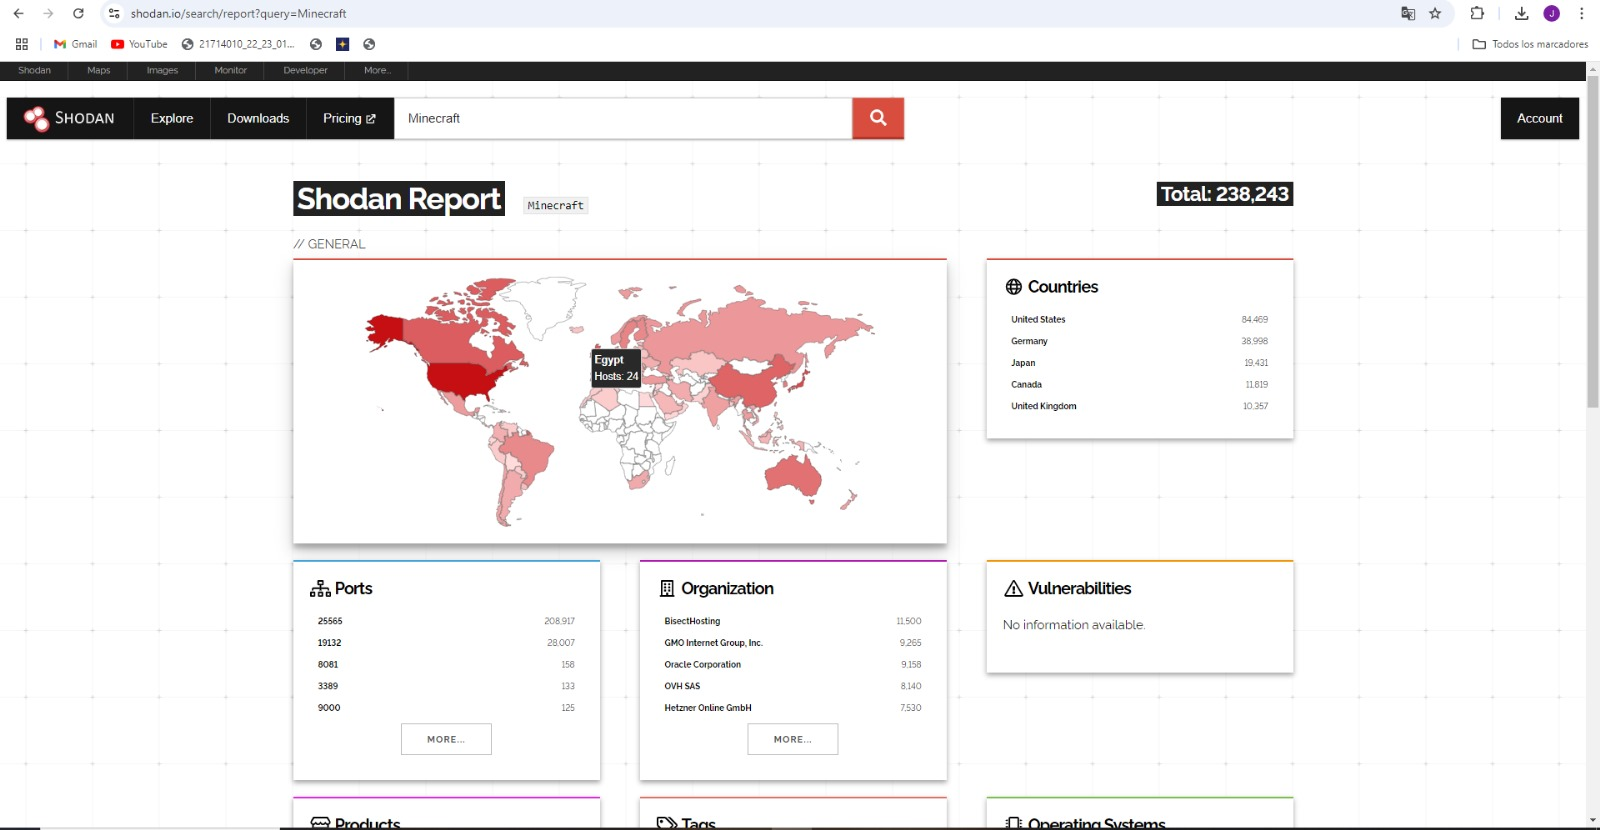
\includegraphics[width=.7\linewidth]{Practica 3y4/images/WhatsApp Image 2024-10-24 at 10.48.04.jpeg}
    \caption{Búsqueda de la organización con más servidores.}
    \label{fig:enter-label}
\end{figure}

La IPs de las organizaciones con sevidores de Minecraft de Sevilla son:

\begin{figure}[h]
    \centering
    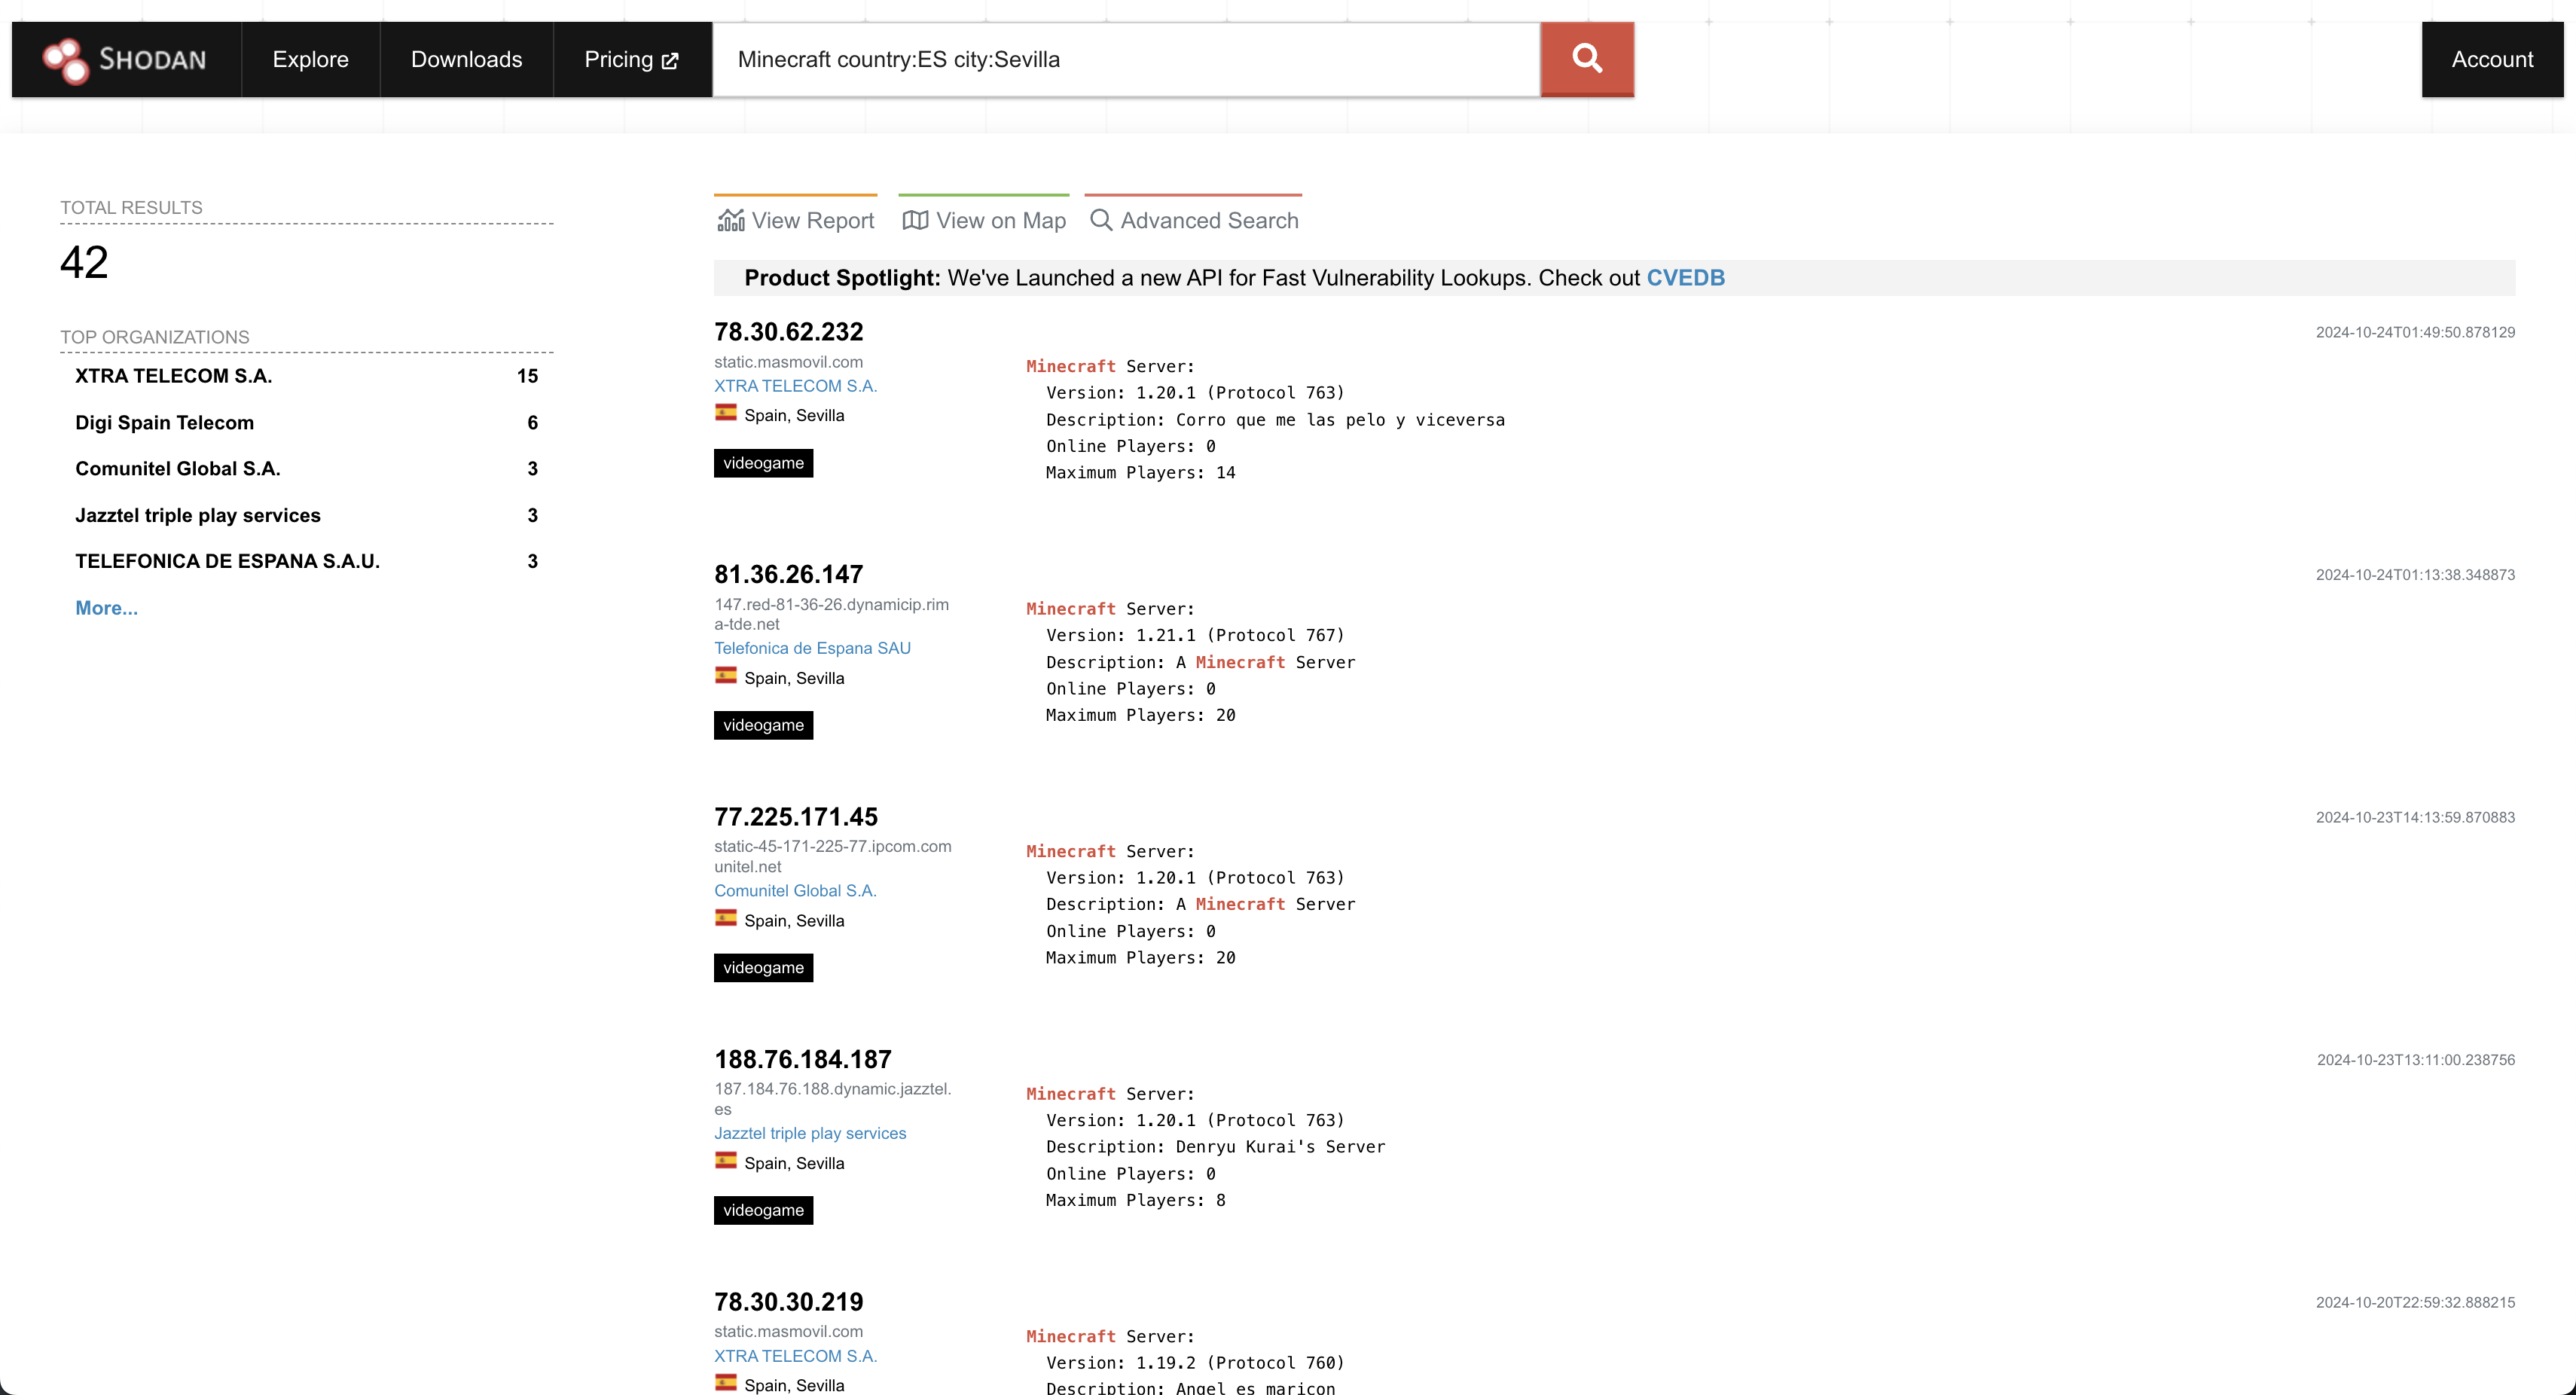
\includegraphics[width=.7\linewidth]{Practica 3y4/images/Screenshot 2024-10-24 at 10.52.06.png}
    \caption{Busqueda en Shodan I}
    \label{fig:enter-label}
\end{figure}
\newpage
\begin{figure}[h]
    \centering
    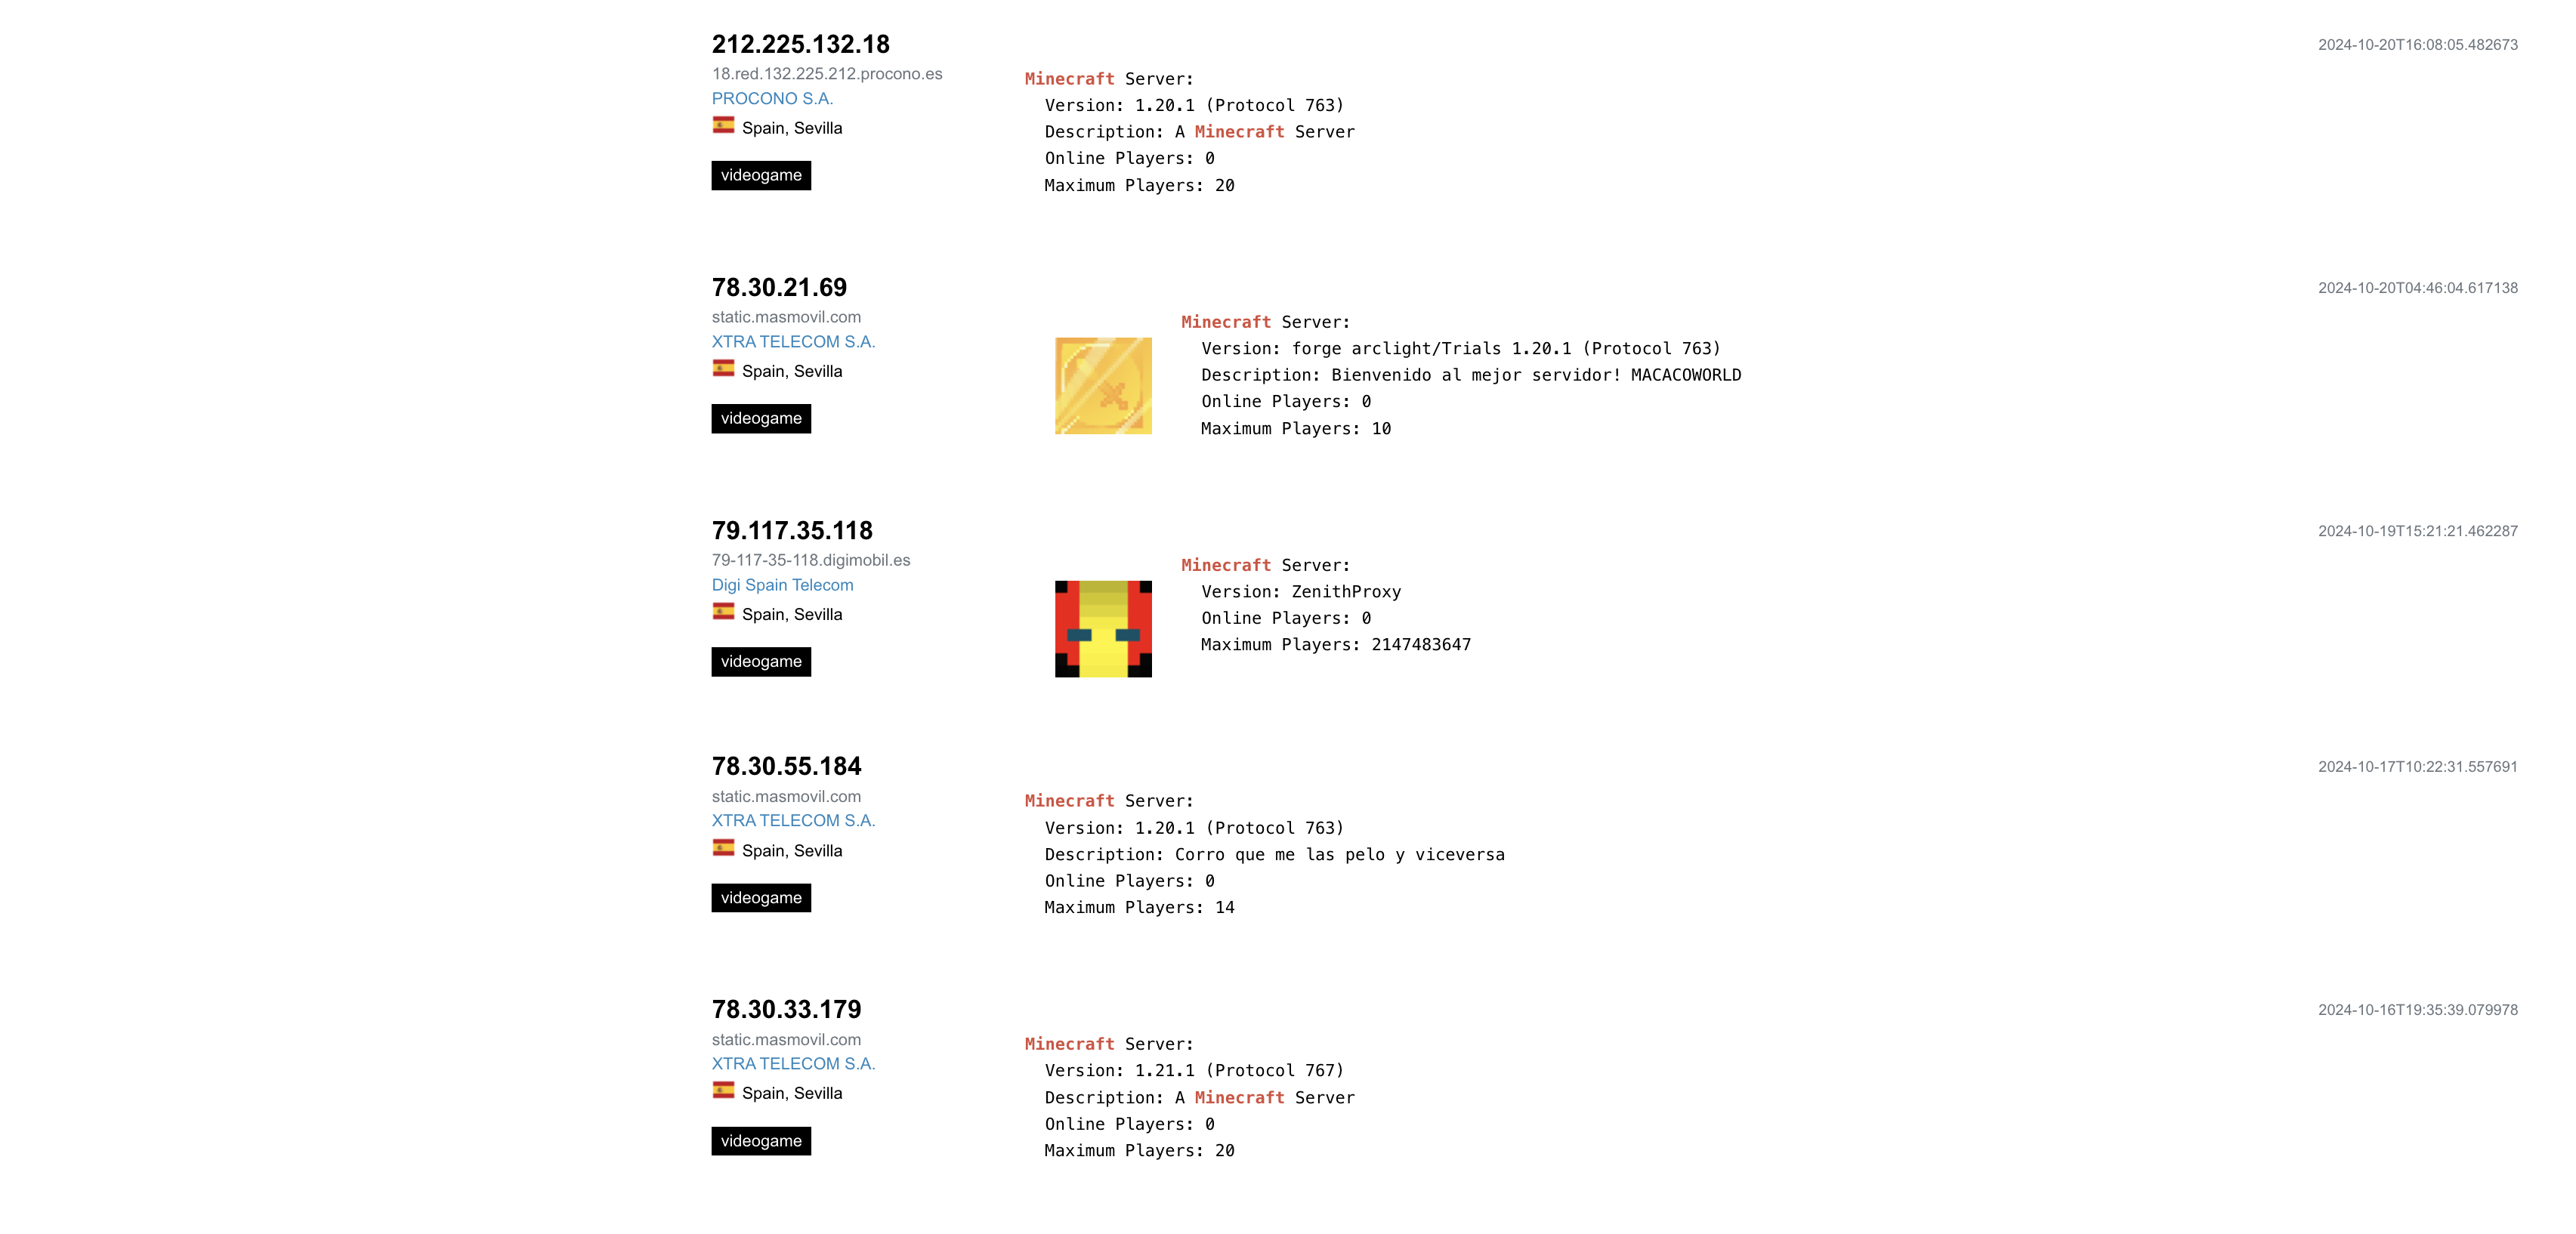
\includegraphics[width=.7\linewidth]{Practica 3y4/images/Screenshot 2024-10-24 at 10.52.16.png}
    \caption{Búsqueda en Shodan II}
    \label{fig:enter-label}
\end{figure}

%%%%%%%%%%%%%%%%%%%%%%%%%%%%%%%%%%%%%%%%%%%%%%%%%%%%%%%%%%%%%%%%%%%%%%%%%%%%%%%%%%%%%%%%%
\chapter{Práctica 3.2: Recolección de información en fuentes abiertas II}

\section{Ejercicio 1}
\textit{Usando DNSDumpster~\cite{DNSDumpster} haga un análisis de los subdominios de cadiz.es}
\begin{itemize}
    \item \textit{¿Qué ISP aloja la mayoría de las webs?}
    \newline
    El \textit{ISP} que más se usa es el denominado \textbf{ACENS\_AS}:
    \begin{figure}[h]
    \begin{minipage}{.5\textwidth}
        \centering
        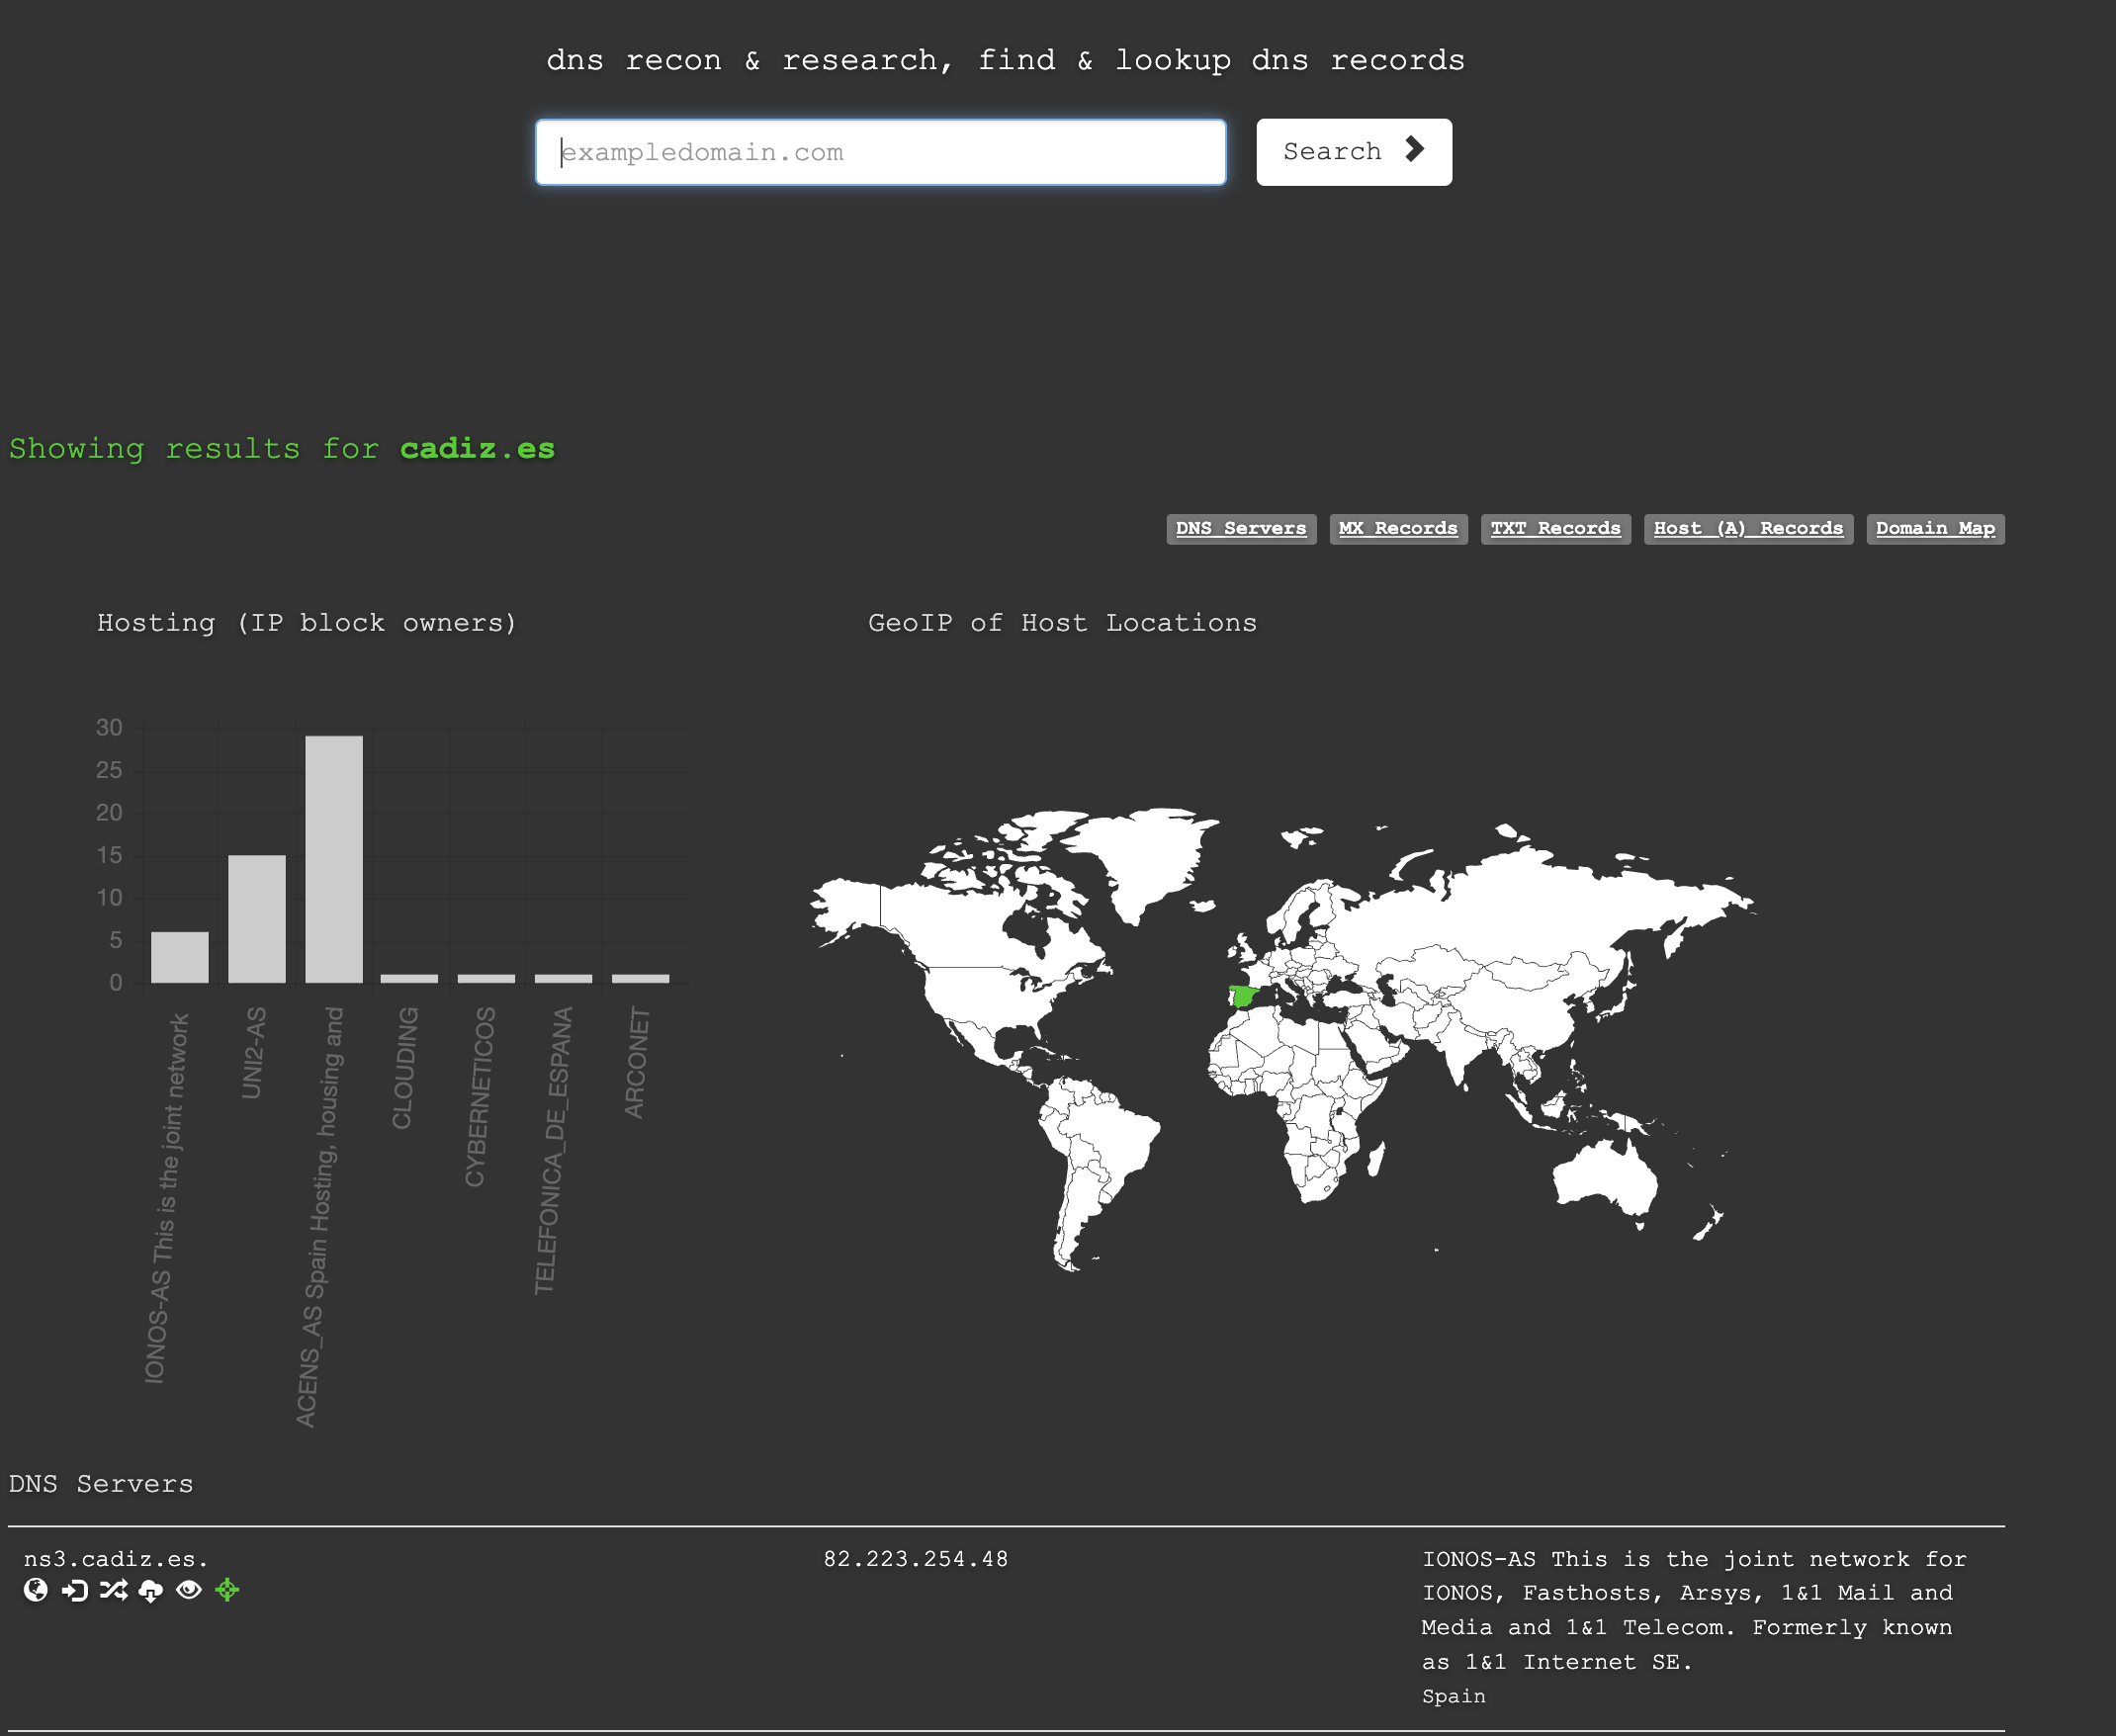
\includegraphics[width=.9\linewidth]{Practica 3y4/images/Screenshot 2024-10-31 at 09.06.31.png}
        \caption{Interfaz principal de DNSDumpster}
        \label{fig:enter-label}
    \end{minipage}
    \hfill
    \begin{minipage}{.5\textwidth}
        \centering
        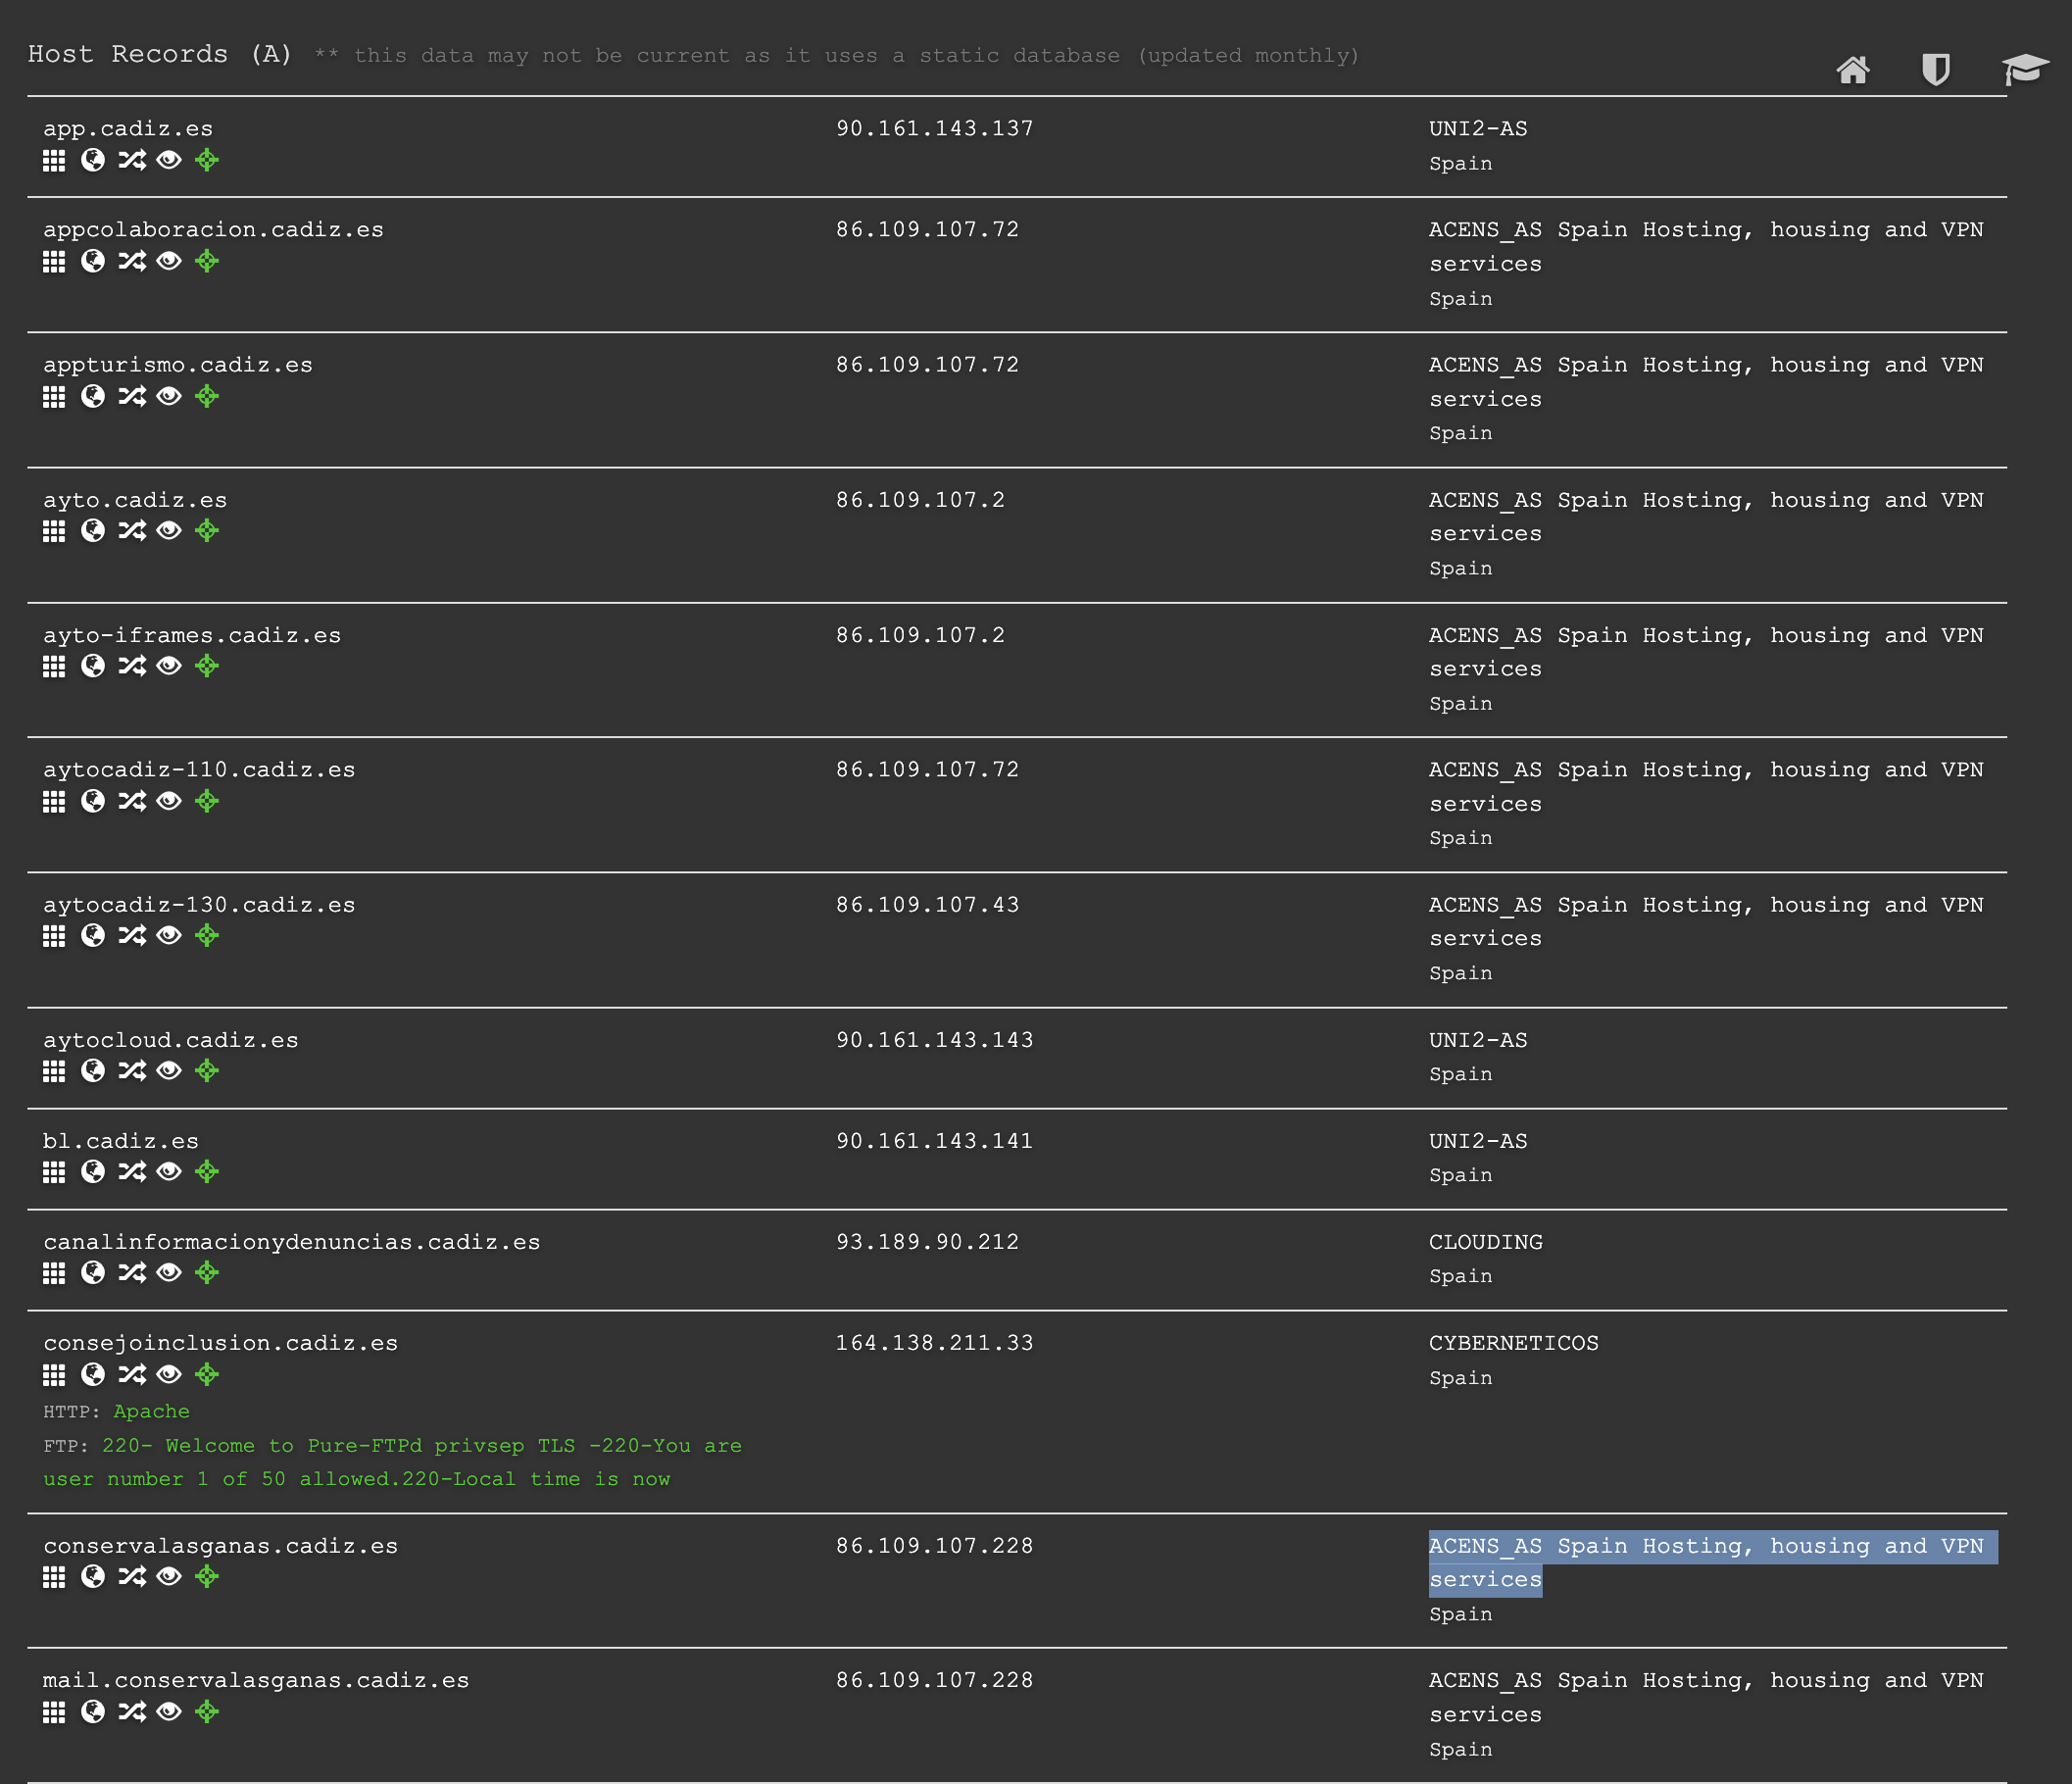
\includegraphics[width=.9\linewidth]{Practica 3y4/images/Screenshot 2024-10-31 at 09.13.01.png}
        \caption{Resultado de búsqueda de los subdominios cadiz.es}
        \label{fig:enter-label}
    \end{minipage}
    \end{figure}
    % \item \textit{¿Qué gestor de contenidos utilizan varios de los subdominios?}
    % \newline

    % \begin{figure}[h]
    %     \centering
    %     \includegraphics[width=0.5\linewidth]{}
    %     \caption{Caption}
    %     \label{fig:enter-label}
    % \end{figure}
        
    % \item \textit{¿Qué sistema operativo es el más probable que use el servidor que aloja el subdominio ftp.cadiz.es? ¿Por qué?}
    % \newline
    % Al ser hacer uso del servicio \textit{FTP} el Sistema Operativo más probable es una distrubución de Linux, en este caso:

    % \begin{figure}[h]
    %     \centering
    %     \includegraphics[width=0.5\linewidth]{}
    %     \caption{Caption}
    %     \label{fig:enter-label}
    % \end{figure}
    
\end{itemize}
\newpage
%%%%%%%%%%%%%%%%%%%%%%%%%%%%%%%%%%%%%%%%%%%%%%%%%%%%%%%%%%%%%%%%%%%%%%%%%%%%%%%%%%%%%%%%%
\section{Ejercicio 2}
\textit{Usando la herramienta DNS Trails~\cite{DNSTrail} liste los subdominios de diariodecadiz.es y responda a las siguientes preguntas:}
\begin{figure}[h]
    \centering
    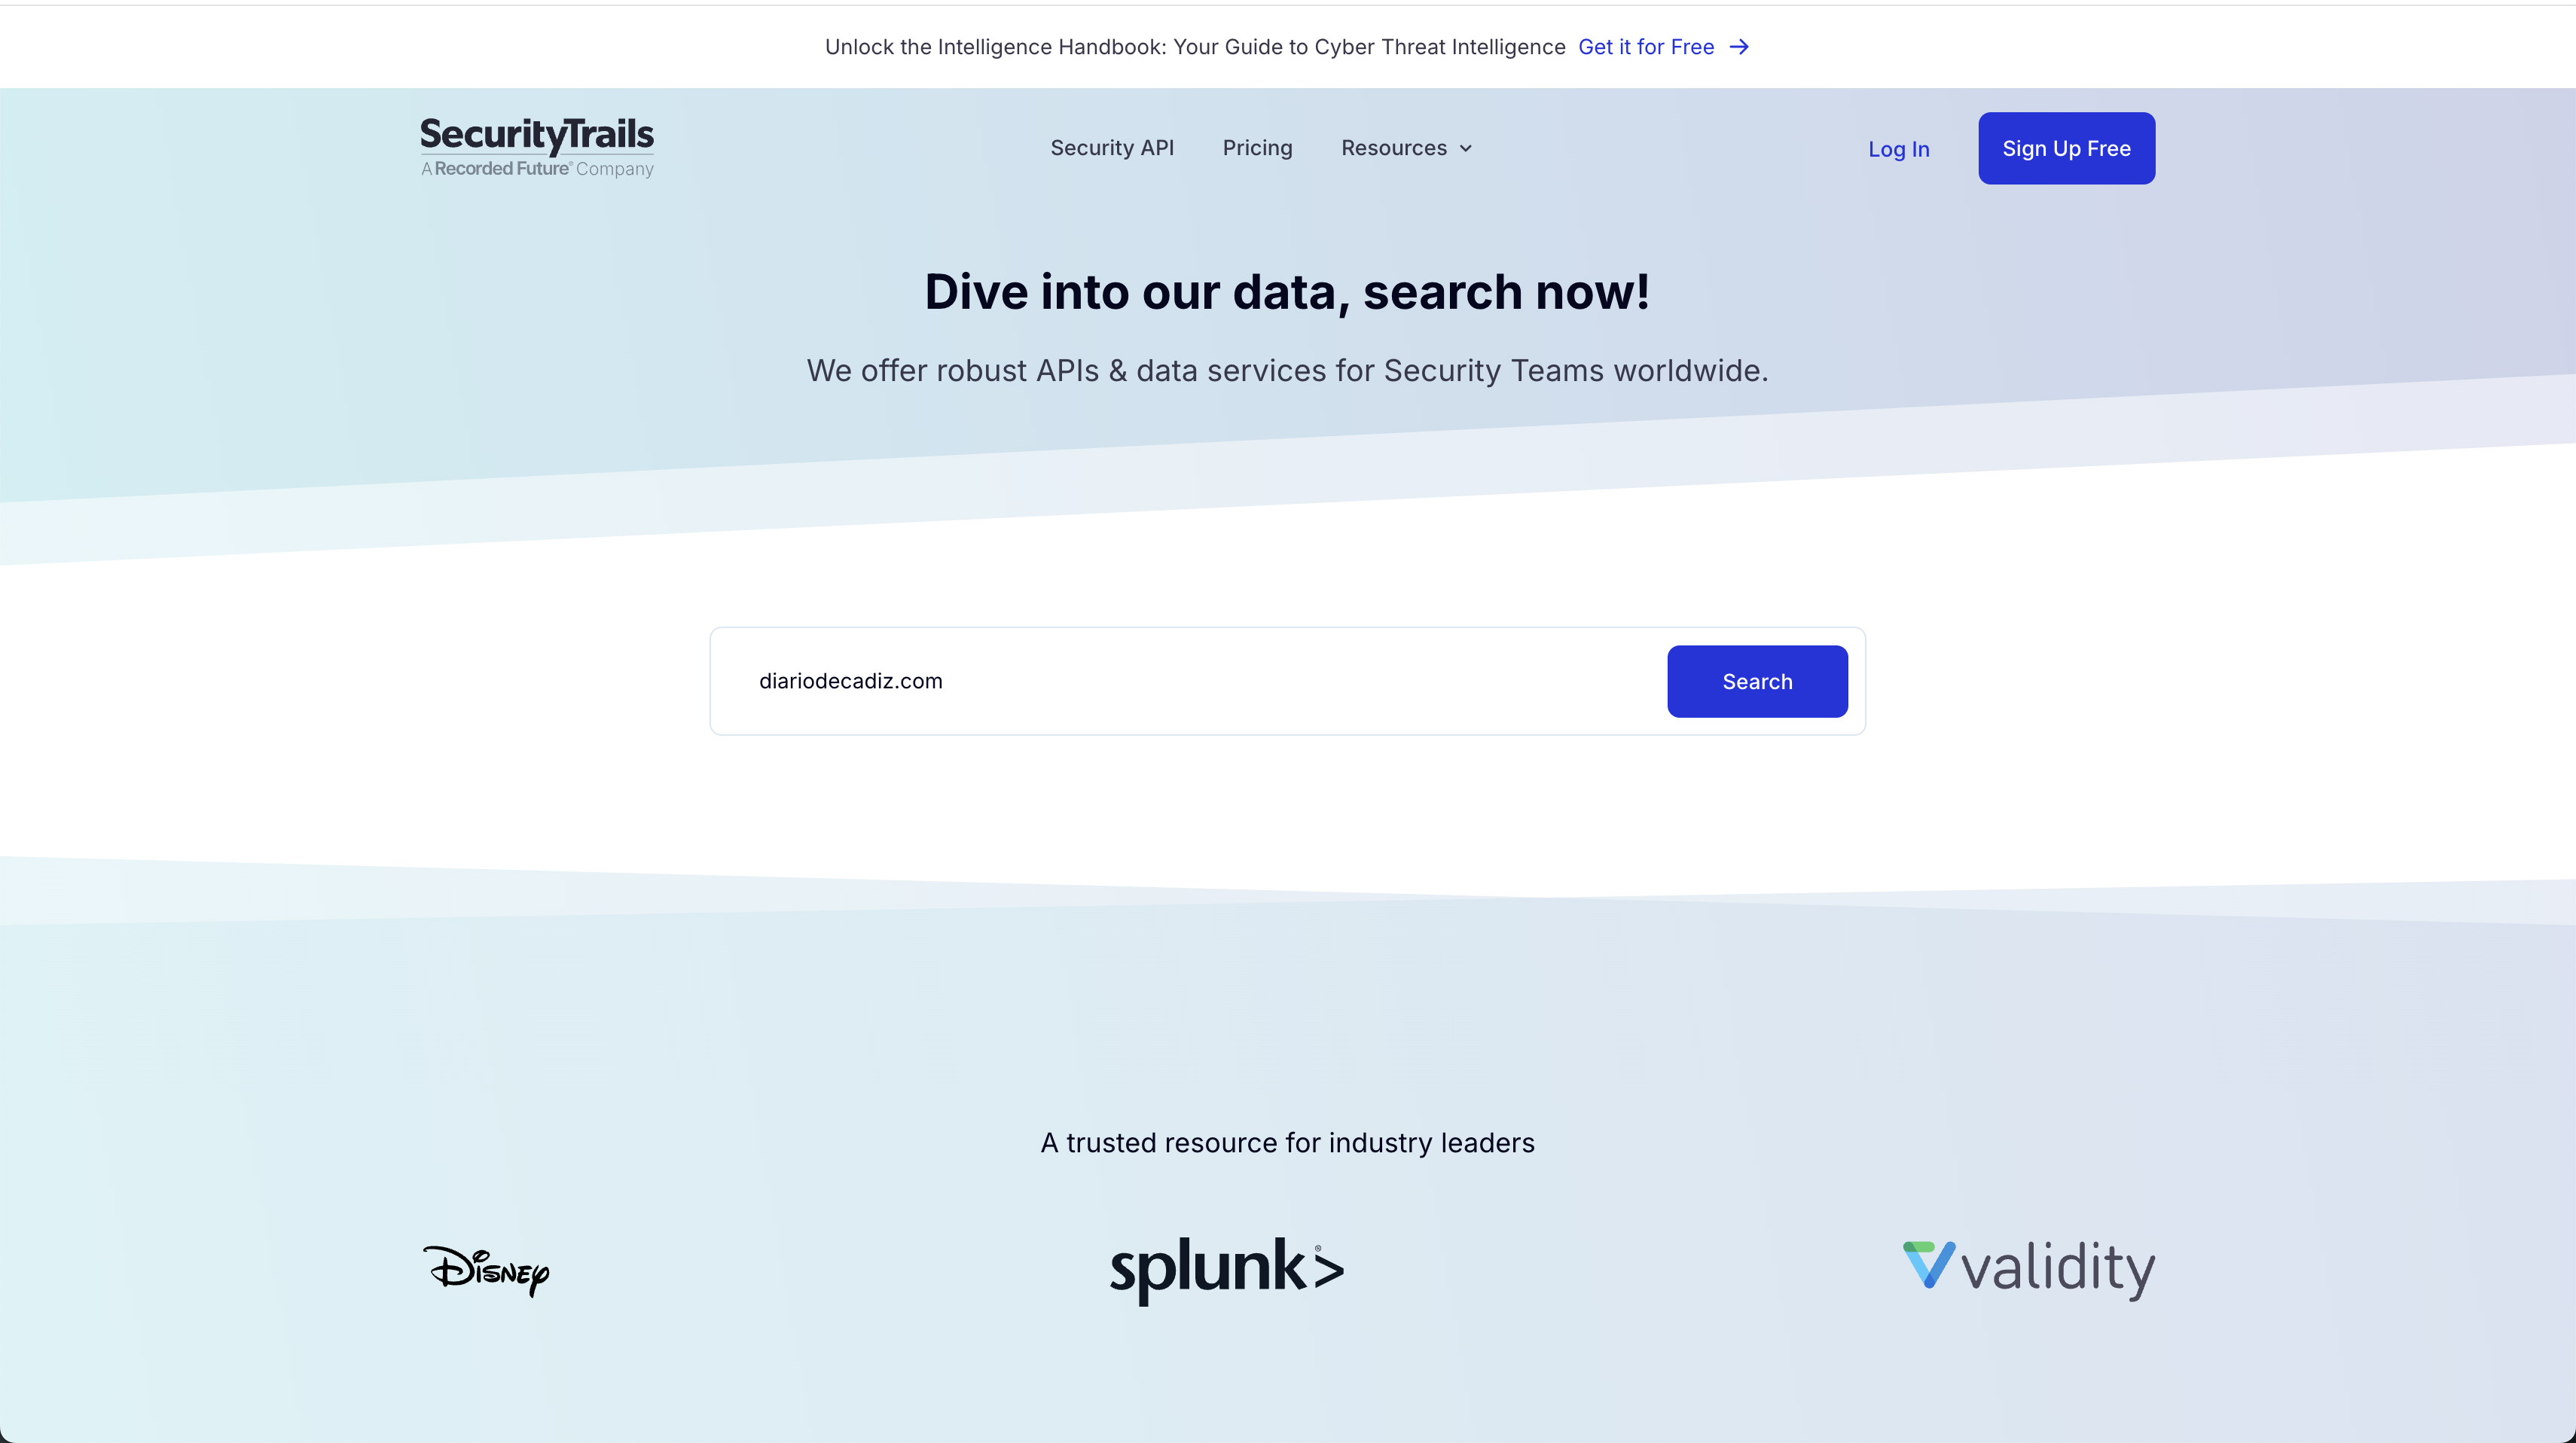
\includegraphics[width=\linewidth]{Practica 3y4/images/Screenshot 2024-10-31 at 09.41.49.png}
    \caption{Interfaz principal}
    \label{fig:enter-label}
\end{figure}
\begin{itemize}
    \item \textit{¿Cuántos subdominios encontramos?}
    \newline
    Encontramos 29 subdominios, como podemos ver en las figuras:
    \begin{figure}[h]
    \begin{minipage}{0.5\textwidth}
        \centering
        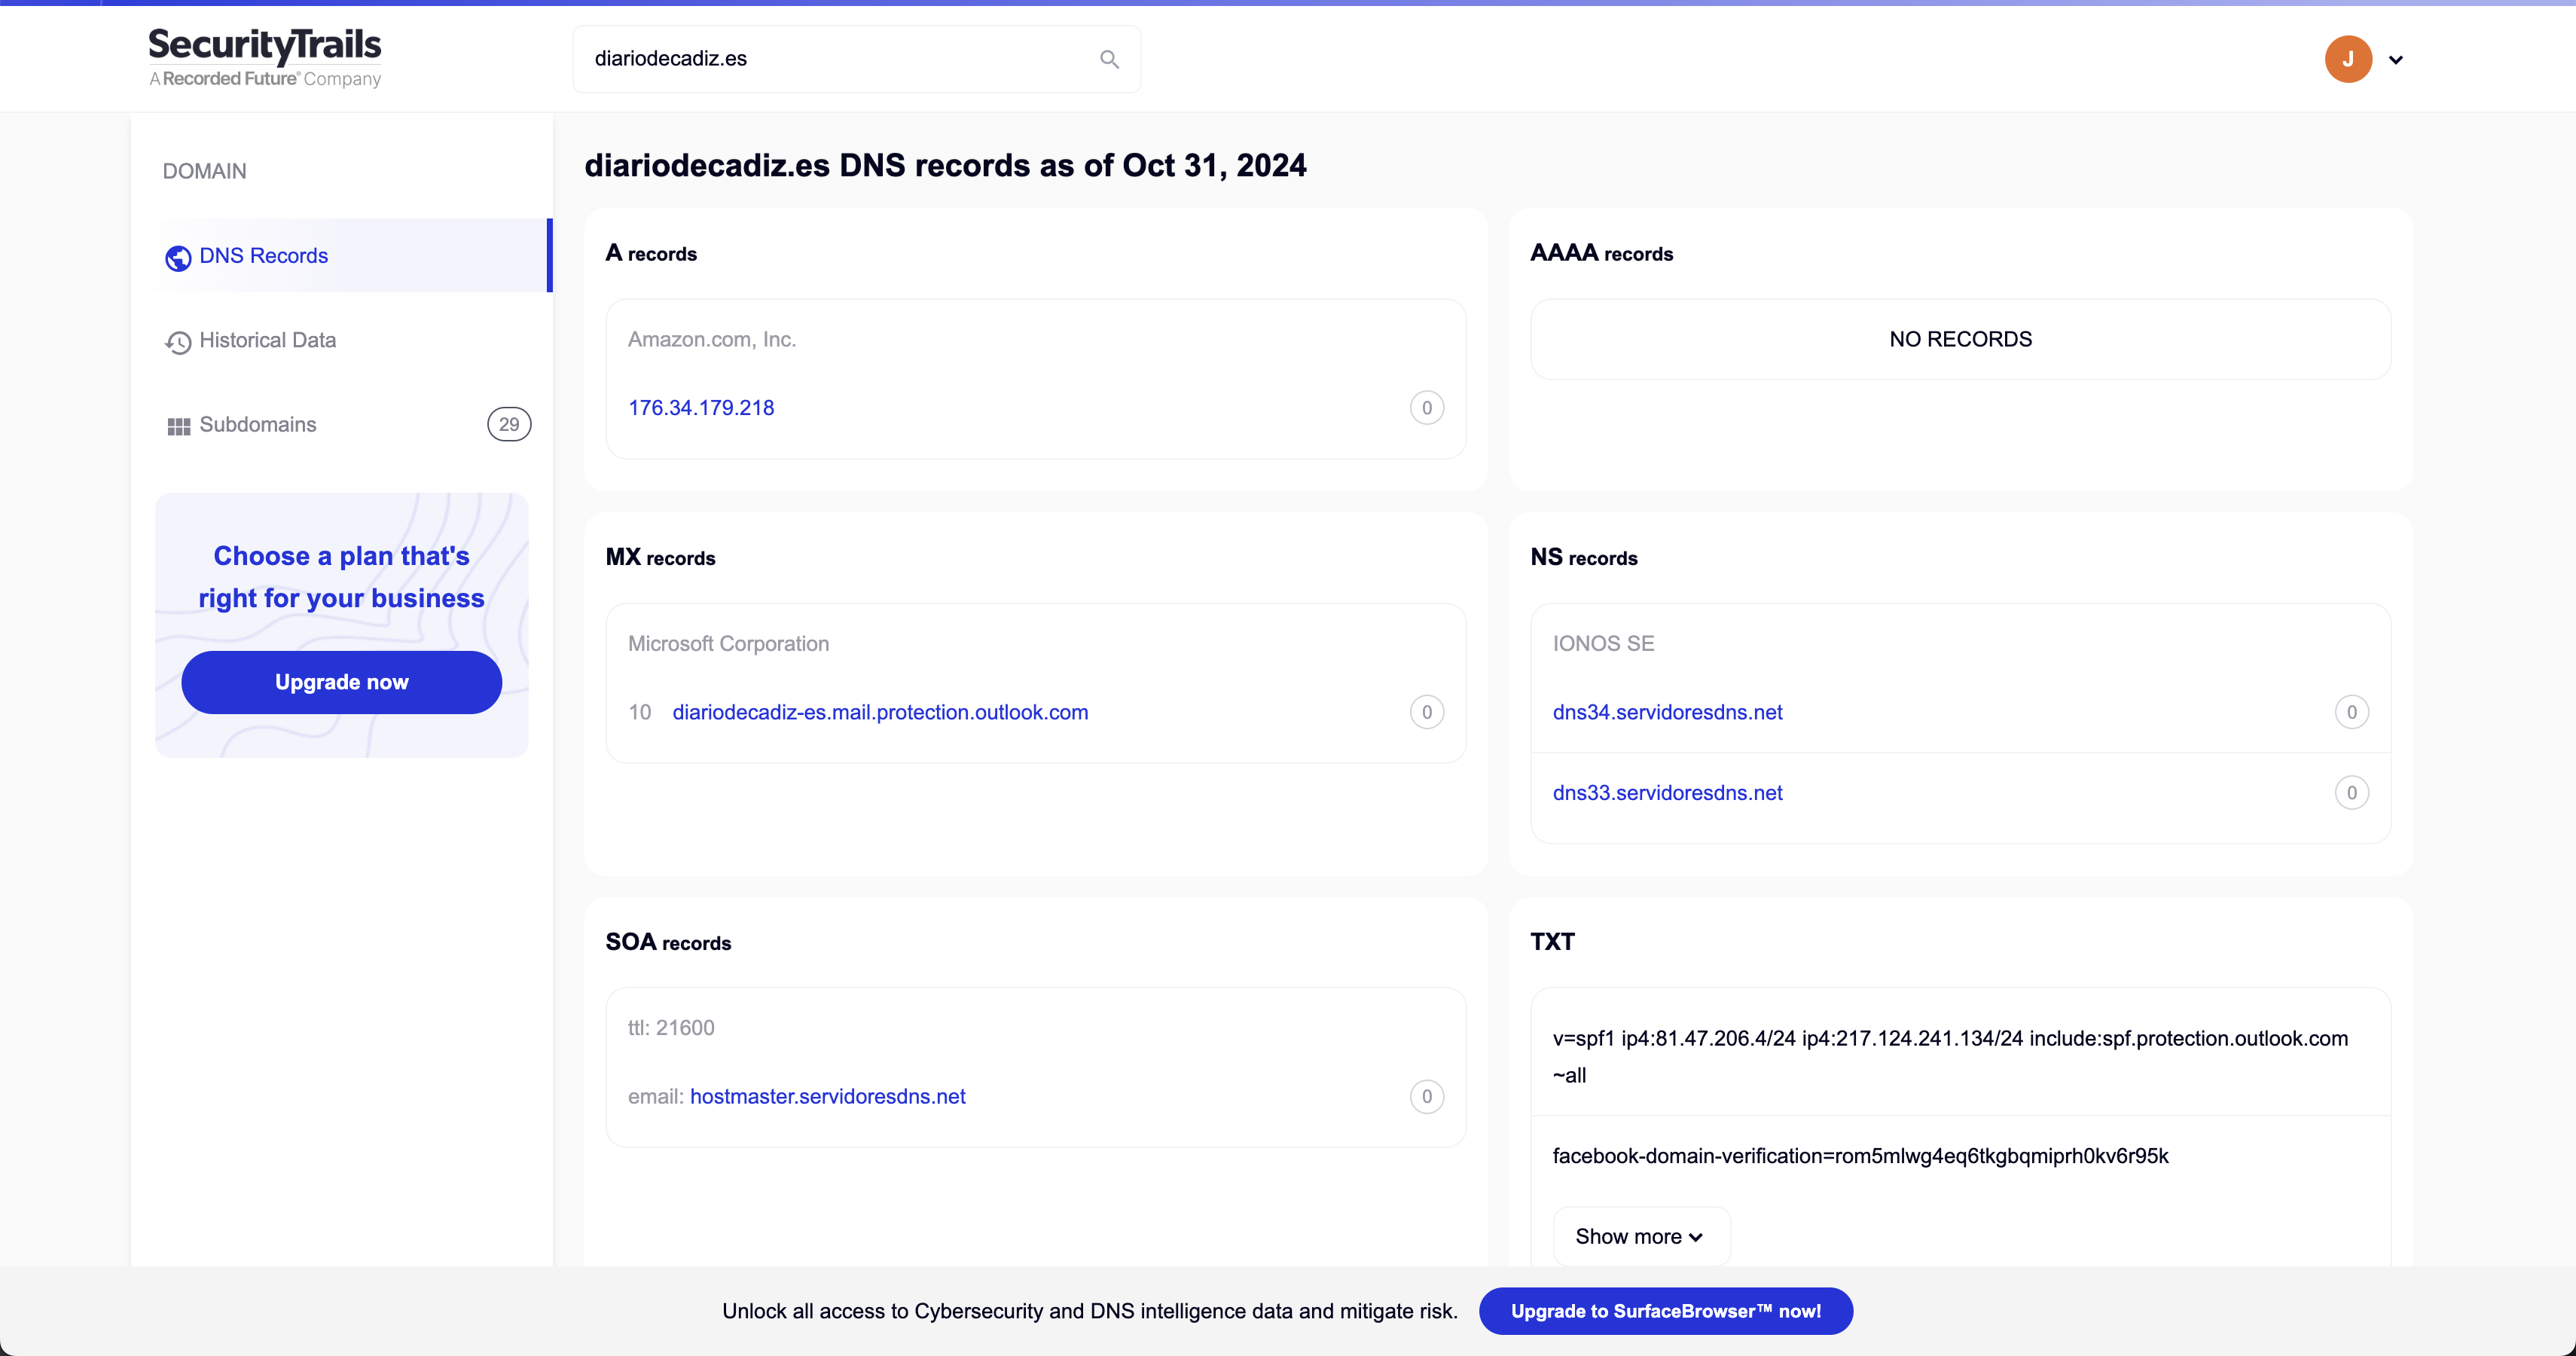
\includegraphics[width=.8\linewidth]{Practica 3y4/images/Screenshot 2024-10-31 at 09.50.15.png}
        \caption{Resultado de búsqueda del dominio.}
        \label{fig:enter-label}
    \end{minipage}
    \hfill
    \begin{minipage}{0.5\textwidth}
        \centering
        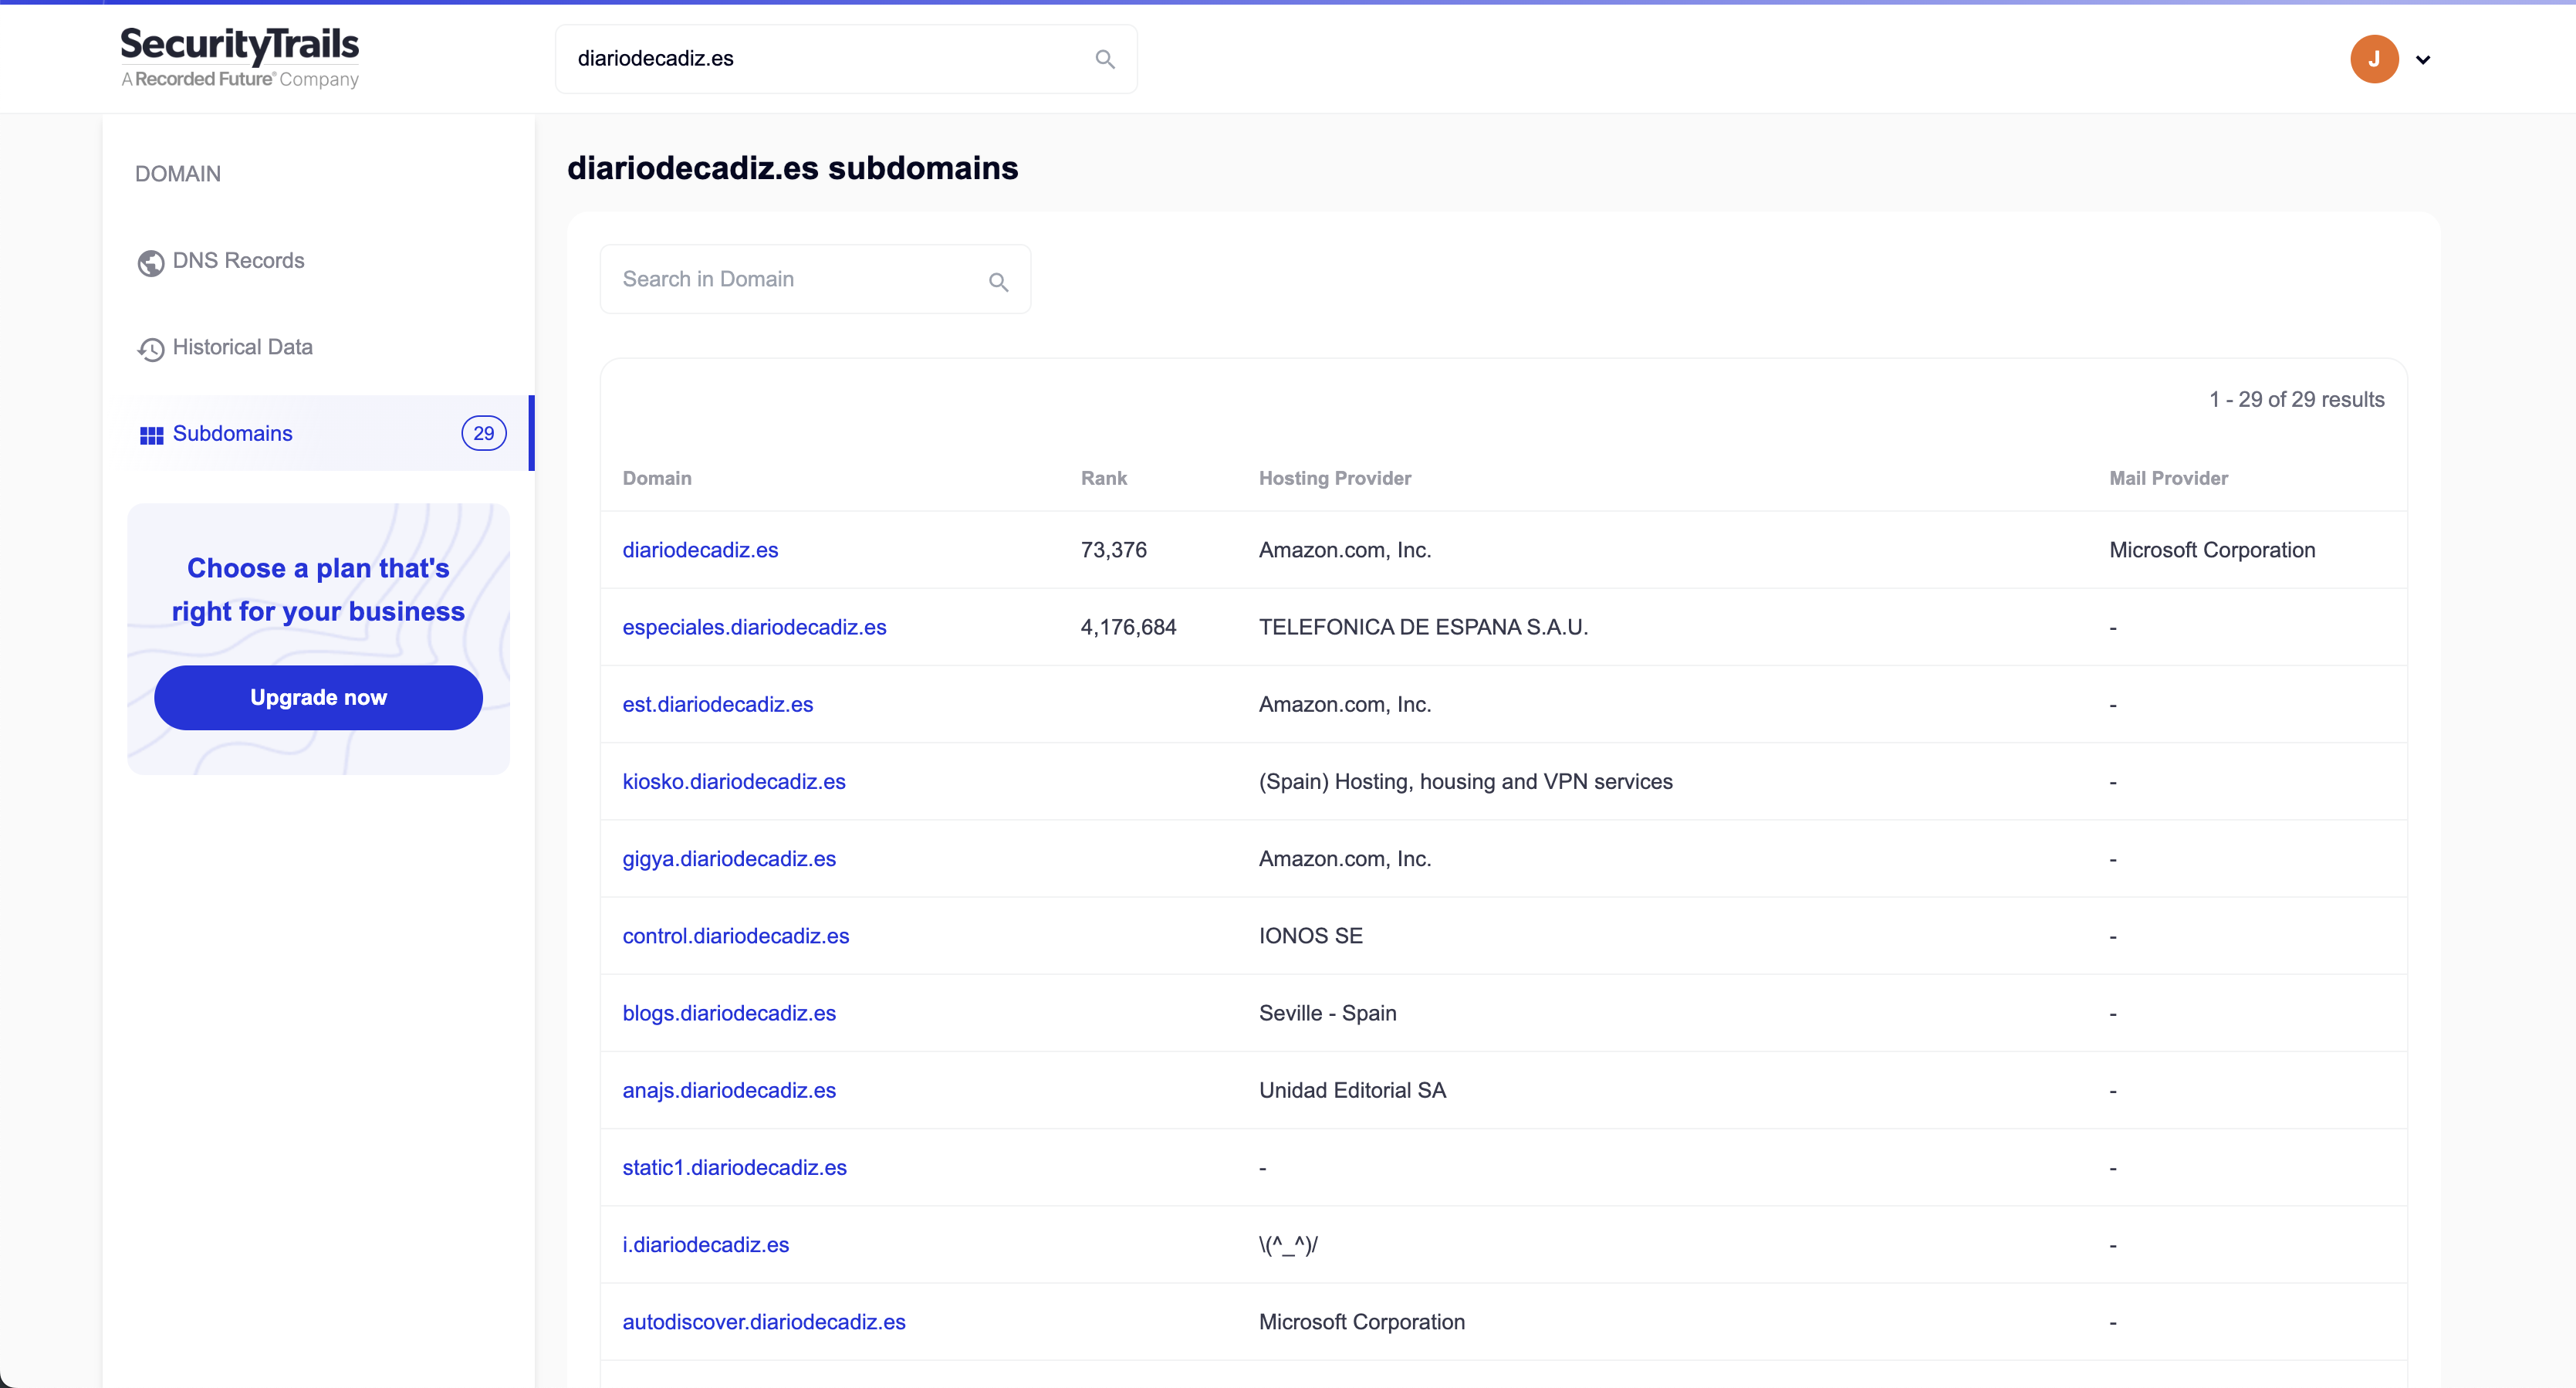
\includegraphics[width=.8\linewidth]{Practica 3y4/images/Screenshot 2024-10-31 at 09.51.30.png}
        \caption{Algunos subdominios}
        \label{fig:enter-label}
    \end{minipage}
    \end{figure}

    \item \textit{¿Quién provee el hosting a la página principal?}
    \newline
    Como podemos ver en la \textit{Figura 2.6}, el dominio de la página principal\\ \texttt{diariodecadiz.es} es \textbf{Amazon}.
    \newpage
    
    \item \textit{¿Qué subdominio es una redirección a un panel de login?}
    \newline
    Finalmente, en la \textit{Figura 2.8} podemos ver que el dominio\\ \texttt{https://panelcontrolhosting.com/} contiene lo siguiente:
    \begin{figure}[h]
        \centering
        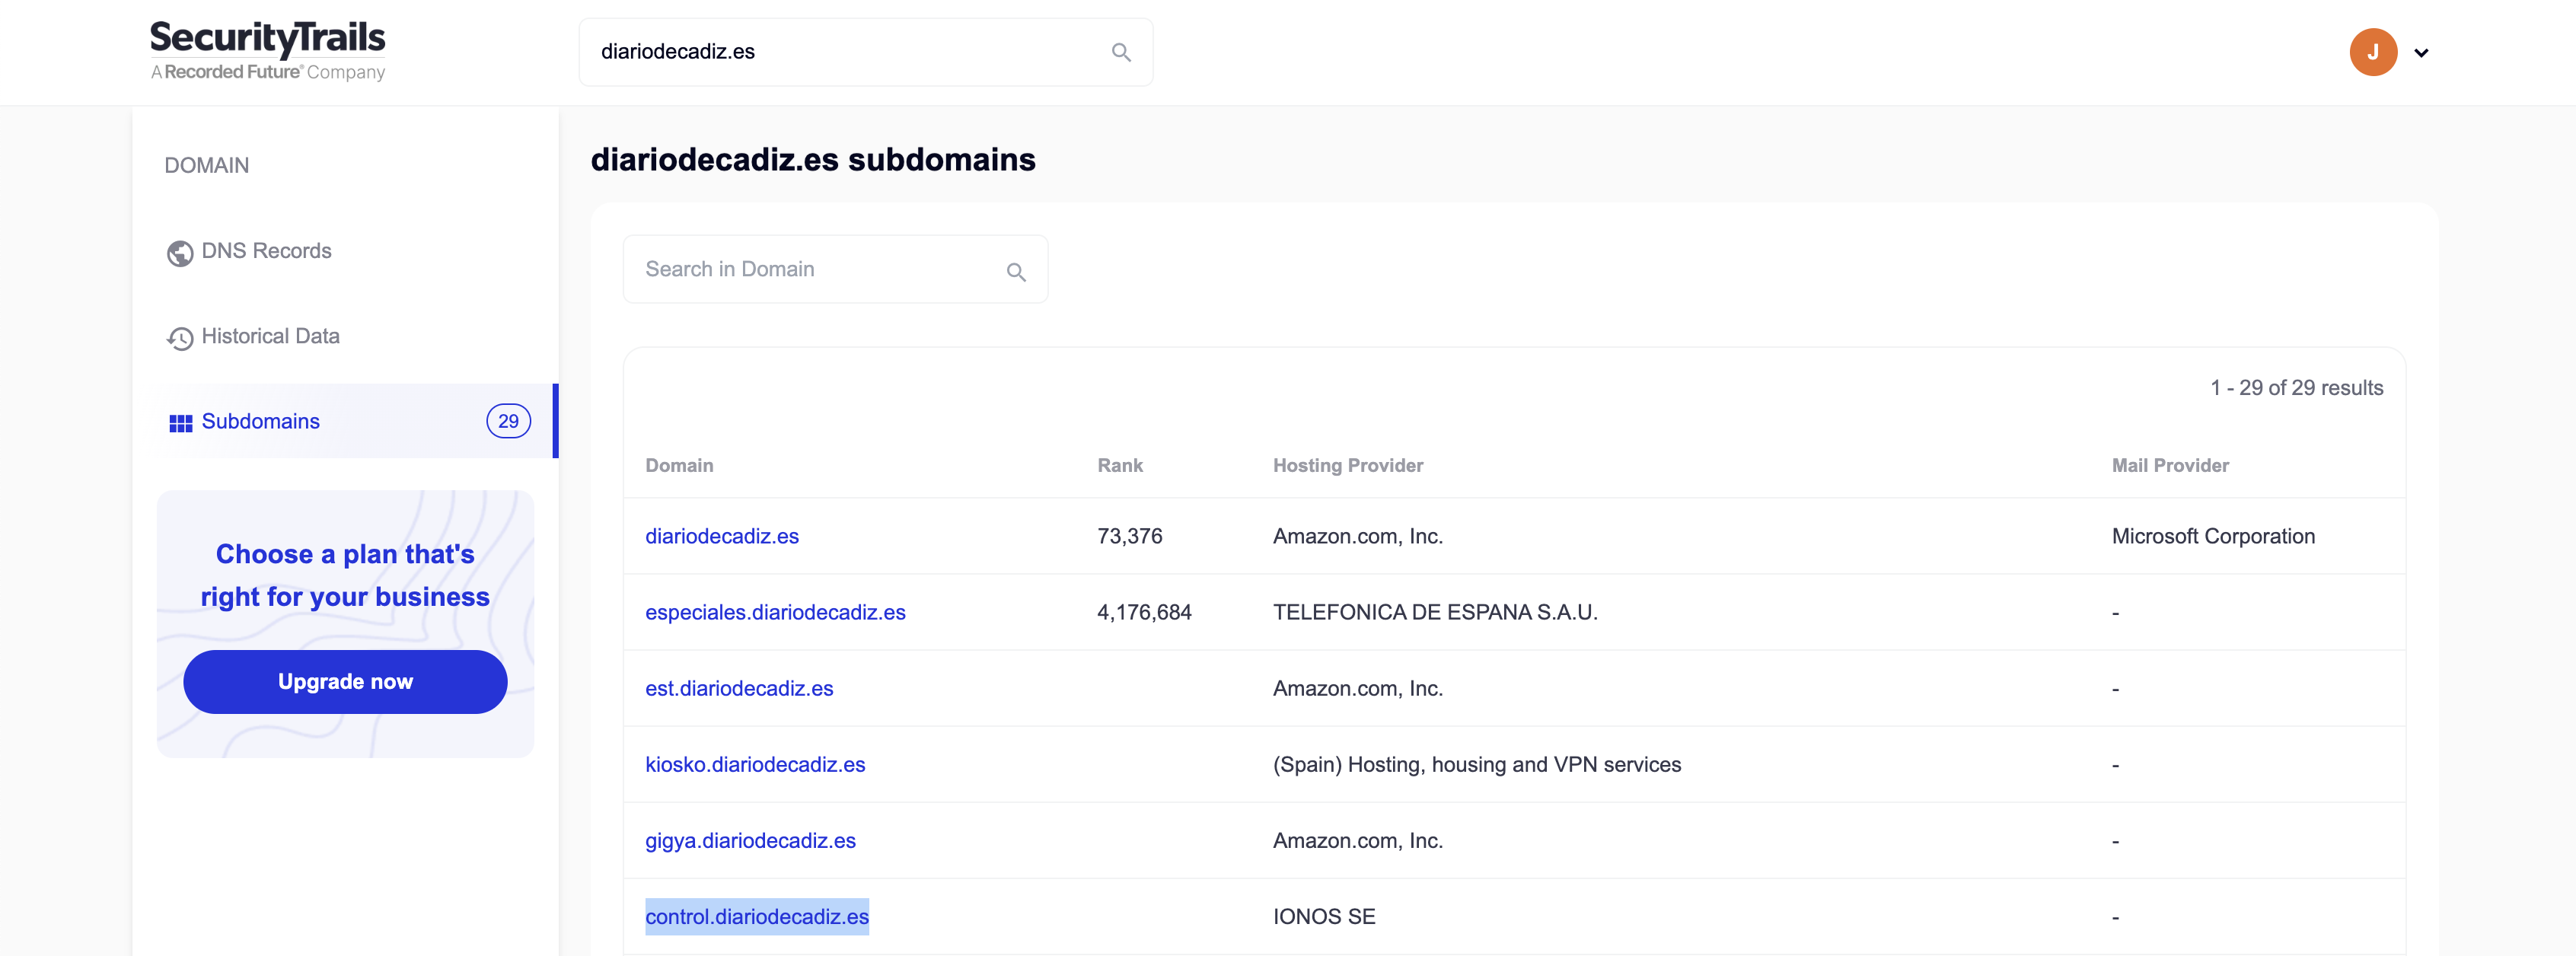
\includegraphics[width=.9\linewidth]{Practica 3y4/images/Screenshot 2024-10-31 at 09.56.50.png}
        \caption{Encontramos el subdominio del panel de login}
        \label{fig:enter-label}        
        \vspace{1cm}
        \centering
        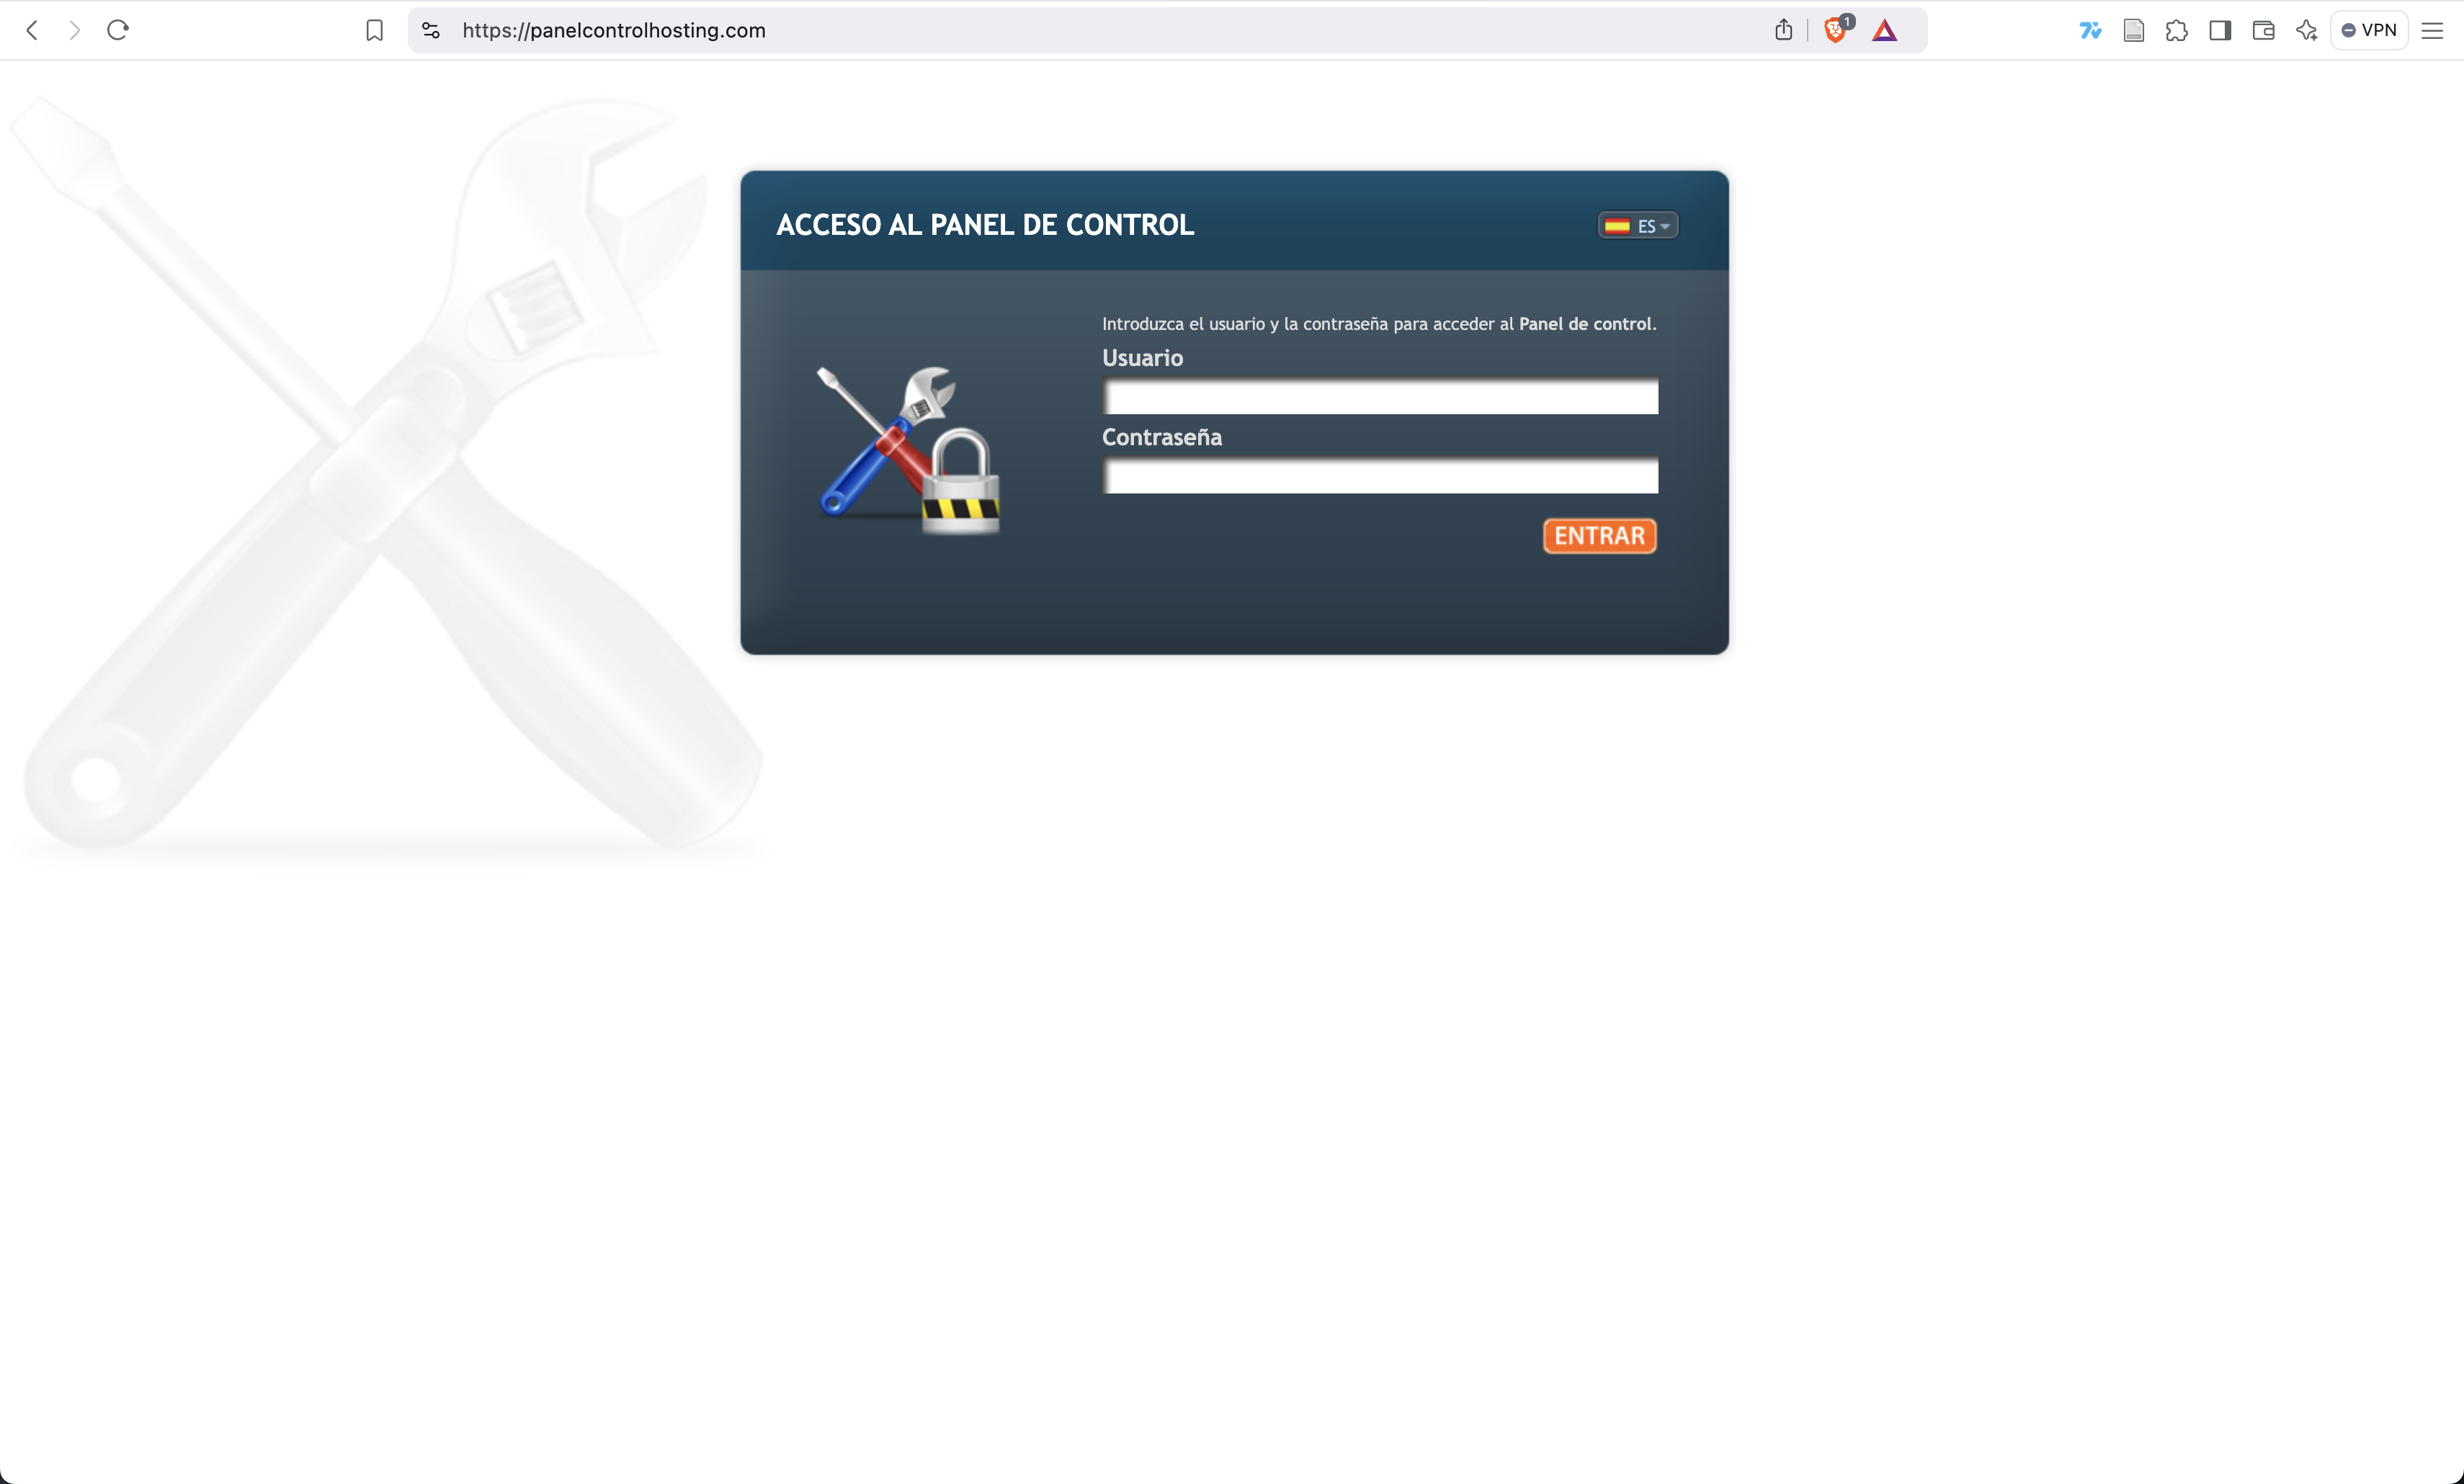
\includegraphics[width=.9\linewidth]{Practica 3y4/images/Screenshot 2024-10-31 at 09.57.02.png}
        \caption{Contenido del subdominio}
        \label{fig:enter-label}
    \end{figure}
\end{itemize}
\newpage
%%%%%%%%%%%%%%%%%%%%%%%%%%%%%%%%%%%%%%%%%%%%%%%%%%%%%%%%%%%%%%%%%%%%%%%%%%%%%%%%%%%%%%%%%
\section{Ejercicio 3}
\textit{Haciendo uso de Whois Lookup, conteste a las siguientes preguntas:}
\begin{itemize}
    \item \textit{¿Qué información podemos obtener sobre el dominio cadizturismo.com?}\\
        \begin{figure}[h]
            \centering
            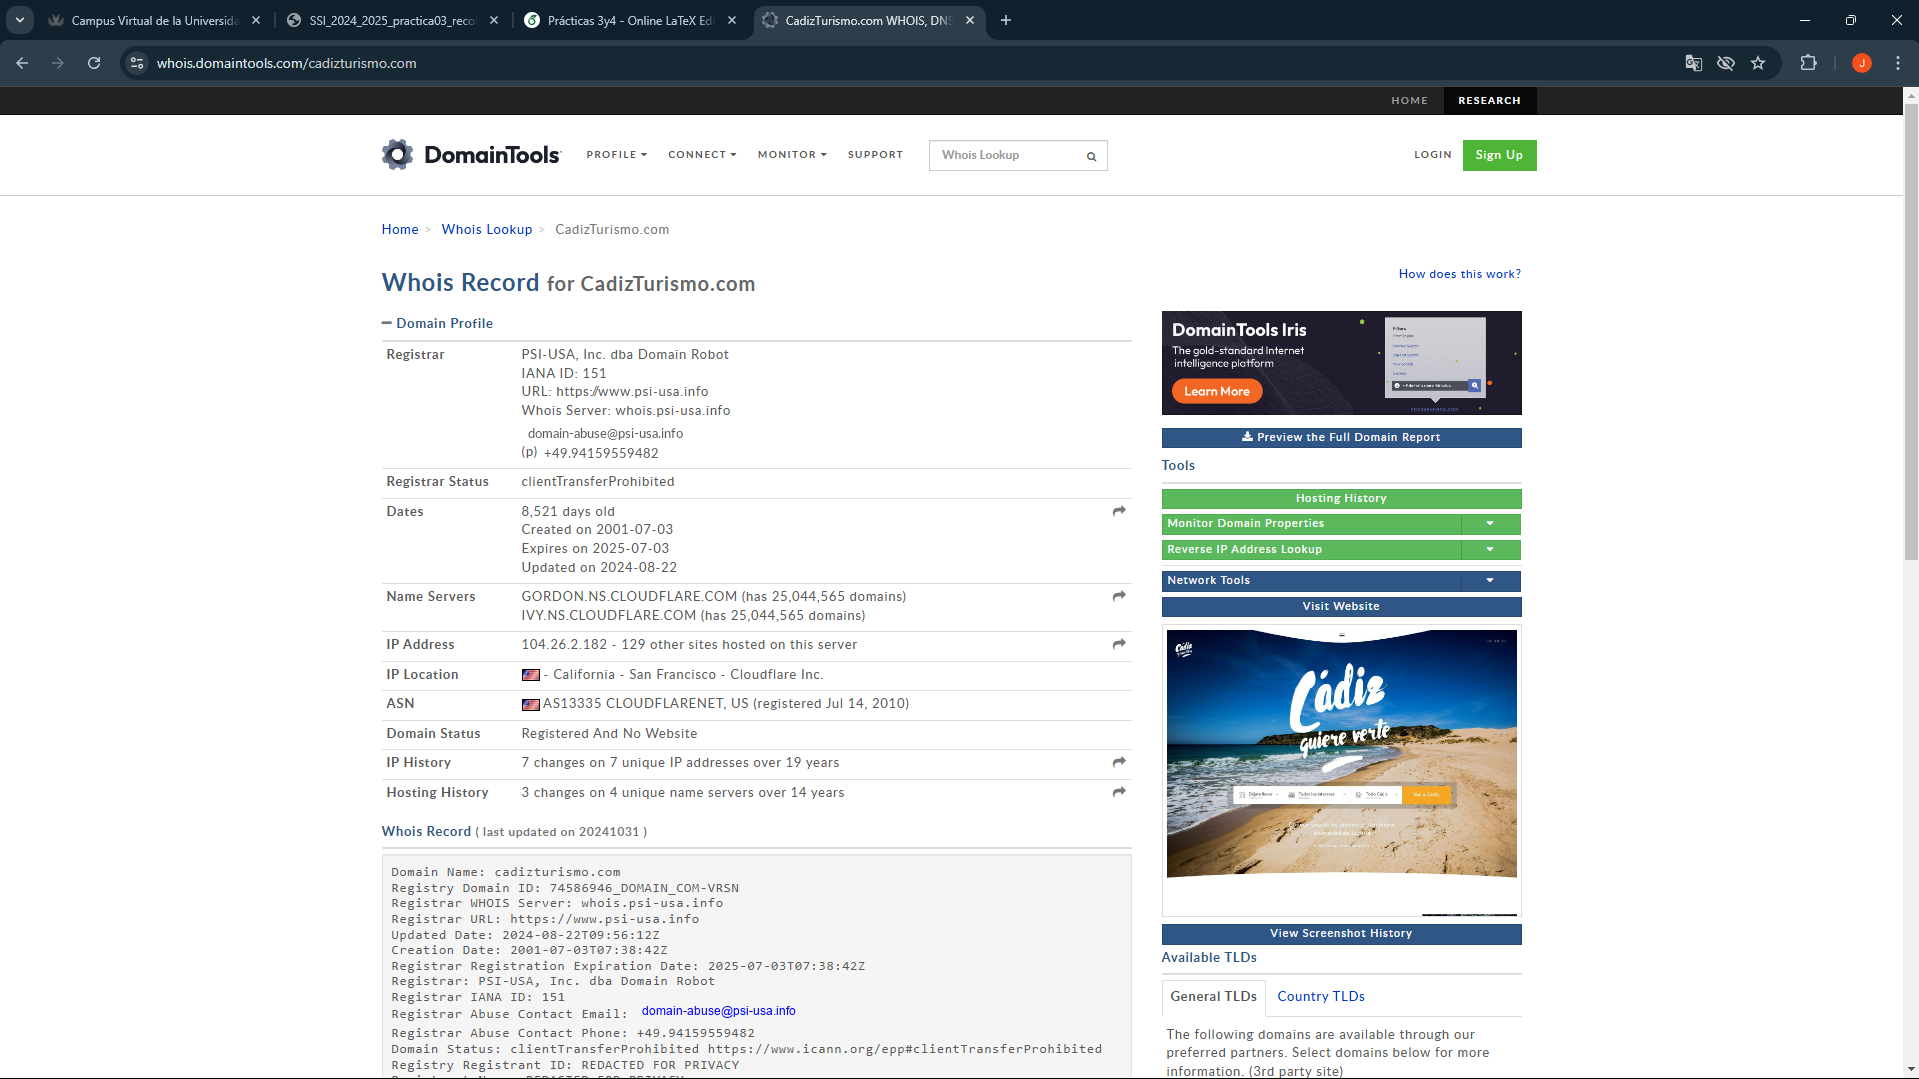
\includegraphics[width=0.5\linewidth]{Practica 3y4/images/cadizturismo.png}
            \caption{Uso de Whois Lookup para cadizturismo.com}
            \label{fig:enter-label}
        \end{figure}
        \\
        Podemos obrtener bastante información como; la ip, el id de IANA, la ubicación, los cambios (hosting), etc.
    \item \textit{¿Quién es el registrador de cadiz.com?}\\
        \begin{figure}[h]
            \centering
            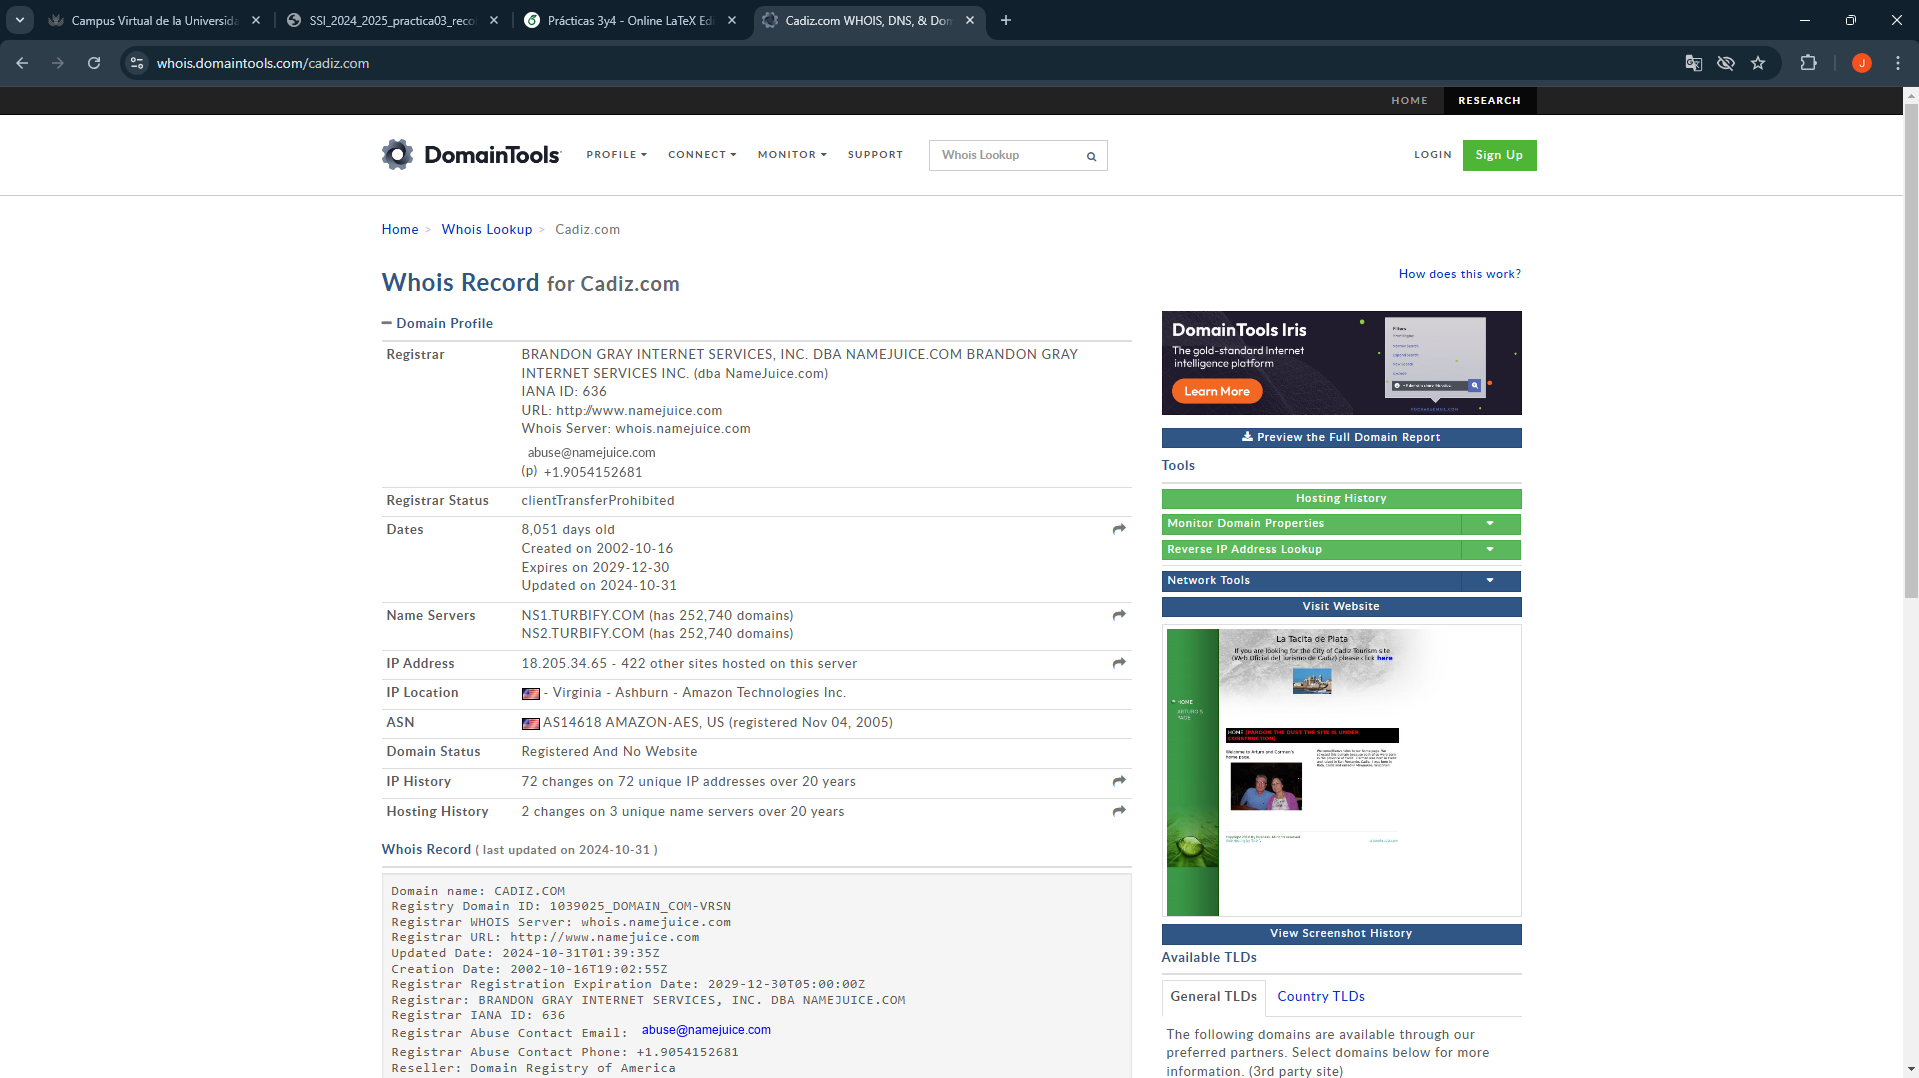
\includegraphics[width=0.5\linewidth]{Practica 3y4/images/cadiz.png}
            \caption{Uso de Whois Lookup para cadiz.com}
            \label{fig:enter-label}
        \end{figure}
        \\
        El registrador es \textit{BRANDON GRAY INTERNET SERVICES}, que operaba como \textit{NameJuice.com}, era un operador de registro de nombres de dominio acreditado por ICANN con sede en Markham, Ontario.
\end{itemize}
\newpage
%%%%%%%%%%%%%%%%%%%%%%%%%%%%%%%%%%%%%%%%%%%%%%%%%%%%%%%%%%%%%%%%%%%%%%%%%%%%%%%%%%%%%%%%%
\section{Ejercicio 4}
\textit{Haciendo uso de la información encontrada a través de la extensión Wappalyzer,
conteste a las siguientes preguntas:}\\

    \begin{figure}[h]
        \centering
        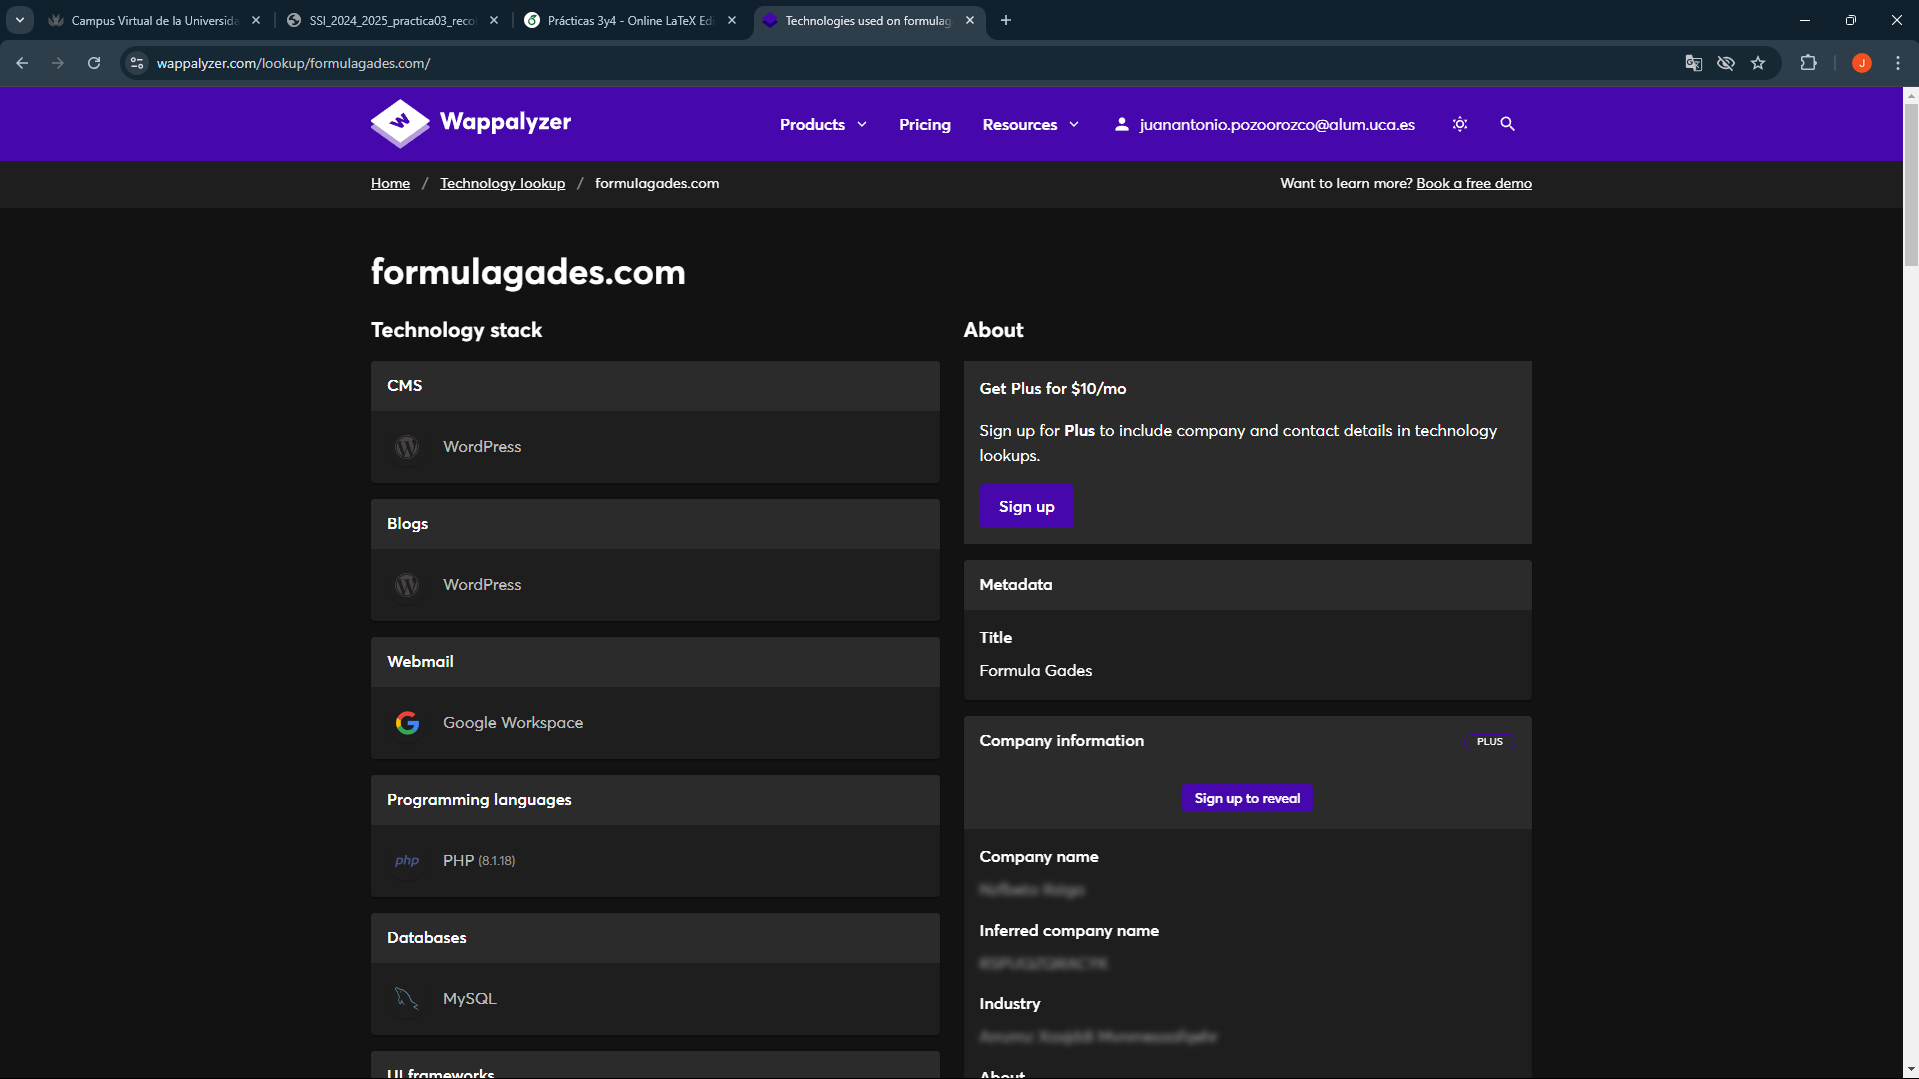
\includegraphics[width=0.5\linewidth]{Practica 3y4/images/Captura de pantalla 2024-10-31 112257.png}
        \caption{Ejemplo de uso de Wappalyzer}
        \label{fig:enter-label}
    \end{figure}
    
    \begin{itemize}
        \item \textit{¿Qué versión de Apache se usa en directorio.uca.es?}\\
            La dirección dada usa \textit{Apache Tomacat} y \textit{Apache HTTP Server 2.4.37}.
        \item \textit{¿Qué versión de PHP se usa en formulagades.com?}\\
            Usa la versión de PHP 8.1.18.
        \item \textit{¿Qué proxy está usando https://esingenieria.uca.es/?}\\
            Está usando Nginx.
    \end{itemize}
\newpage
%%%%%%%%%%%%%%%%%%%%%%%%%%%%%%%%%%%%%%%%%%%%%%%%%%%%%%%%%%%%%%%%%%%%%%%%%%%%%%%%%%%%%%%%%
\section{Ejercicio 5}
\textit{}
\begin{itemize}
    \item 
\end{itemize}
\newpage
%%%%%%%%%%%%%%%%%%%%%%%%%%%%%%%%%%%%%%%%%%%%%%%%%%%%%%%%%%%%%%%%%%%%%%%%%%%%%%%%%%%%%%%%%
\section{Ejercicio 6}
\textit{}
\begin{itemize}
    \item 
\end{itemize}
\newpage
%%%%%%%%%%%%%%%%%%%%%%%%%%%%%%%%%%%%%%%%%%%%%%%%%%%%%%%%%%%%%%%%%%%%%%%%%%%%%%%%%%%%%%%%%
\section{Ejercicio 7}
\textit{}
\begin{itemize}
    \item 
\end{itemize}

%%%%%%%%%%%%%%%%%%%%%%%%%%%%%%%%%%%%%%%%%%%%%%%%%%%%%%%%
\chapter{Práctica 4: Escaneo y enumeración de activos}

%%%%%%%%%%%%%%%%%%%%%%%%%%%%%%%%%%%%%%%%%%%%%%%%%%%%%%%%
\section{Ejercicio 1}
\textit{Ejecute la siguiente orden: \texttt{tcpping www.diariodecadiz.com}}
\begin{itemize}
    \item \textit{Describa la salida que ha obtenido.}
    \begin{figure}[h]
        \centering
        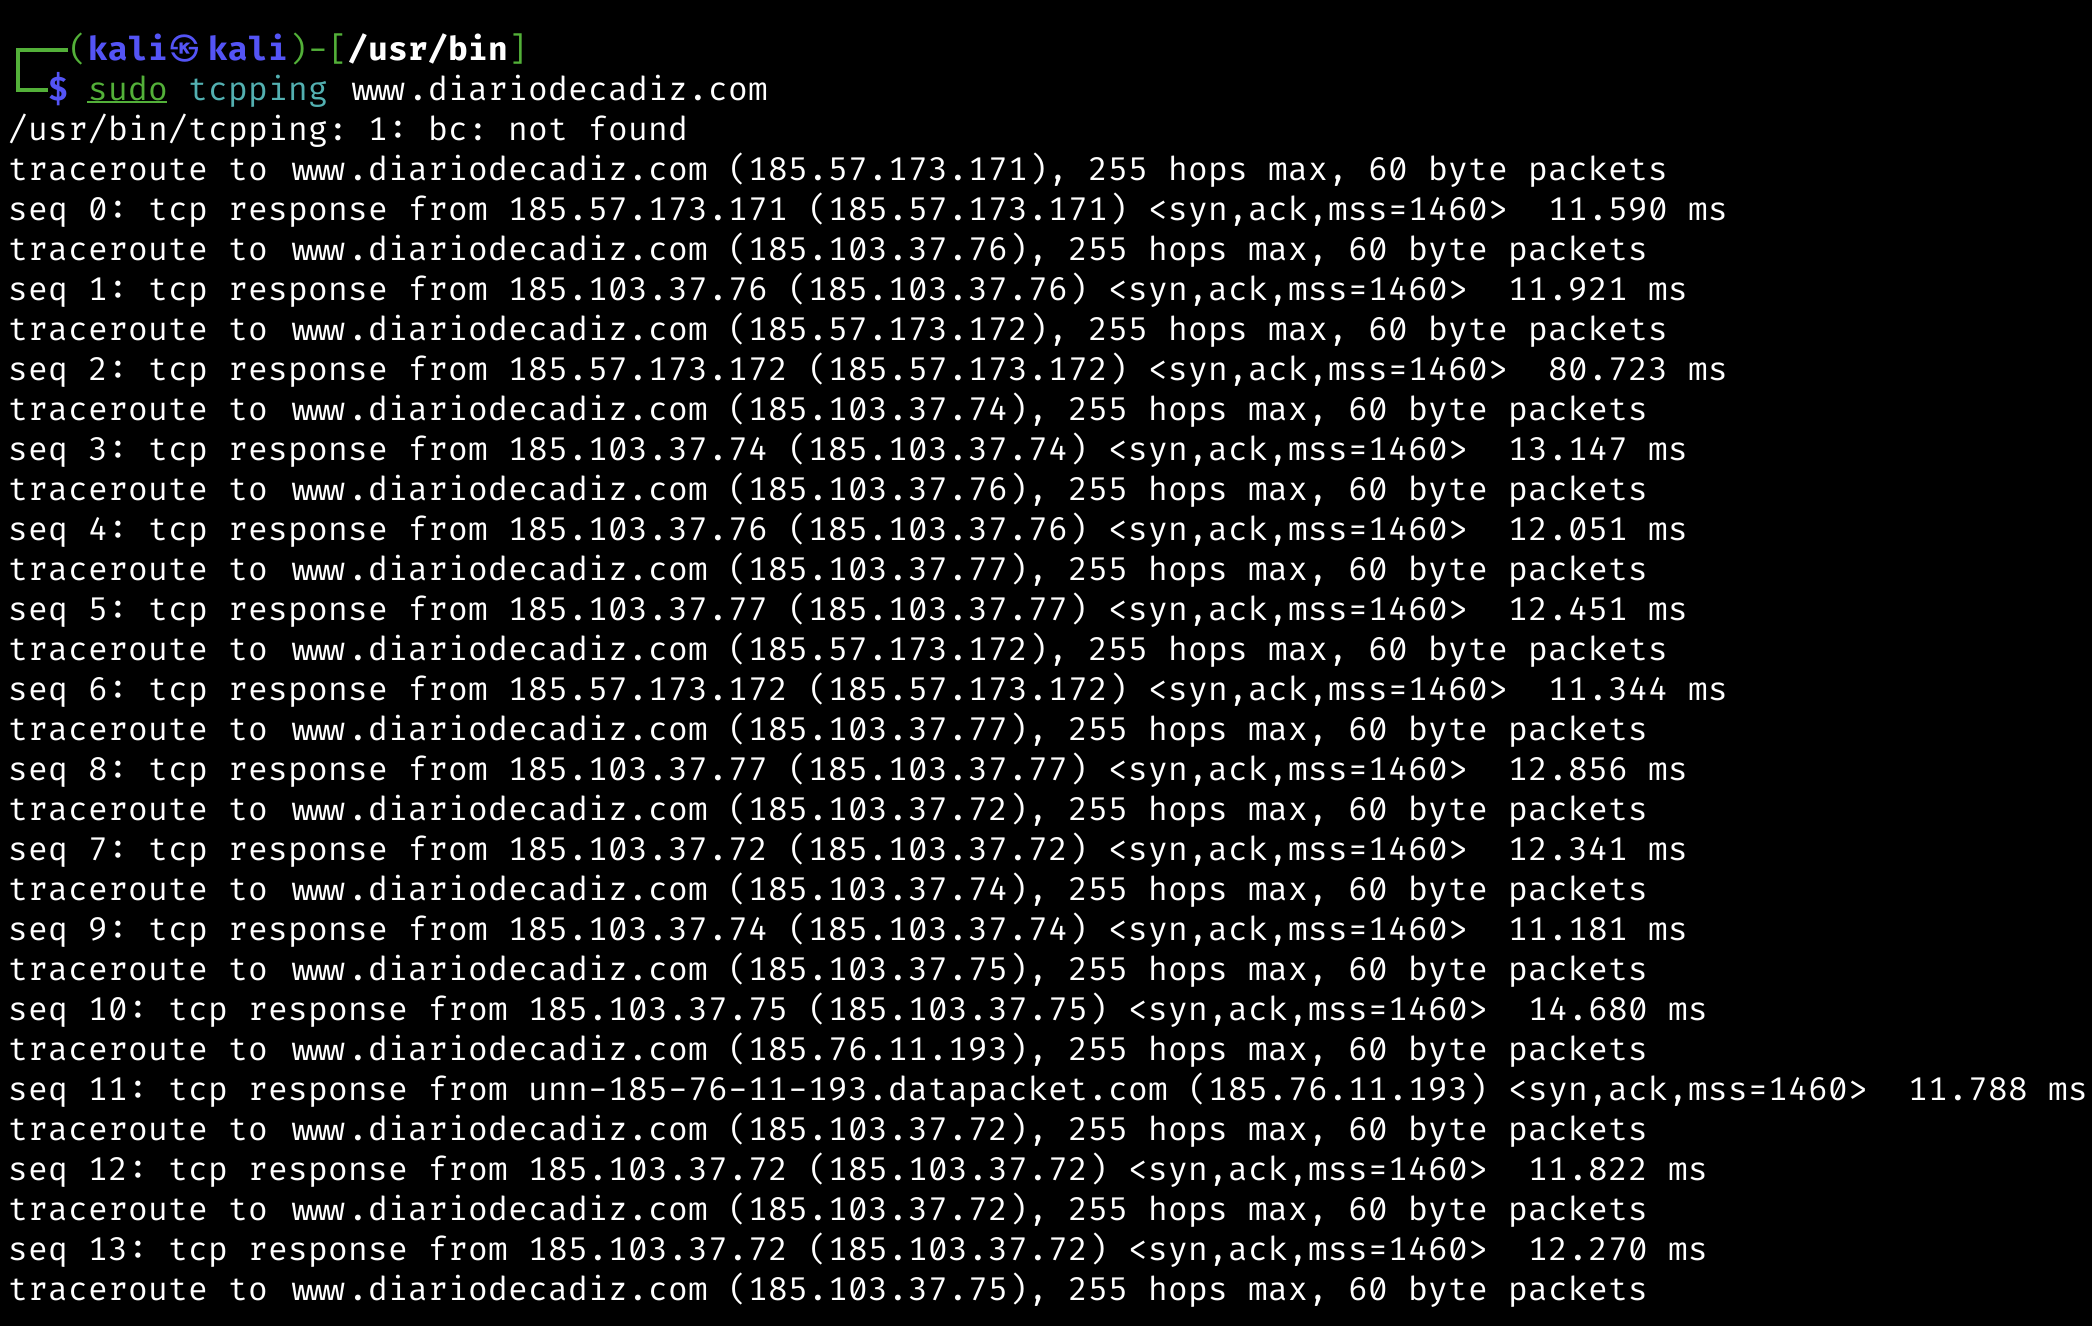
\includegraphics[width=.7\linewidth]{Practica 3y4/images/Screenshot 2024-11-07 at 20.09.25.png}
        \caption{Uso con una página web}
        \label{fig:enter-label}
    \end{figure}
    \item \textit{¿En qué se diferencia de un ping tradicional?}
    \newline
    \newline
    Vemos que tcpping realiza conexiones TCP mientras que ping hace uso del protocolo ICMP.
\end{itemize}
\textit{Ahora seleccione una dirección IP de su red local, puede ser un ordenador portátil,
un teléfono móvil, o cualquier otro que tenga a mano.}

\begin{itemize}
    \item \textit{¿Qué ocurre si hacemos tcpping a esa dirección? Justifique su respuesta.}
    \newline
    \newline
    Vemos que al ser un dispositivo que está en loca y no una página web la latencia es mucho menor así como el alcance de red, además vemos que los firewalls de los dispositivos locales no son tan restrictivos que los de una web.
    \begin{figure}[h]
        \centering
        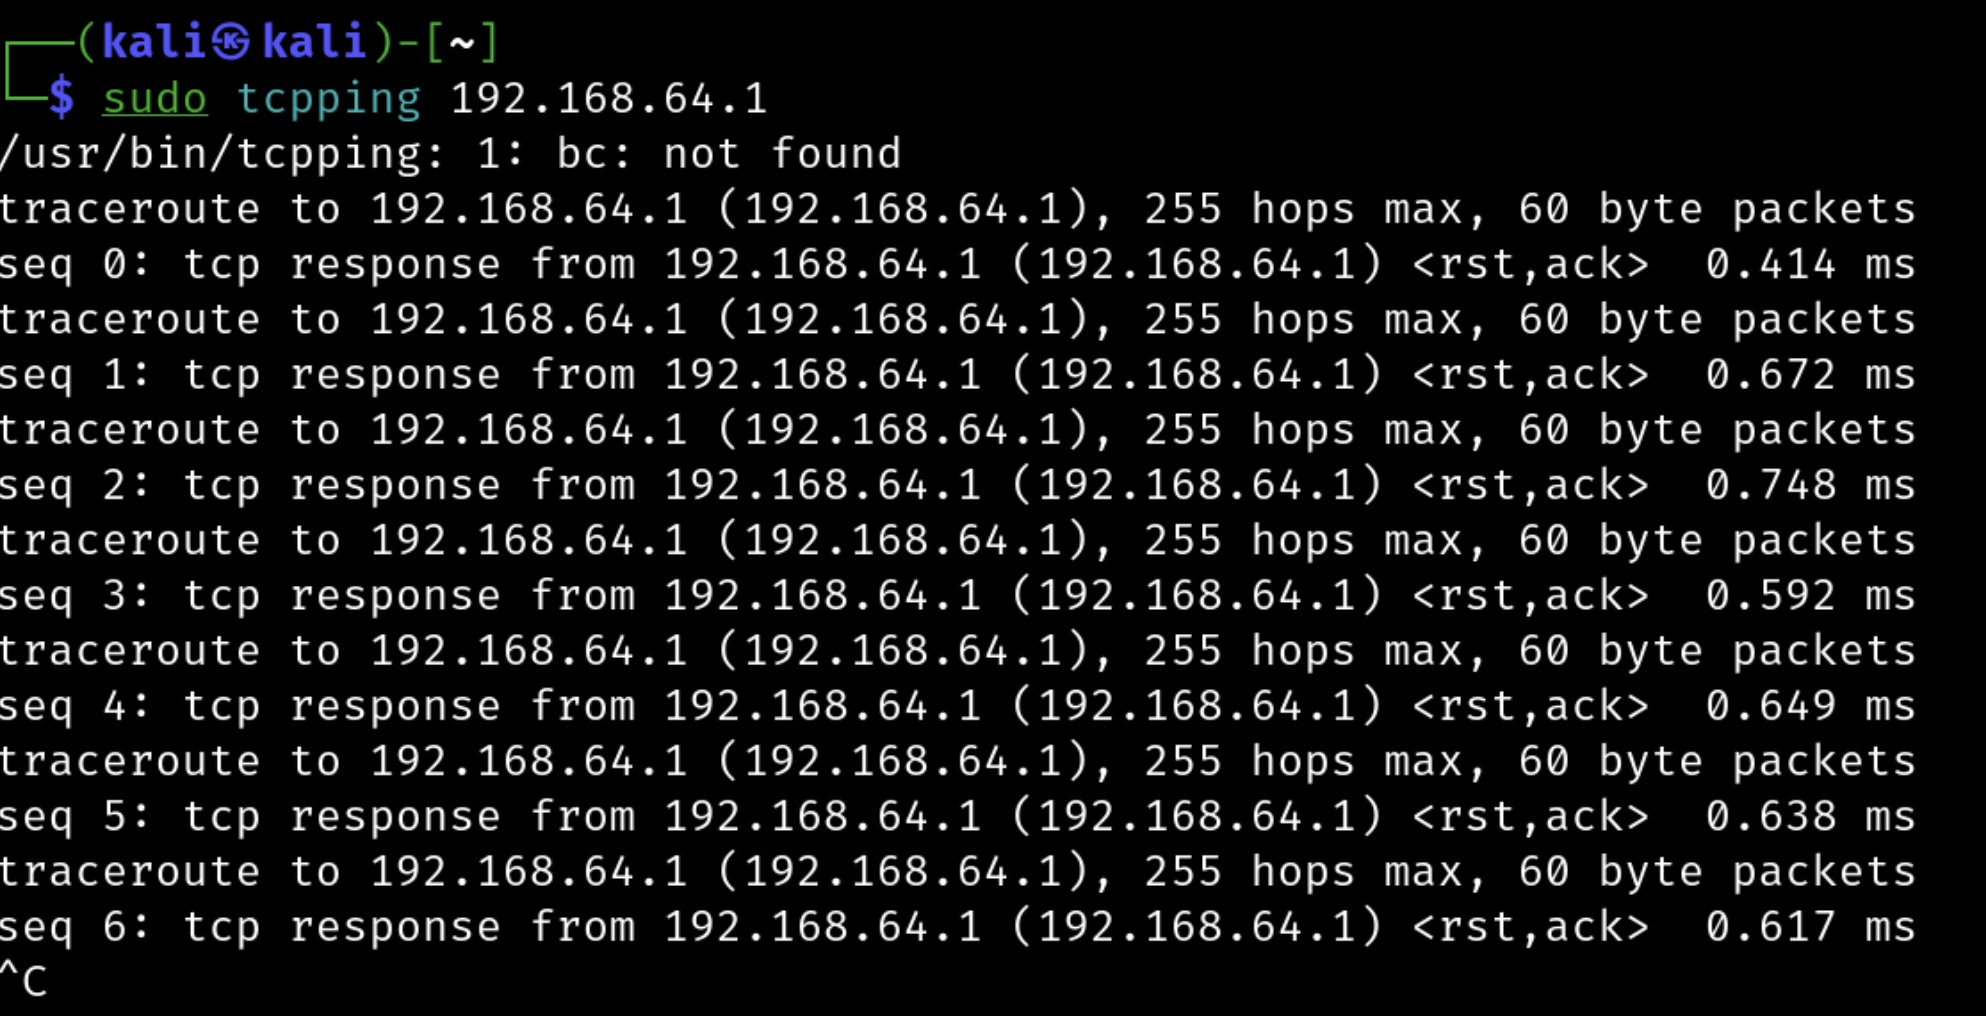
\includegraphics[width=.7\linewidth]{Practica 3y4/images/Screenshot 2024-11-07 at 20.18.44.png}
        \caption{Uso con un dispositivo en local}
        \label{fig:enter-label}
    \end{figure}
    \item \textit{¿Qué información útil le proporcionaría tcpping desde el punto de vista de la seguridad?}
    \newline
    \newline
    Desde una perspectiva de la seguridad, este comando puede proporcionarnos información valiosa como la detección de servicios activos, verificación de configuración de algún firewall, la latencia y el rendimiento de la red, entre otros.
\end{itemize}
%%%%%%%%%%%%%%%%%%%%%%%%%%%%%%%%%%%%%%%%%%%%%%%%%%%%%%%%
\section{Ejercicio 2}
\textit{Accedemos a la siguiente máquina de TryHackme~\cite{TryHackmeNmapRoom}}
\begin{itemize}
    \item \textit{Acceda a la documentación de Nmap~\cite{Nmap}. Describa la sintaxis completa con las opciones del comando nmap.}
    \newline
    \newline
\verb|nmap [<Scan Type>...] [<Options>] {<target specification>}|
    \item \textit{Realice un escaneo en modo half-scan de la máquina objetivo.}
    \newline
    \newline
    Un escaneo denominado \textit{half-scan} es aquel donde no se completa el saludo de 3 vías, por tanto, para poder realizarlo haremos uso de la opción \texttt{-sS}, además con \texttt{-p-} especificamos todo el rango de puertos abiertos.
    Todo esto lo podemos ver en \hyperlink{Nmap Half-Scan}{https://nmap.org/book/synscan.html}

    \begin{figure}[h]
        \centering
        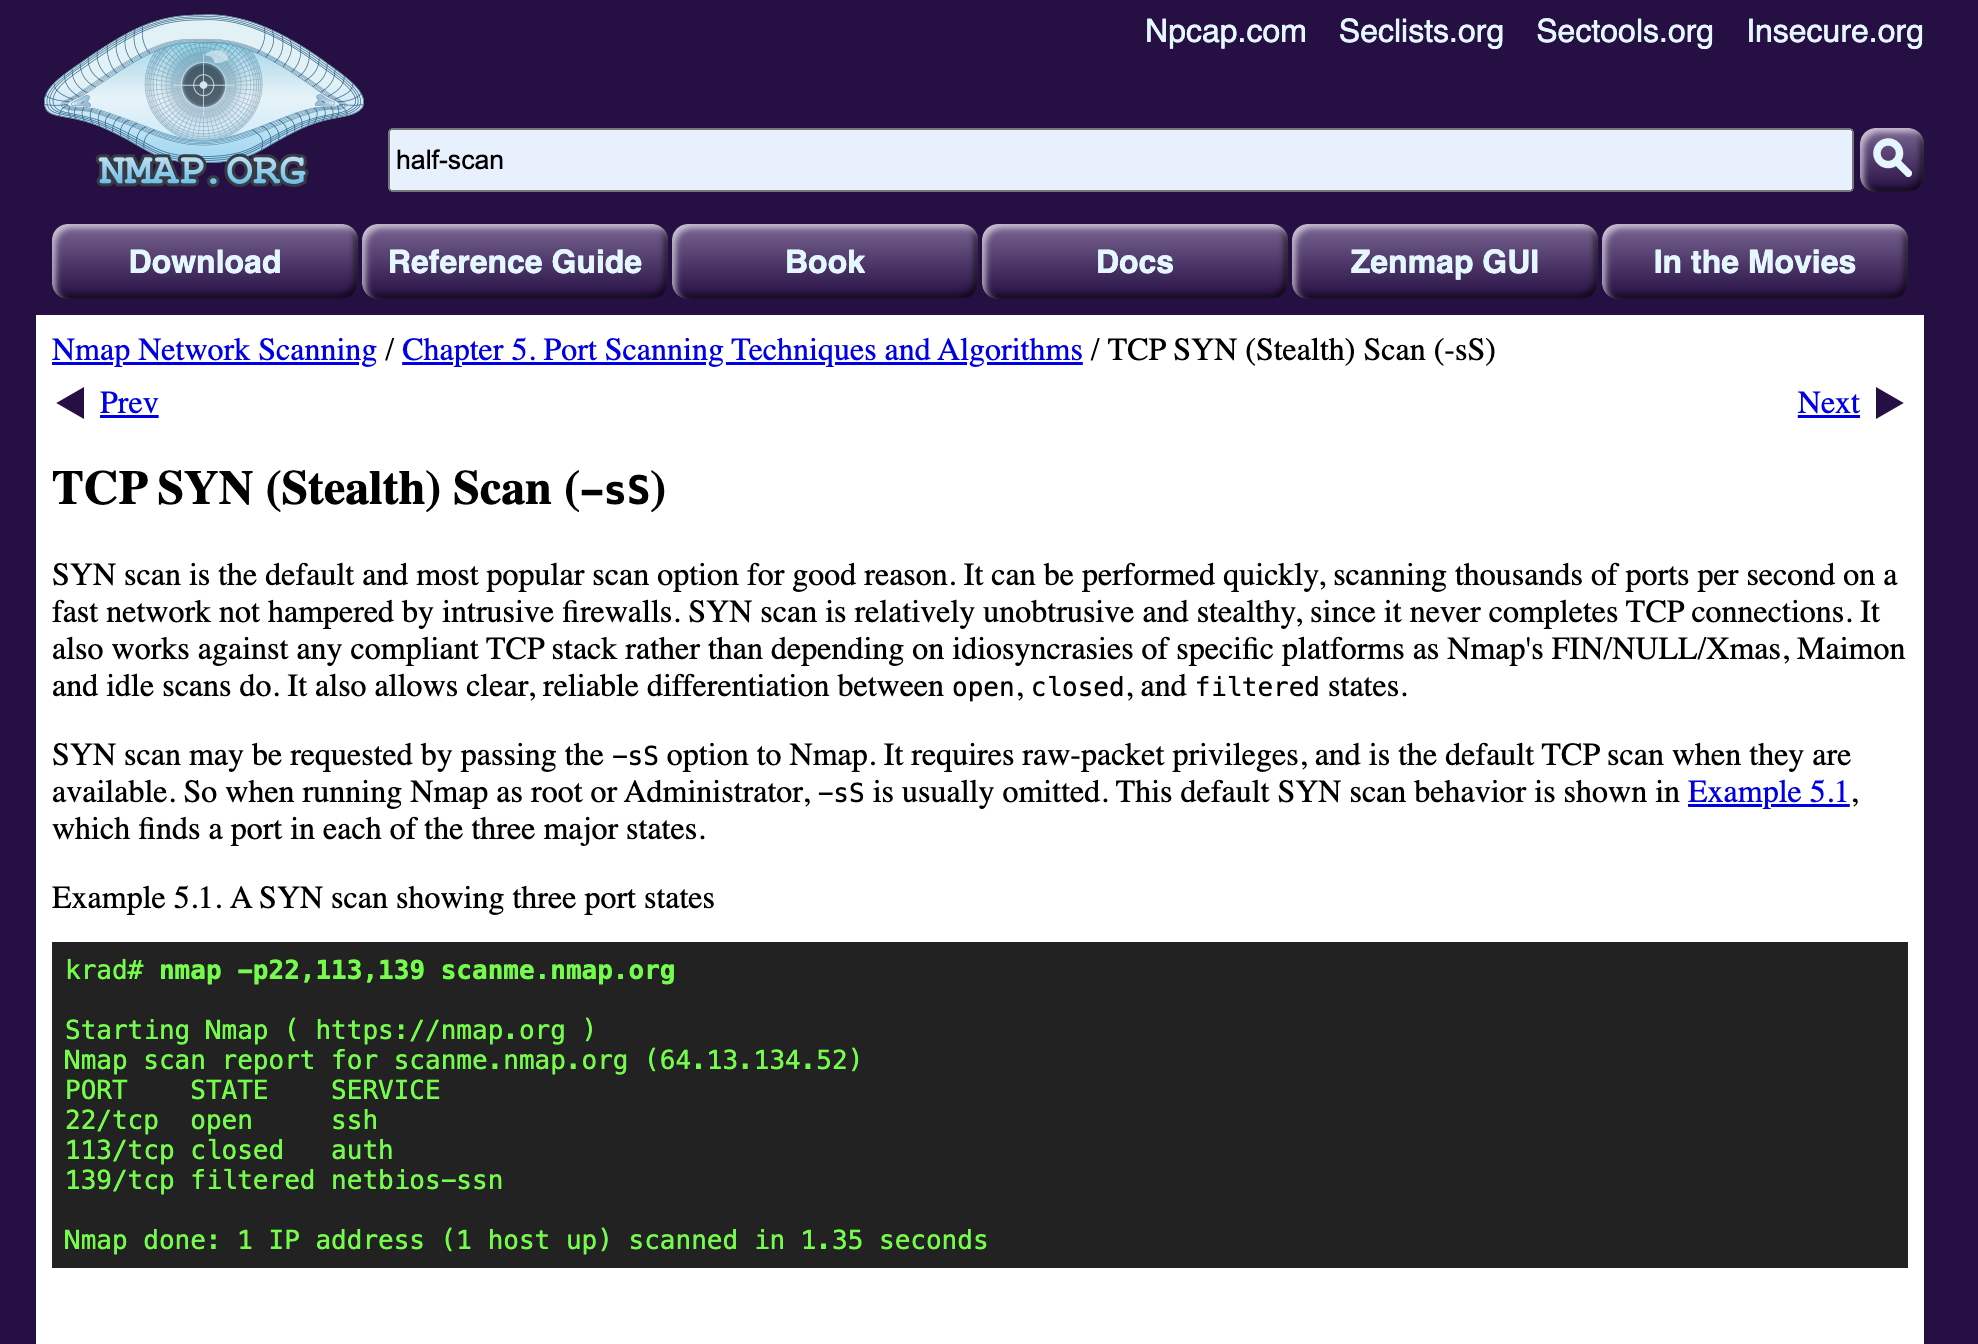
\includegraphics[width=.7\linewidth]{Practica 3y4/images/Screenshot 2024-11-07 at 09.44.38.png}
        \caption{Búsqueda del tipo escaneo}
        \label{fig:enter-label}
    \end{figure}
    
    Ahora, lo ponemos en práctica frente a la IP de la máquina víctima dada por la plataforma:
    \begin{figure}[h]
        \centering
        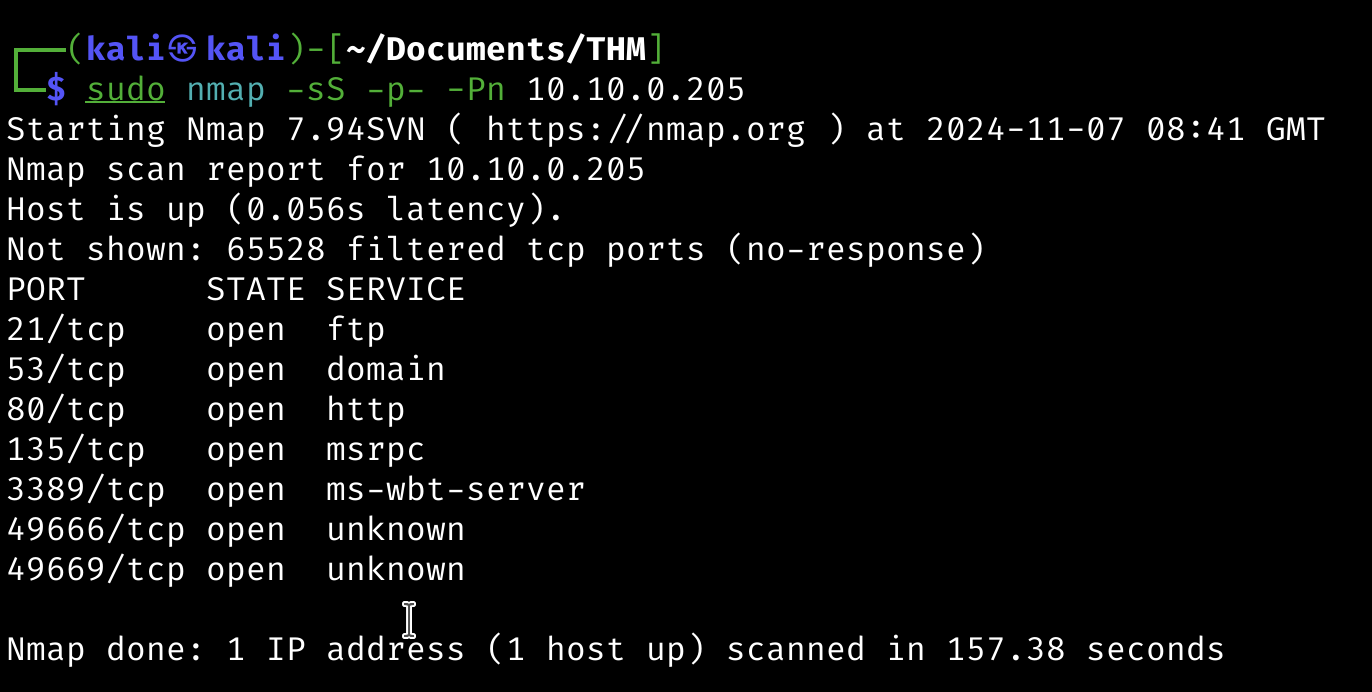
\includegraphics[width=.6\linewidth]{Practica 3y4/images/Screenshot 2024-11-07 at 09.46.03.png}
        \caption{Resutlado del half-scan de Nmap}
        \label{fig:enter-label}
    \end{figure}
    \newpage
    \item \textit{Realice un escaneo tipo connect que permita detectar el sistema operativo de la
máquina objetivo.}
    \newline
    \newline
    Ahora, volvemos a buscar en la misma web el nuevo escaneo. En este caso el parámetro será \texttt{-sT}, donde realiza una conexión \textit{TCP} con el servidor.
    \newline
    A diferencia de la opción anterior, es decir \texttt{-sS}, el escaneo si realiza el saludo de 3 vías del protocolo TCP.
    
    \begin{figure}[h]
        \centering
        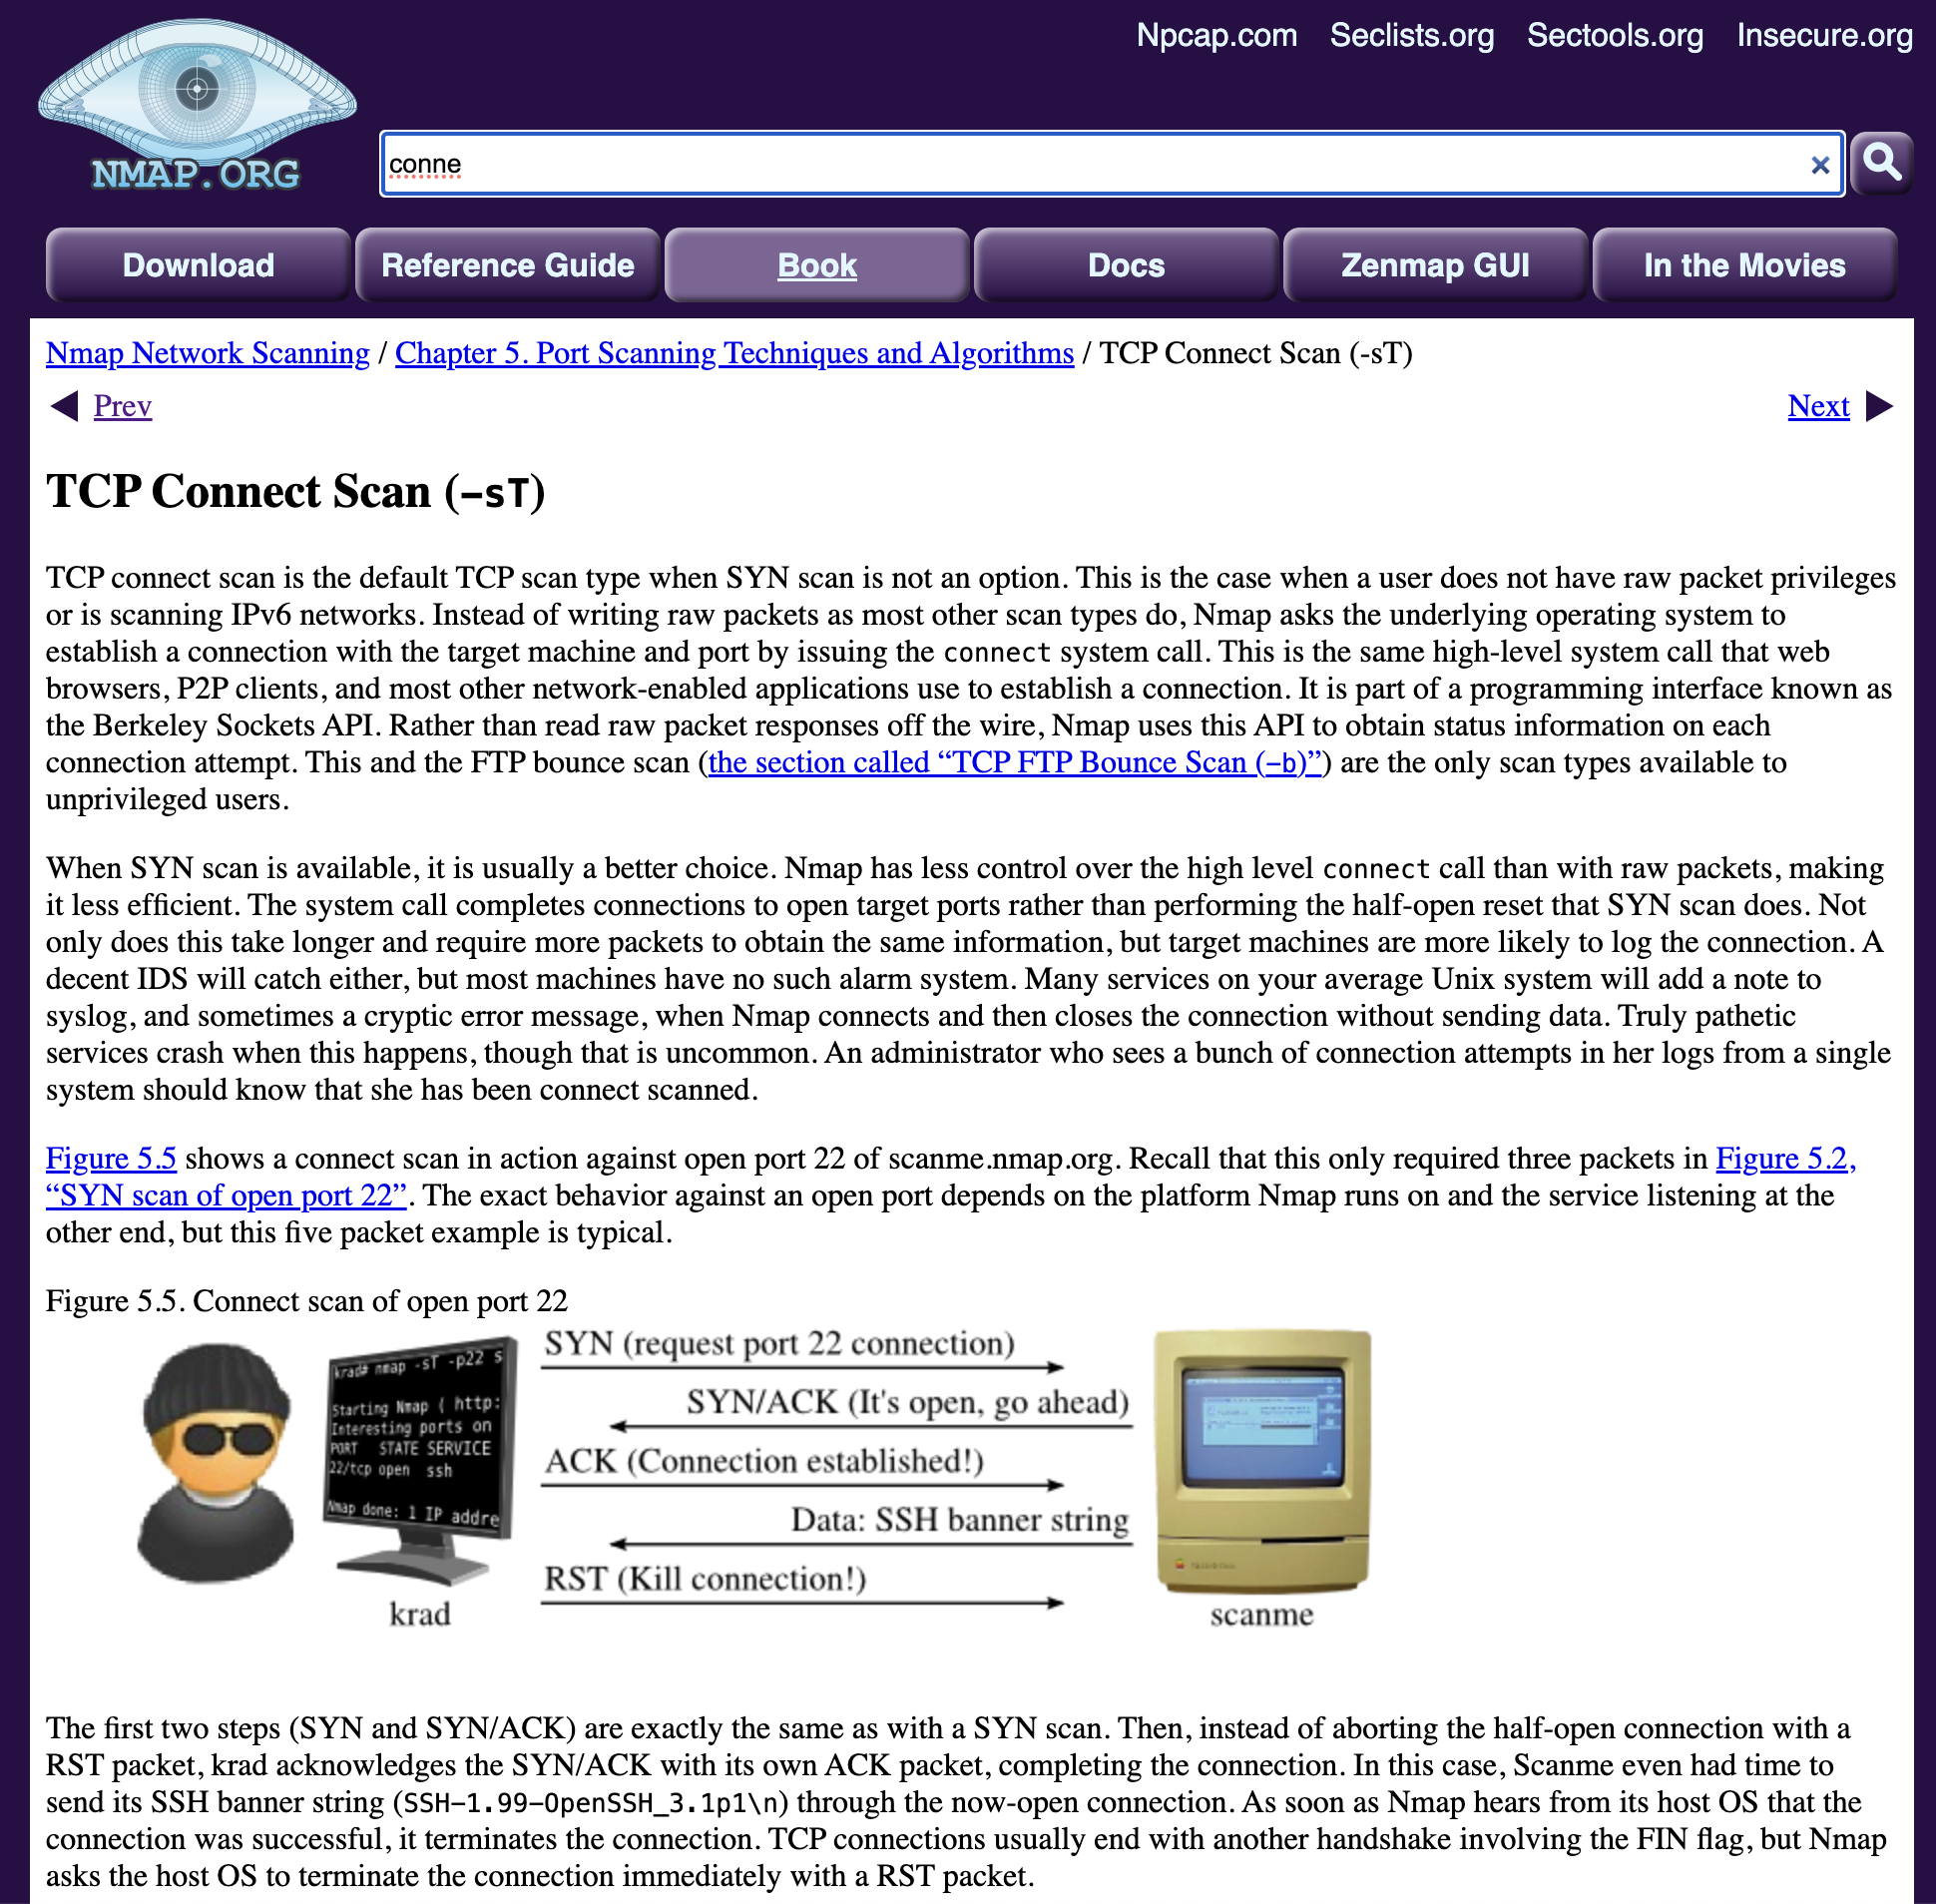
\includegraphics[width=.5\linewidth]{Practica 3y4/images/Screenshot 2024-11-07 at 09.48.36.png}
        \caption{Búsqueda del escaneo}
        \label{fig:enter-label}
    \end{figure}

    Lo ponemos en práctica:
    \begin{figure}[h]
        \centering
        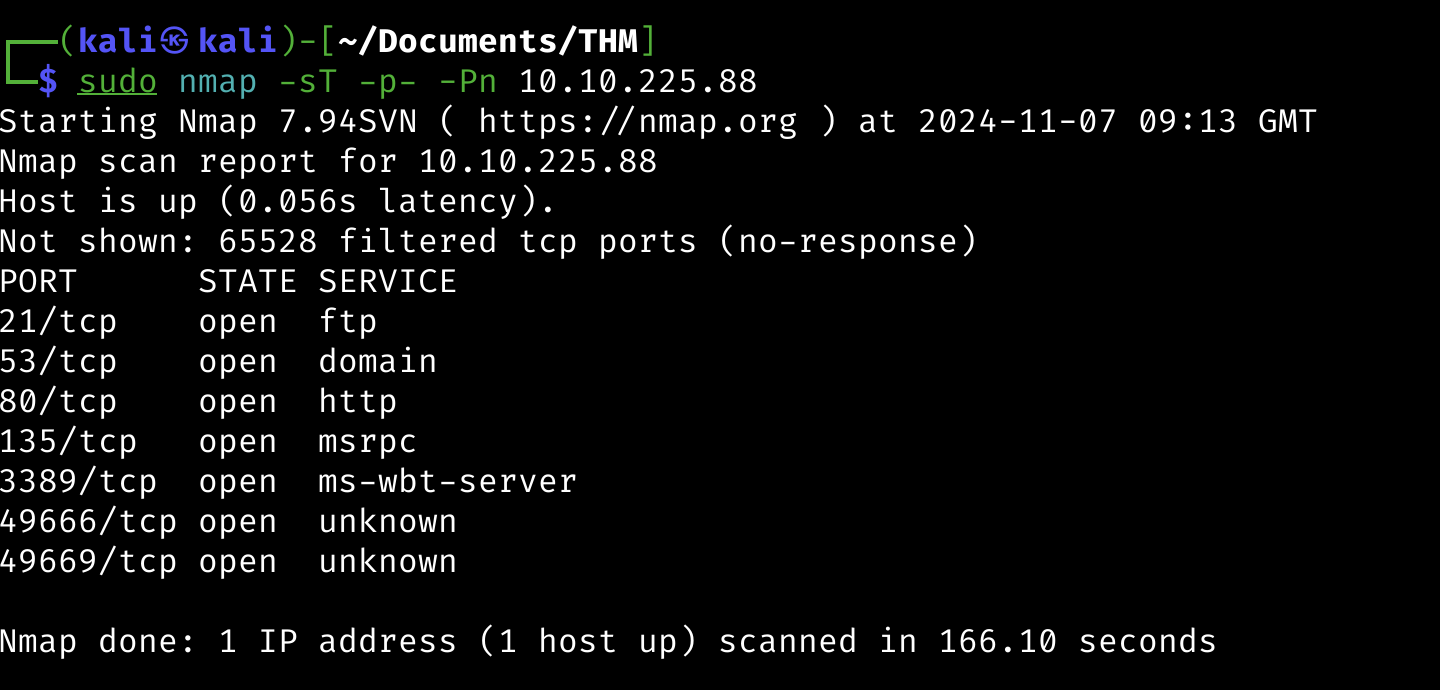
\includegraphics[width=.7\linewidth]{Practica 3y4/images/Screenshot 2024-11-07 at 10.18.23.png}
        \caption{Resultado del escaneo connect.}
        \label{fig:enter-label}
    \end{figure}
    \newpage
    \item \textit{Realice un escaneo en modo half-scan que permita detectar el sistema operativo, la versión de los servicios y la obtención de banners de la máquina objetivo.}
    \newline
    \newline
    Para poder realizar este tipo de ataque, vamos a hacer uso de las opciones \texttt{-sS} para un ataque de tipo \textit{half-scan}, el parámetro \texttt{--script} donde le especificamos que queremos los \textit{banners} y la opción \texttt{-sV} para obtener la versión (esto, al igual que los escaneos anteriores lo busqué en la web de Nmap):
    \begin{figure}[h]
        \centering
        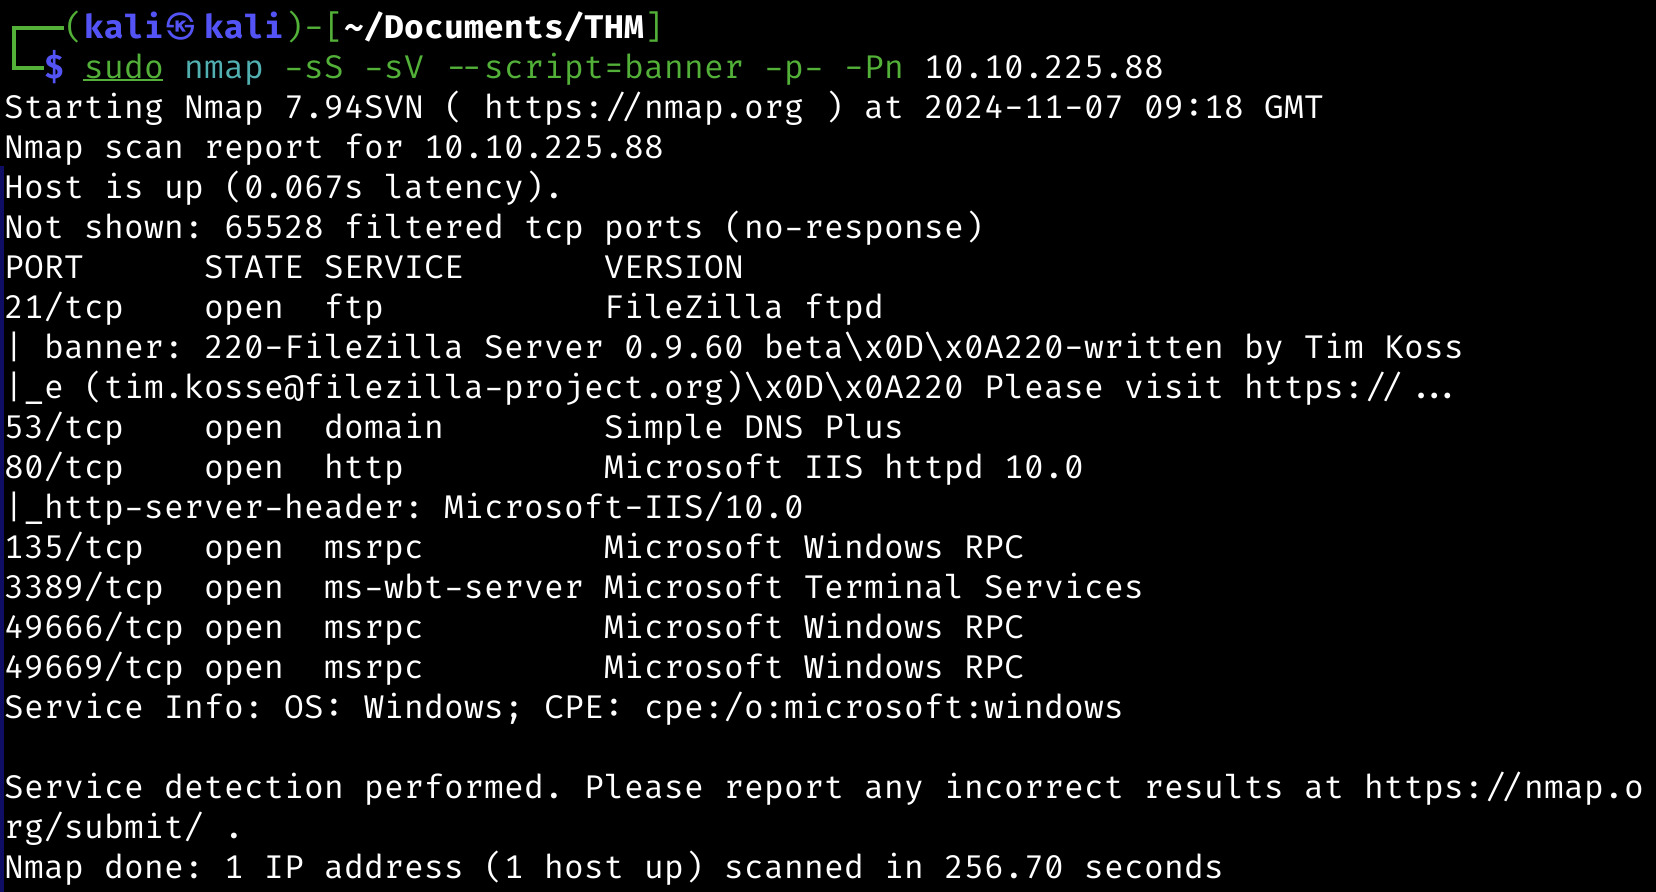
\includegraphics[width=.7\linewidth]{Practica 3y4/images/Screenshot 2024-11-07 at 10.23.11.png}
        \caption{Escaneo que nos devuelve las versiones de los protocolos}
        \label{fig:enter-label}
    \end{figure}
\end{itemize}
\newpage
%%%%%%%%%%%%%%%%%%%%%%%%%%%%%%%%%%%%%%%%%%%%%%%%%%%%%%%%
\section{Ejercicio 3}
\textit{Describa y explique los resultados obtenidos tras ejecutar el comando nmap en Kali
Linux junto con las opciones necesarias para realizar:}
\begin{itemize}
    \item\textit{Un escaneo en modo half-scan del servidor scanme.nmap.org.}\\
    \begin{figure}[h]
        \centering
        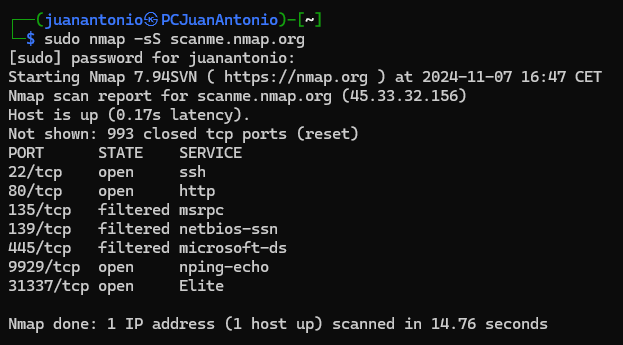
\includegraphics[width=0.7\linewidth]{Practica 3y4/images/Captura de pantalla 2024-11-07 164902.png}
        \caption{Escaneo half-open}
        \label{fig:enter-label}
    \end{figure}
    \item\textit{Un escaneo tipo connect que permita detectar el sistema operativo del servidor scanme.nmap.org.}\\
    Obtenemos los puertos abiertos y su servicio.
    \begin{figure}[h]
        \centering
        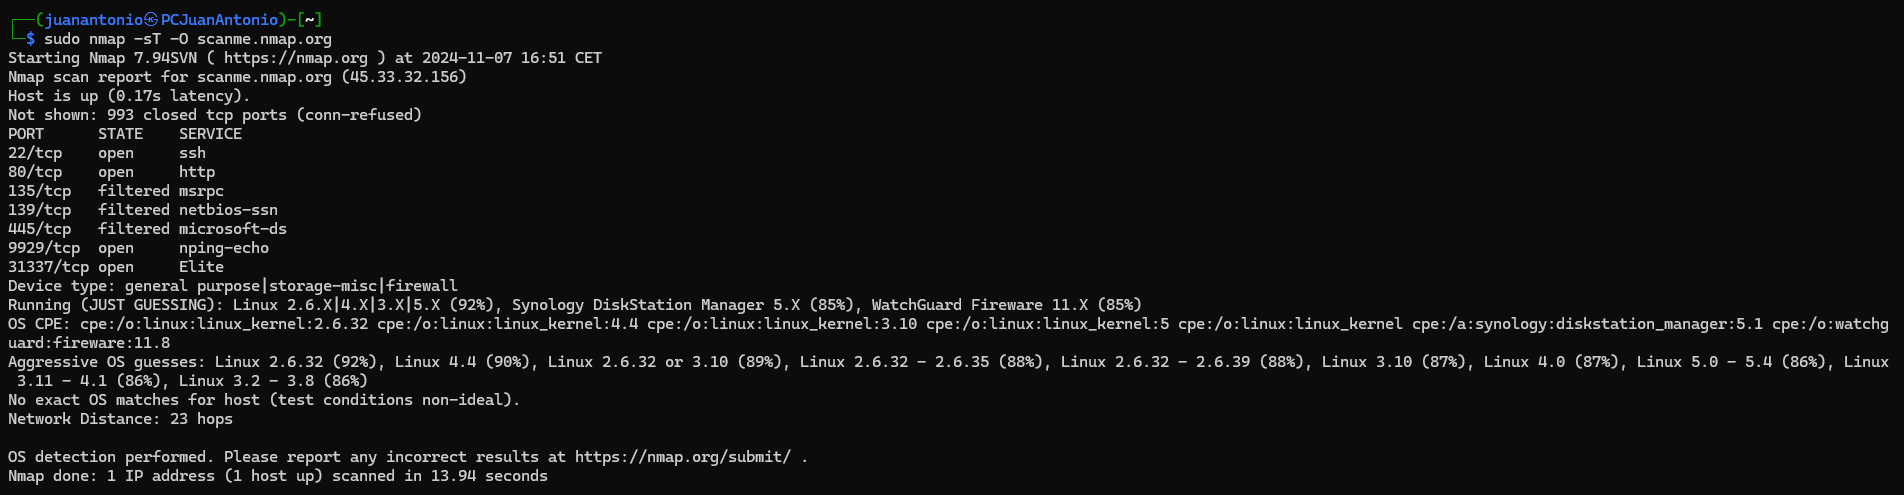
\includegraphics[width=\linewidth]{Practica 3y4/images/Captura de pantalla 2024-11-07 165209.png}
        \caption{Escaneo Connect() con SO}
        \label{fig:enter-label}
    \end{figure}
    \\
    En este caso no se puede obtener el sistema operativo con certeza pero nos da una aproximación. De igual manera que en caso anterior, obtenemos los puertos abiertos y sus servicios.
    \newpage
    \item\textit{Un escaneo en modo half-scan que permita detectar el sistema operativo, la versión de los servicios y la obtención de banners del servidor scanme.nmap.org.}\\
    \begin{figure}[h]
        \centering
        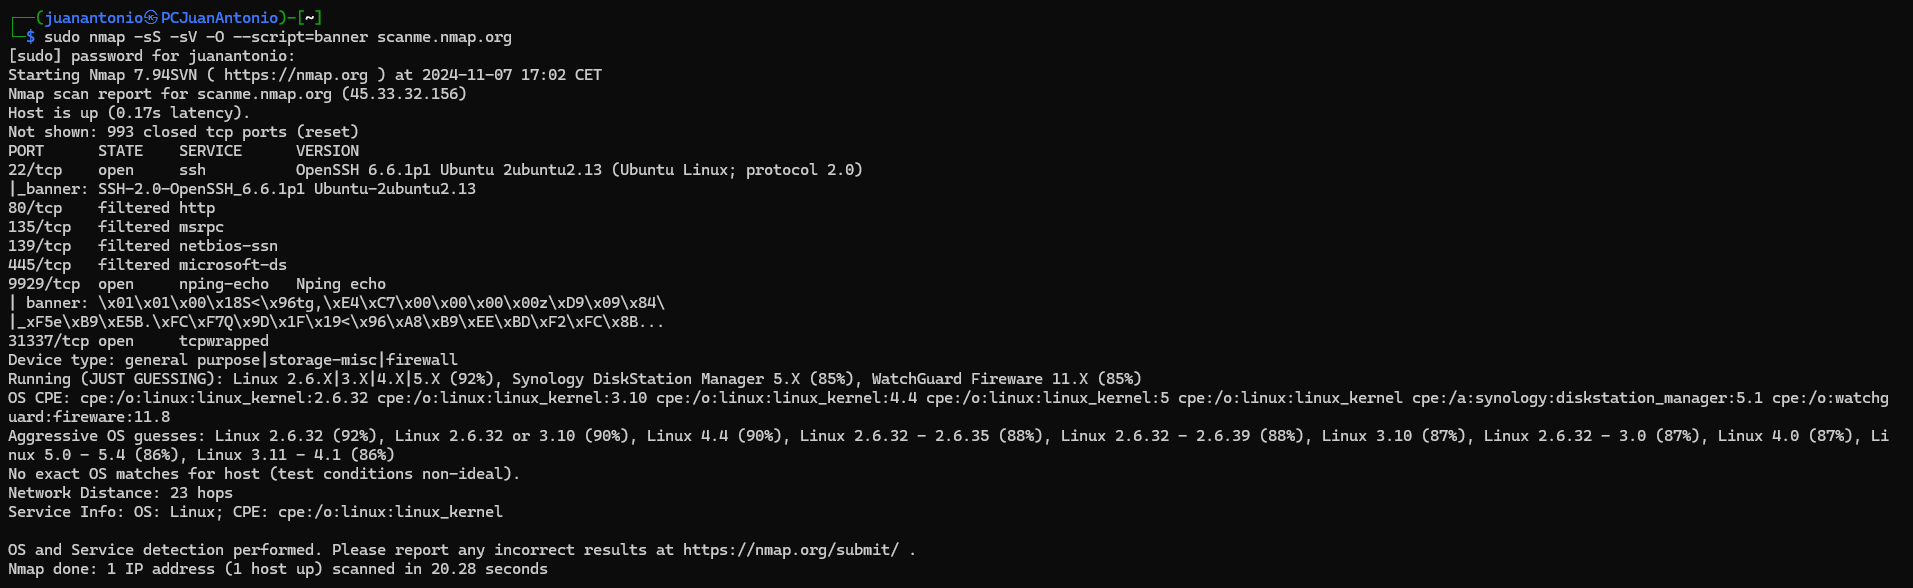
\includegraphics[width=\linewidth]{Practica 3y4/images/Captura de pantalla 2024-11-07 170333.png}
        \caption{Escaneo half-open con SO, versión de servicios y banners}
        \label{fig:enter-label}
    \end{figure}\\
    obtenemos lo mismo que en la primera consulta, pero ahora tenemos la versión de algunos puertos y de igual forma, se muestran, algunos banners.
    \end{itemize}
%%%%%%%%%%%%%%%%%%%%%%%%%%%%%%%%%%%%%%%%%%%%%%%%%%%%%%%%
\newpage
\section{Ejercicio 4}
\textit{Una vez instalada la herramienta Furious en Kali Linux, realice un escáner de tipo connect a la web oficial de la universidad:\\
\textbf{uca.es}\\
    \begin{figure}[h]
        \centering
        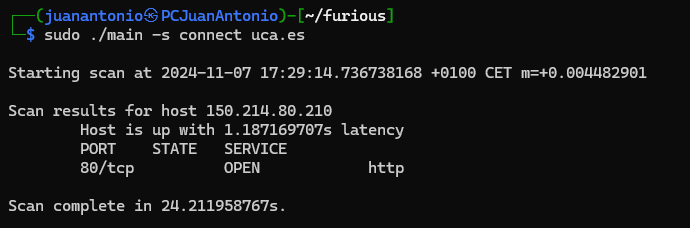
\includegraphics[width=\linewidth]{Practica 3y4/images/Captura de pantalla 2024-11-07 172956.png}
        \caption{Uso de Furious para escaneo de uca.es}
        \label{fig:enter-label}
    \end{figure}\\
Una vez realizado, responda a las siguientes preguntas:\\}
\begin{itemize}
    \item \textit{¿Cuál es la dirección del host?}\\
    La dirección del host es 150.214.80.210
    \item \textit{¿Tiene algún puerto abierto? En caso afirmativo, ¿cuál?}\\
    Sí, tiene abierto el puerto 80 ligado al servicio http
    \item \textit{¿Qué comando ha utilizado para realizar un escaneo de este tipo?}\\
    Hemos utilizado el comando \textbf{sudo ./main -s connect uca.es}
\end{itemize}
%%%%%%%%%%%%%%%%%%%%%%%%%%%%%%%%%%%%%%%%%%%%%%%%%%%%%%%%


\bibliography{bibliografia}
\bibliographystyle{plain}
\end{document}